\documentclass{article}

\usepackage[margin=1.25in]{geometry}
\usepackage[usenames,dvipsnames]{color}
\usepackage[colorlinks,
            linkcolor=blue,
            citecolor=blue,
            urlcolor=magenta,
            linktocpage,
            plainpages=false]{hyperref}
\usepackage{amsmath,amssymb,amsfonts,amsthm,mathtools}
\usepackage{thmtools,xcolor-patch,hyperref,graphicx}
\usepackage[lined,ruled]{algorithm2e}
\usepackage[capitalize,nameinlink]{cleveref}
\usepackage{caption,hyperref}


\title{SENG 474 \\ Data Mining Project\\}
\author{Cole Sibbald \quad Keanelek Enns \quad Quinne Gieseke \\V00906211     \quad V00875807     \quad V00884671}
\begin{document}
	\maketitle
	\newpage

\begin{center}	\textbf{Abstract} \end{center}

Census data is filled with many different types of data that some government organizations may wish to approximately organize in order to properly understand a population's needs. In many cases it is crucial for policy makers to understand the economic situation of some group of peoples.\\

In this situation, machine learning techniques may be used to better classify a close estimate of an individual's economy. For this project we will determine the economic class of individuals based off of the 1994 data set \href{https://archive.ics.uci.edu/ml/datasets/Adult}{Adult/Census Income}.
	\tableofcontents
	\newpage

	\section{Introduction}~

The topic of this paper will focus on different ways to classify the Adult/Census Income data set. This data indicates certain attributes about a person and whether or not the person makes a yearly income of greater or less than $ 50000USD $  of income per year. This dataset measures a variety of metrics such as: Age, Gender, Occupation, Level of Education among many others.\\
	
Our methodology is to test many different methods of analysis with a few different methods of preprocessed data. Using a variety of techniques to make the data more readable. This includes working with a standardized data set, a data set using only the optimally chosen features, and lastly a PCA extracted data set used to shrink the dimensionality of the data while maintaining the distance measure between points.\\

With these slightly altered matrix values based on the same data set, we will then run a few different machine learning algorithms from Python's \emph{sklearn} library in order to determine the strengths and weaknesses of certain algorithms on varying data formats. For a record of all computations and processing performed, refer to the Project.ipynb notebook included with this report.

	\section{Data Processing}~
		Raw data is rarely in a useable format. Here we discuss our approach to retrieving, cleaning, transforming, and extracting the data in our data set.
		\subsection{Retrieval/Cleaning}~
		
		The data was retrieved from the UCI	Machine Learning Libraries under the title of \href{https://archive.ics.uci.edu/ml/datasets/Adult}{"Adult"}\\
		
		Before any data cleaning took place, the following histograms were generated in order to get an idea of the distribution of values in the data set:
		
		\begin{center}
			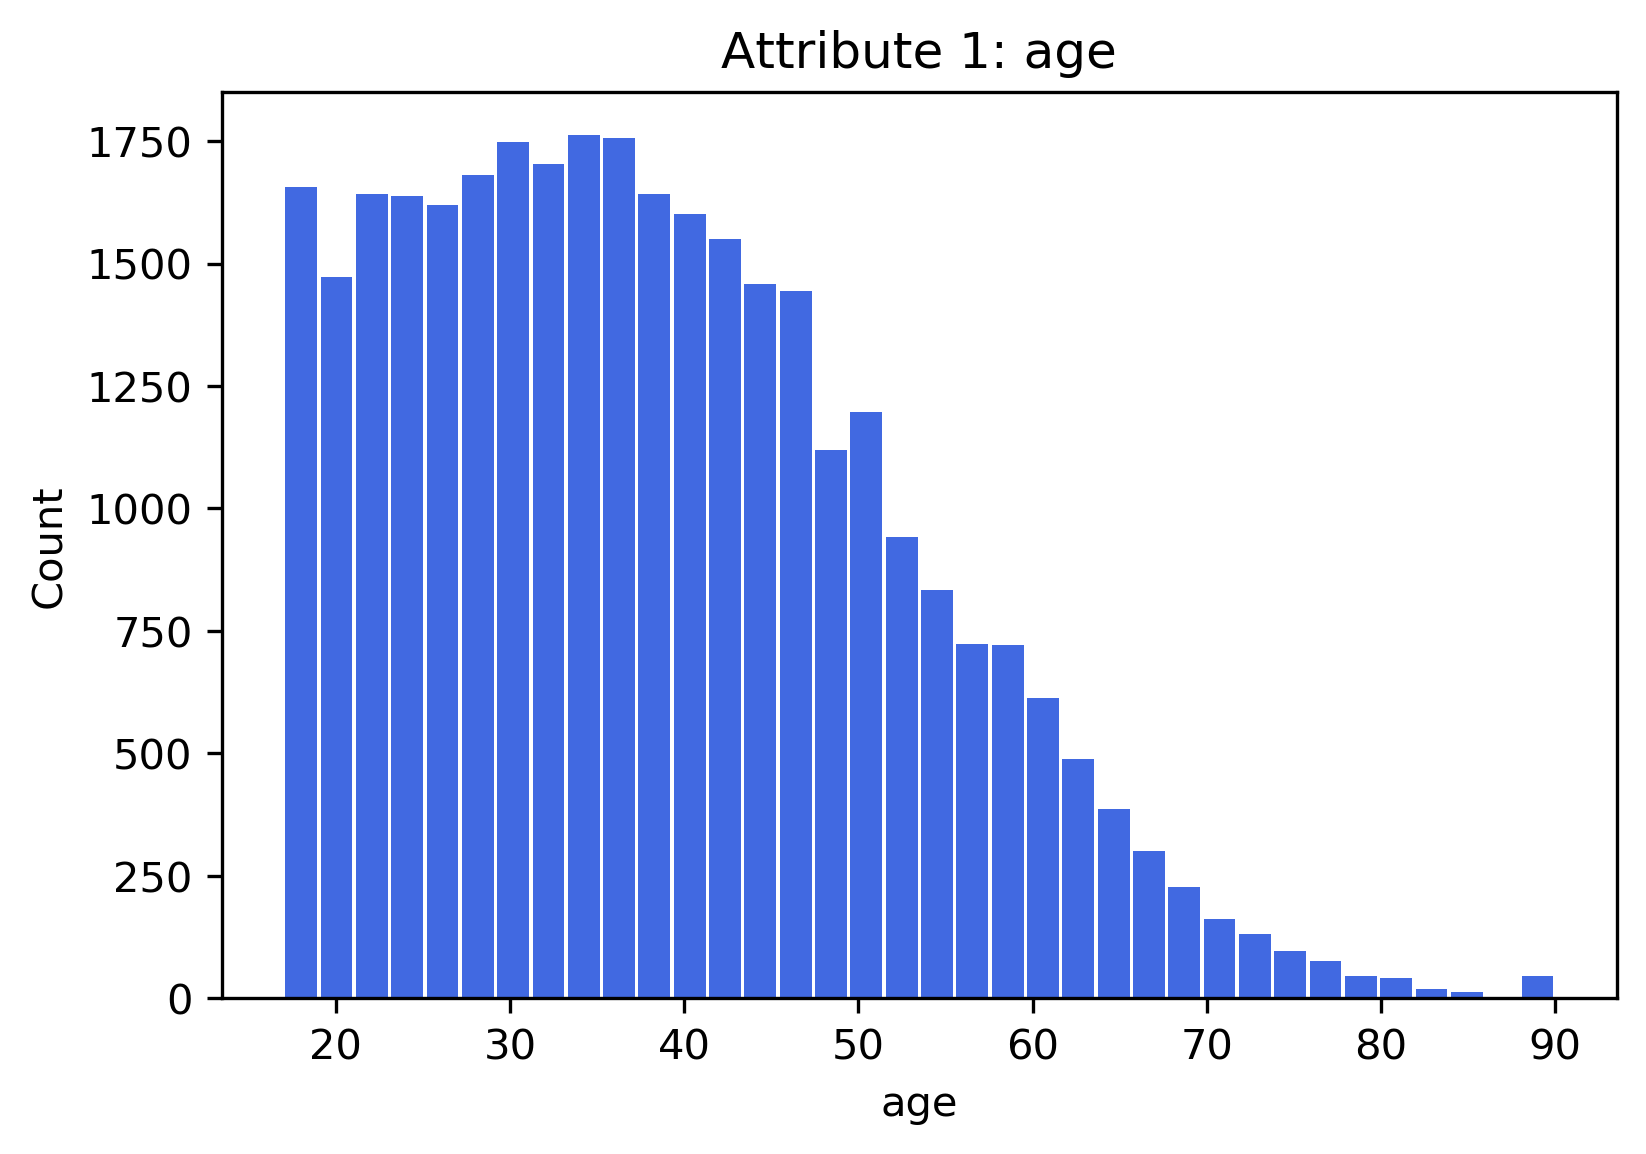
\includegraphics[width=.32\textwidth]{images/0.png}
			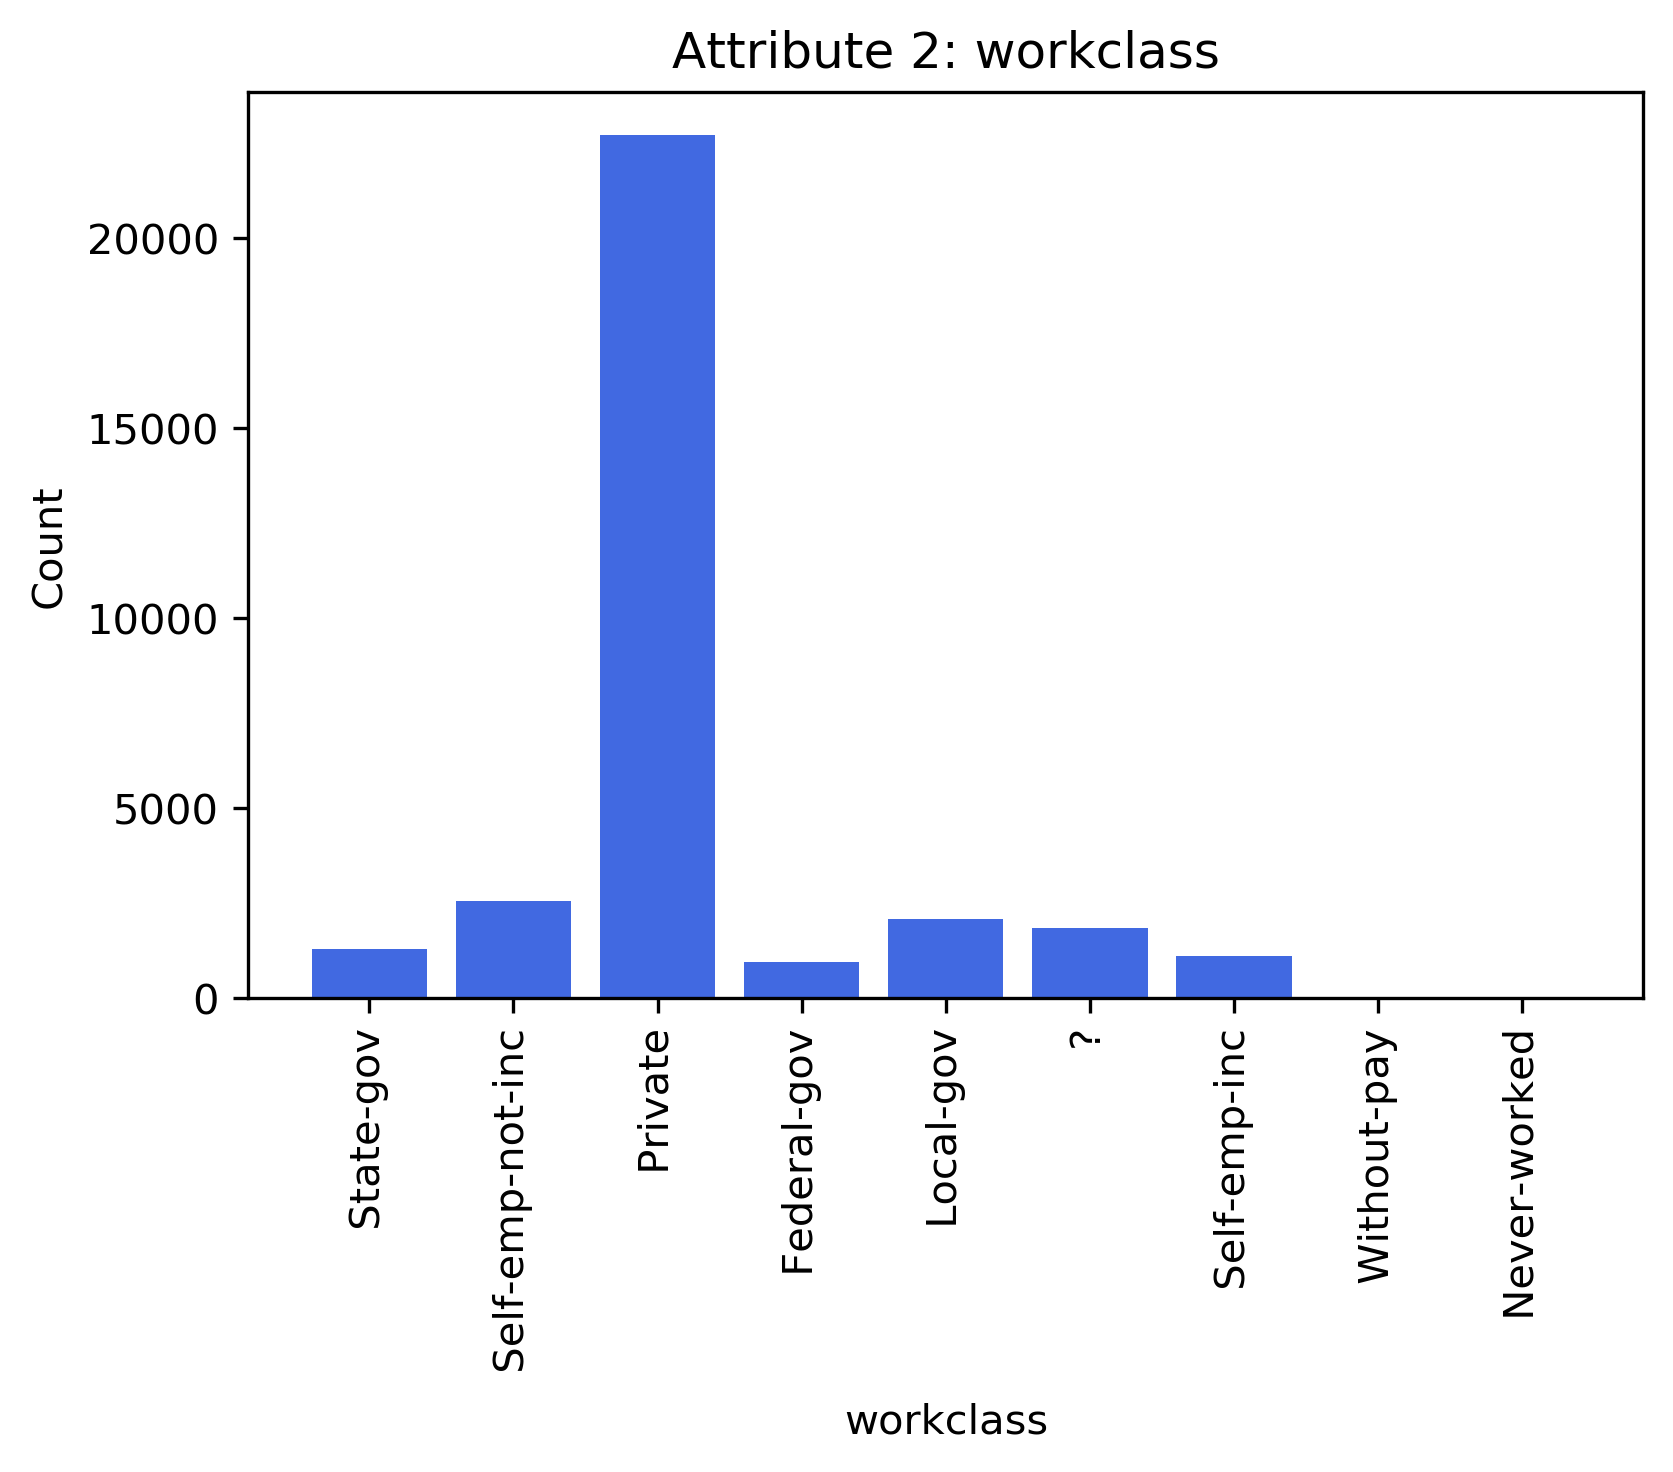
\includegraphics[width=.32\textwidth]{images/1.png}
			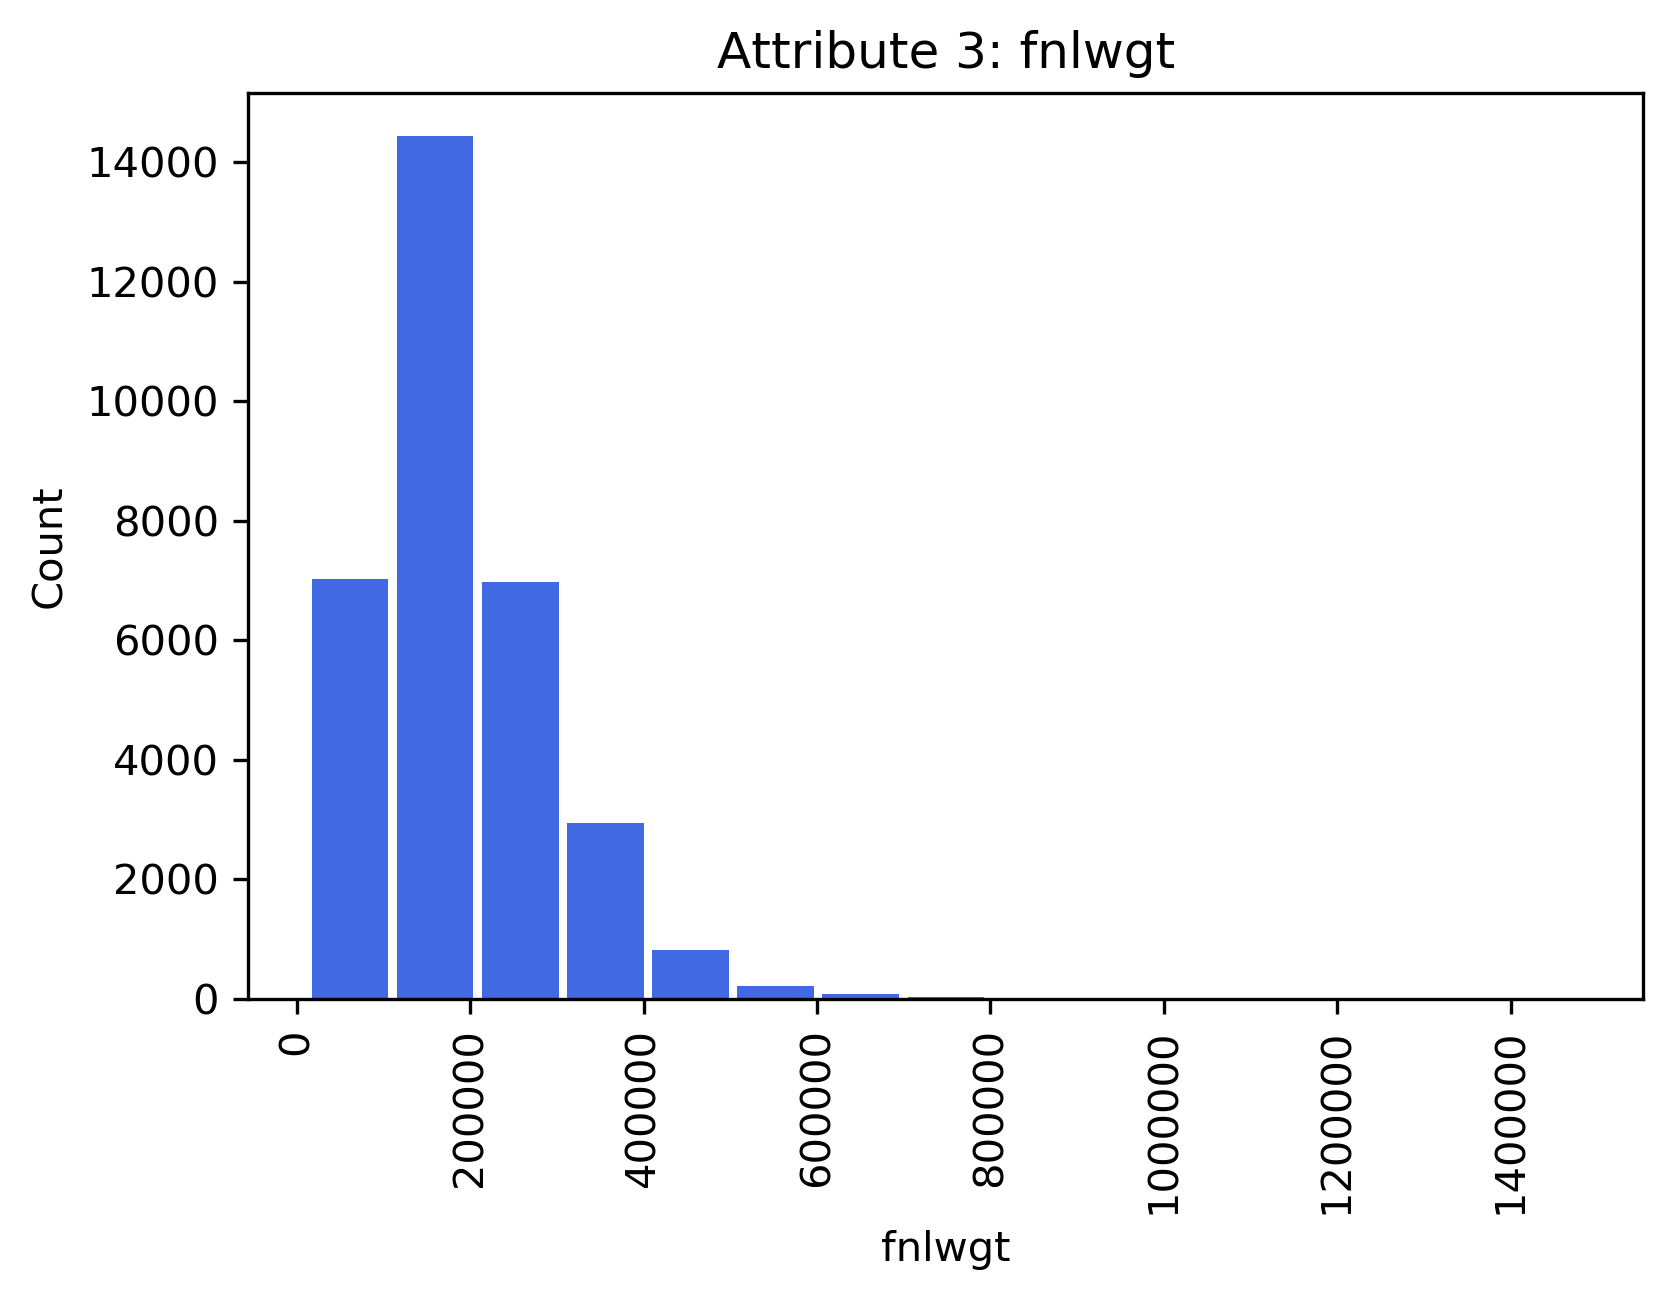
\includegraphics[width=.32\textwidth]{images/2.png}
			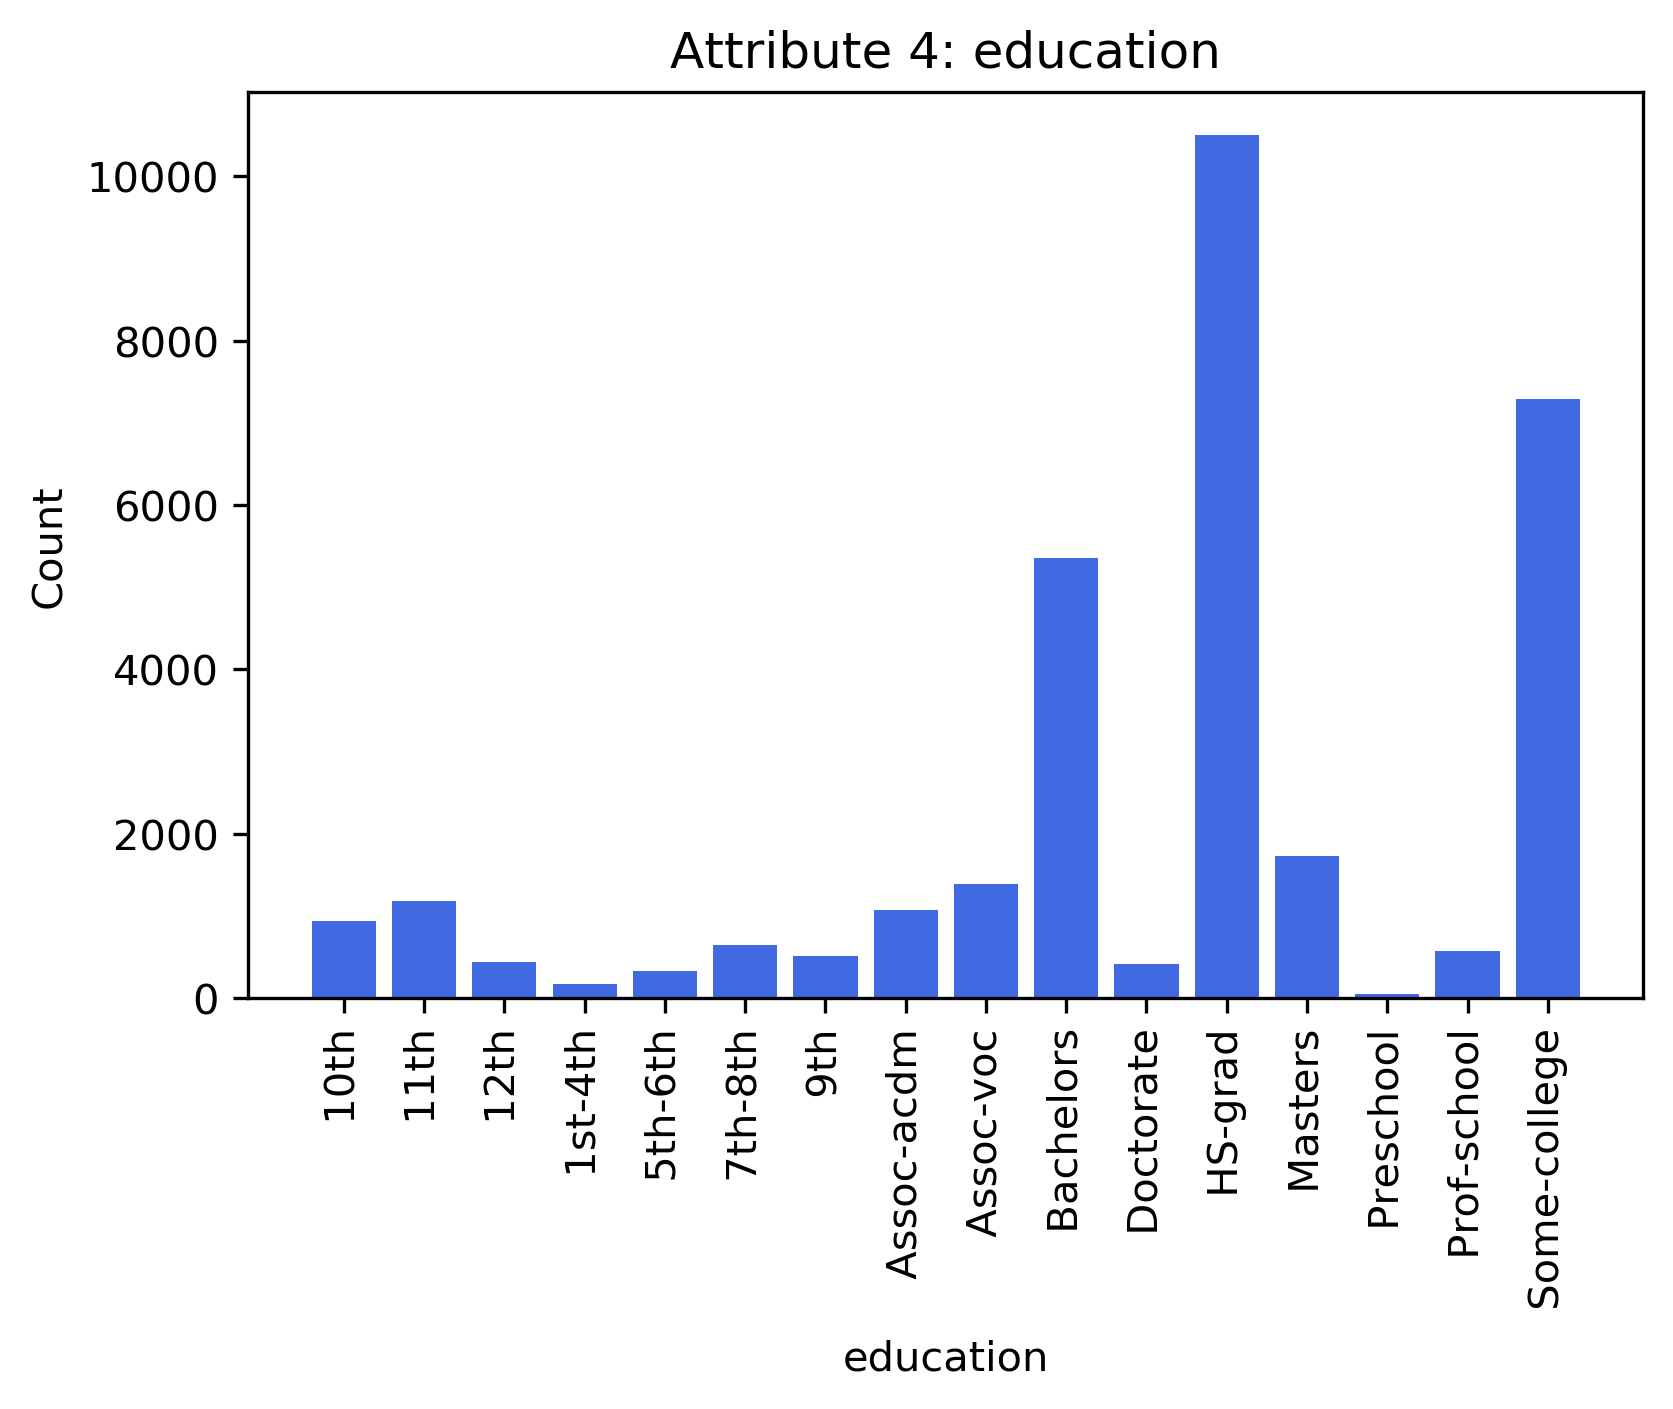
\includegraphics[width=.32\textwidth]{images/3.png}		
			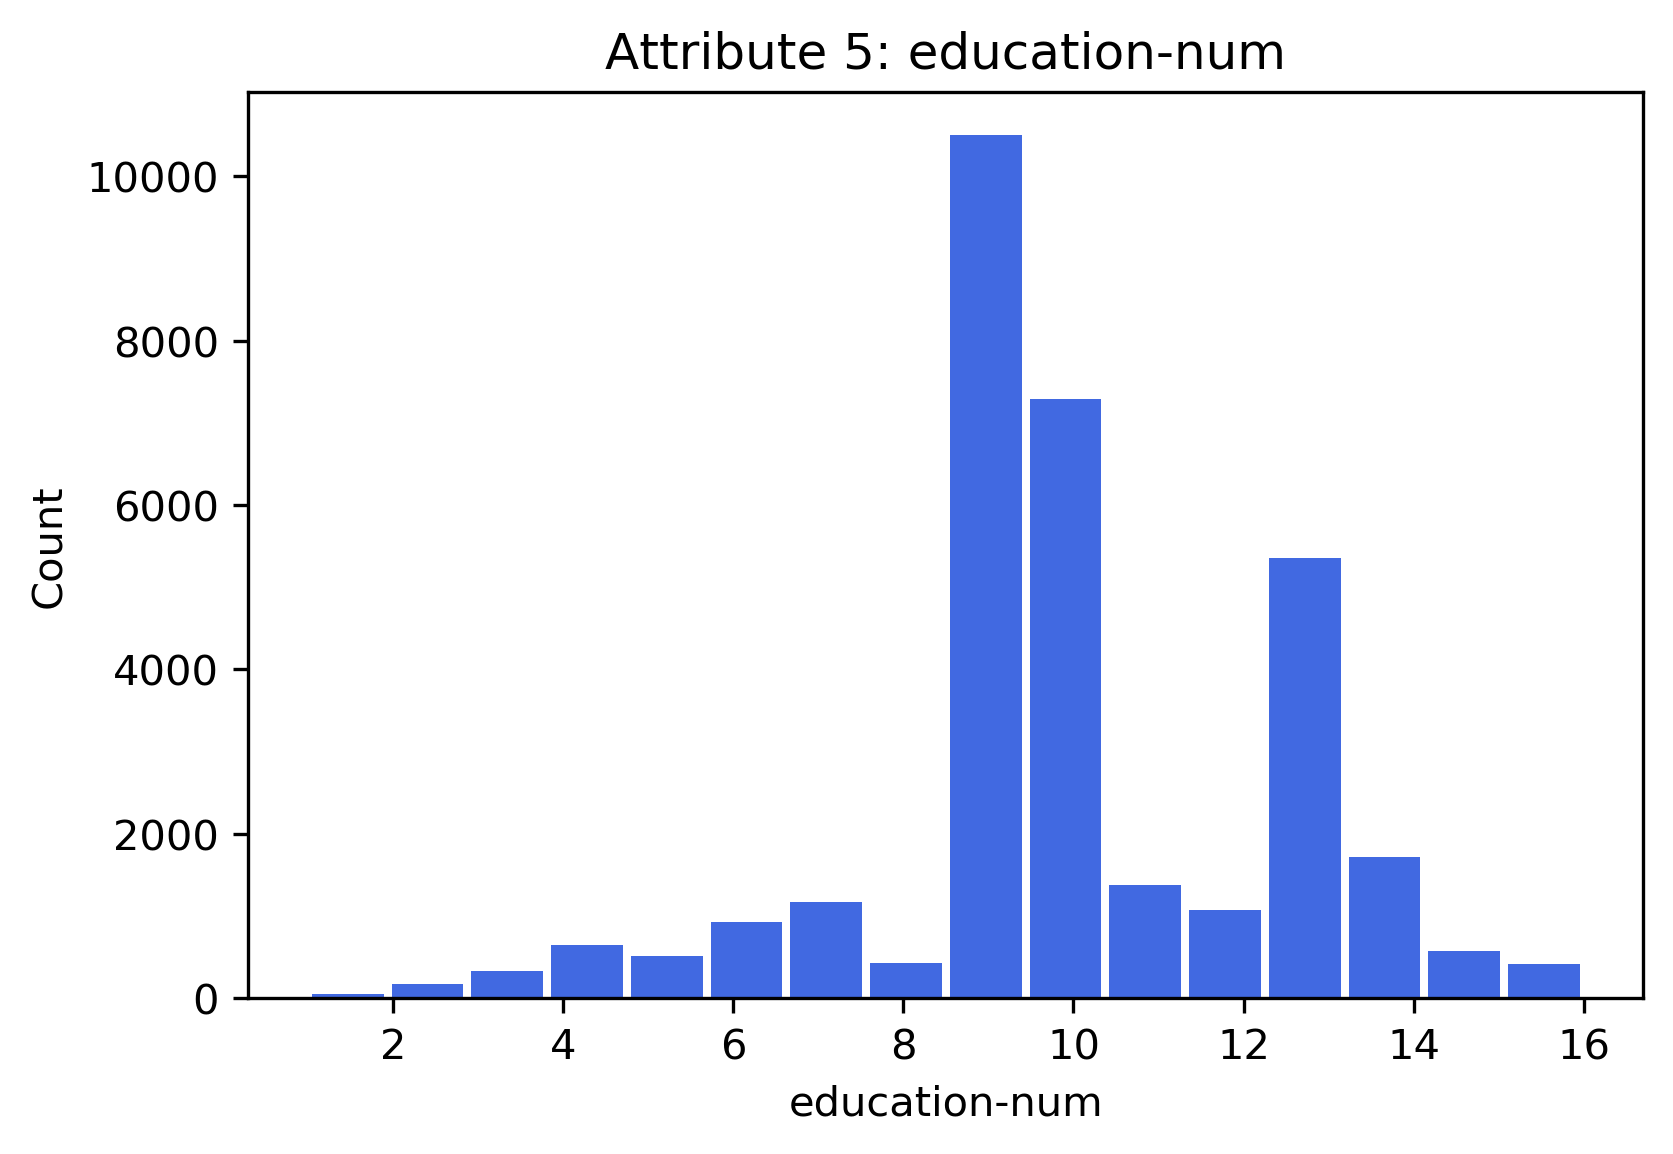
\includegraphics[width=.32\textwidth]{images/4.png}
			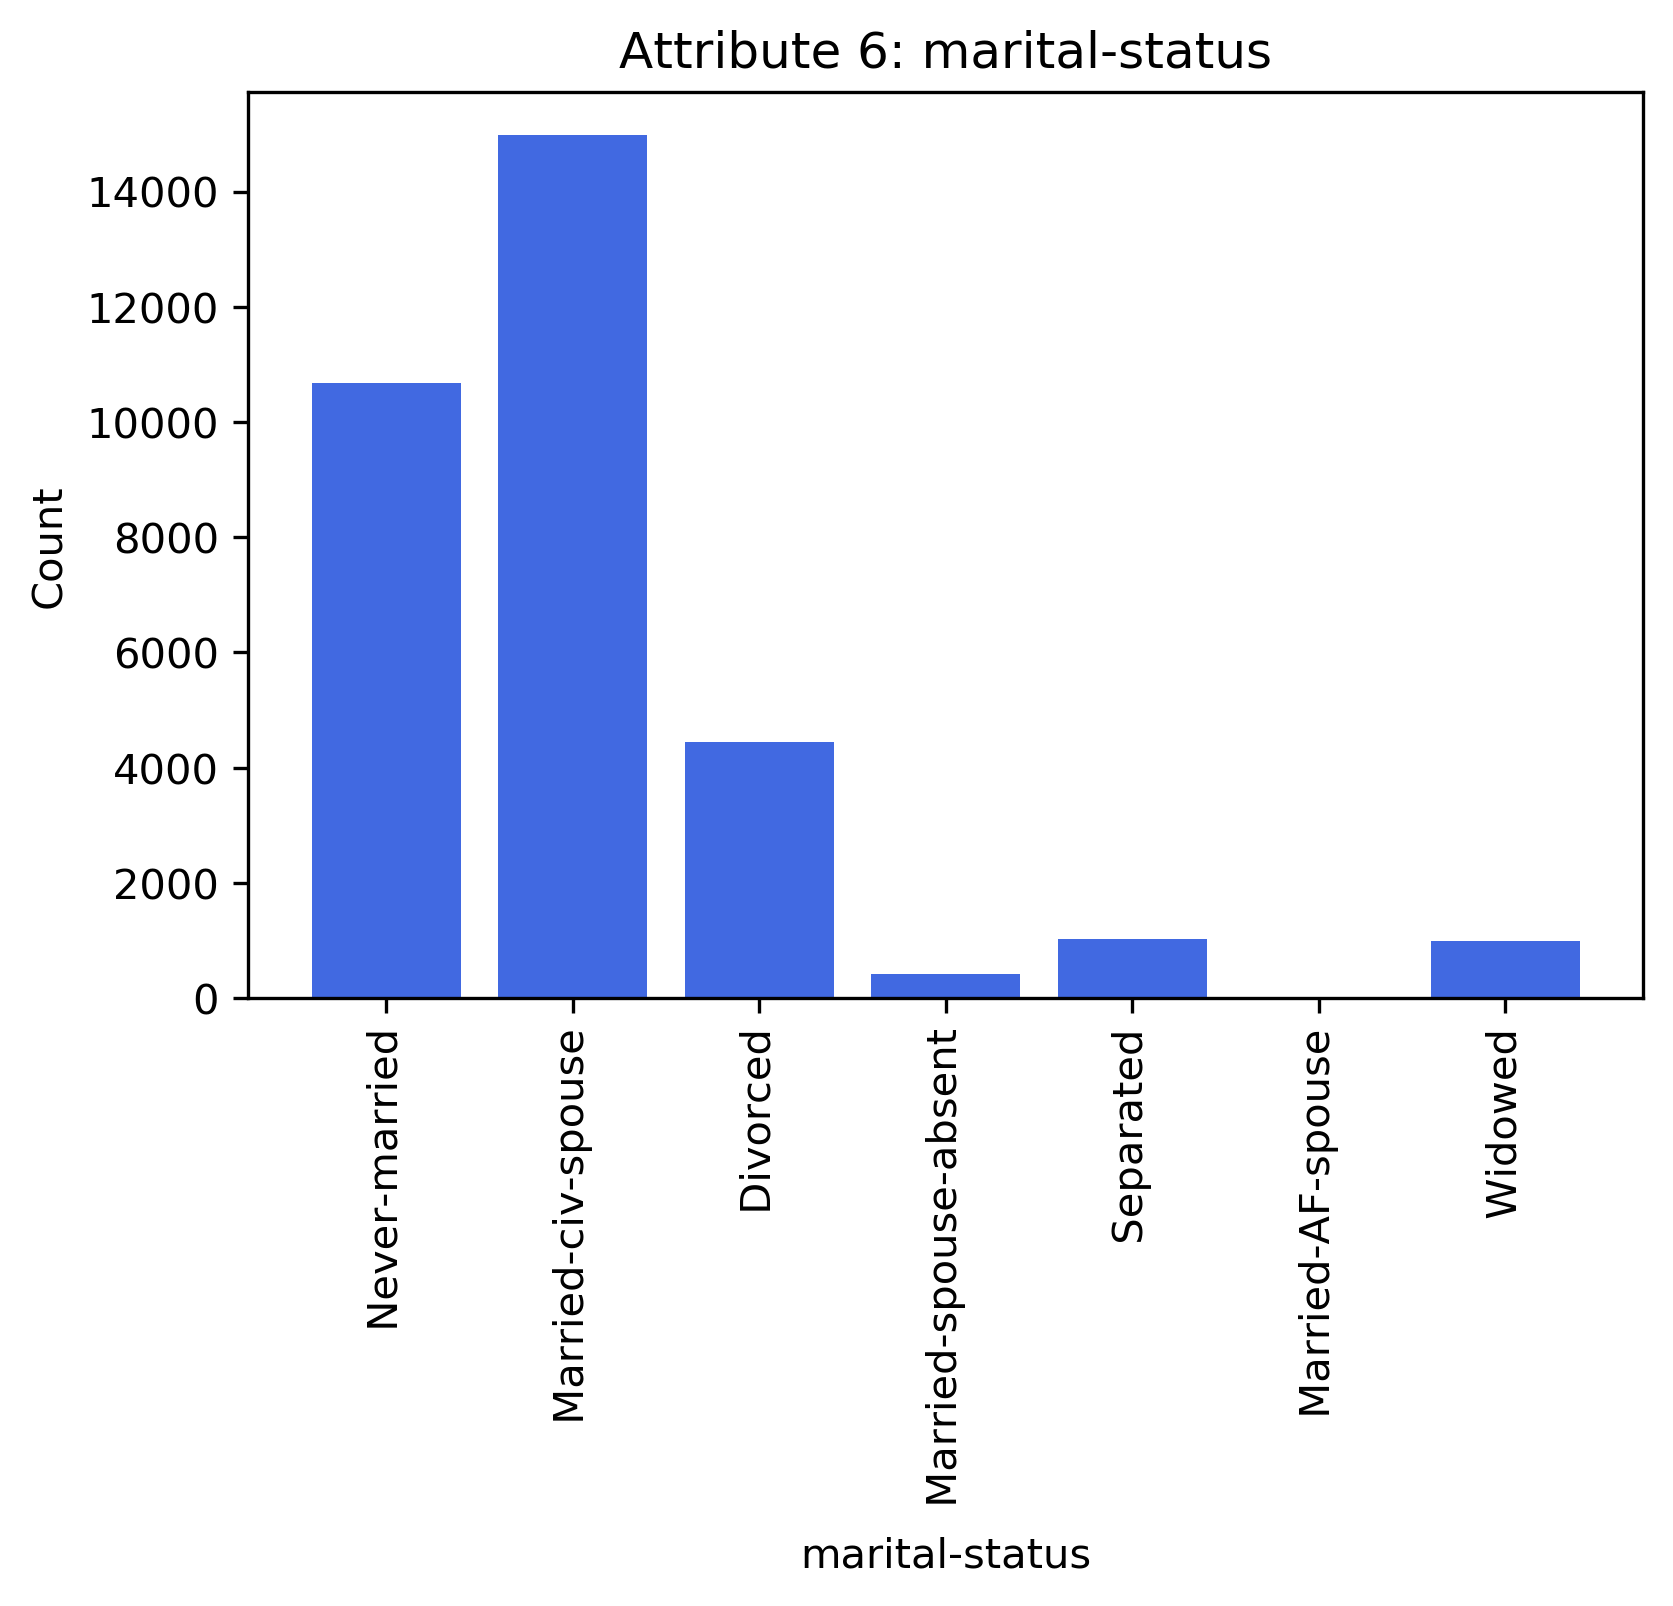
\includegraphics[width=.32\textwidth]{images/5.png}
			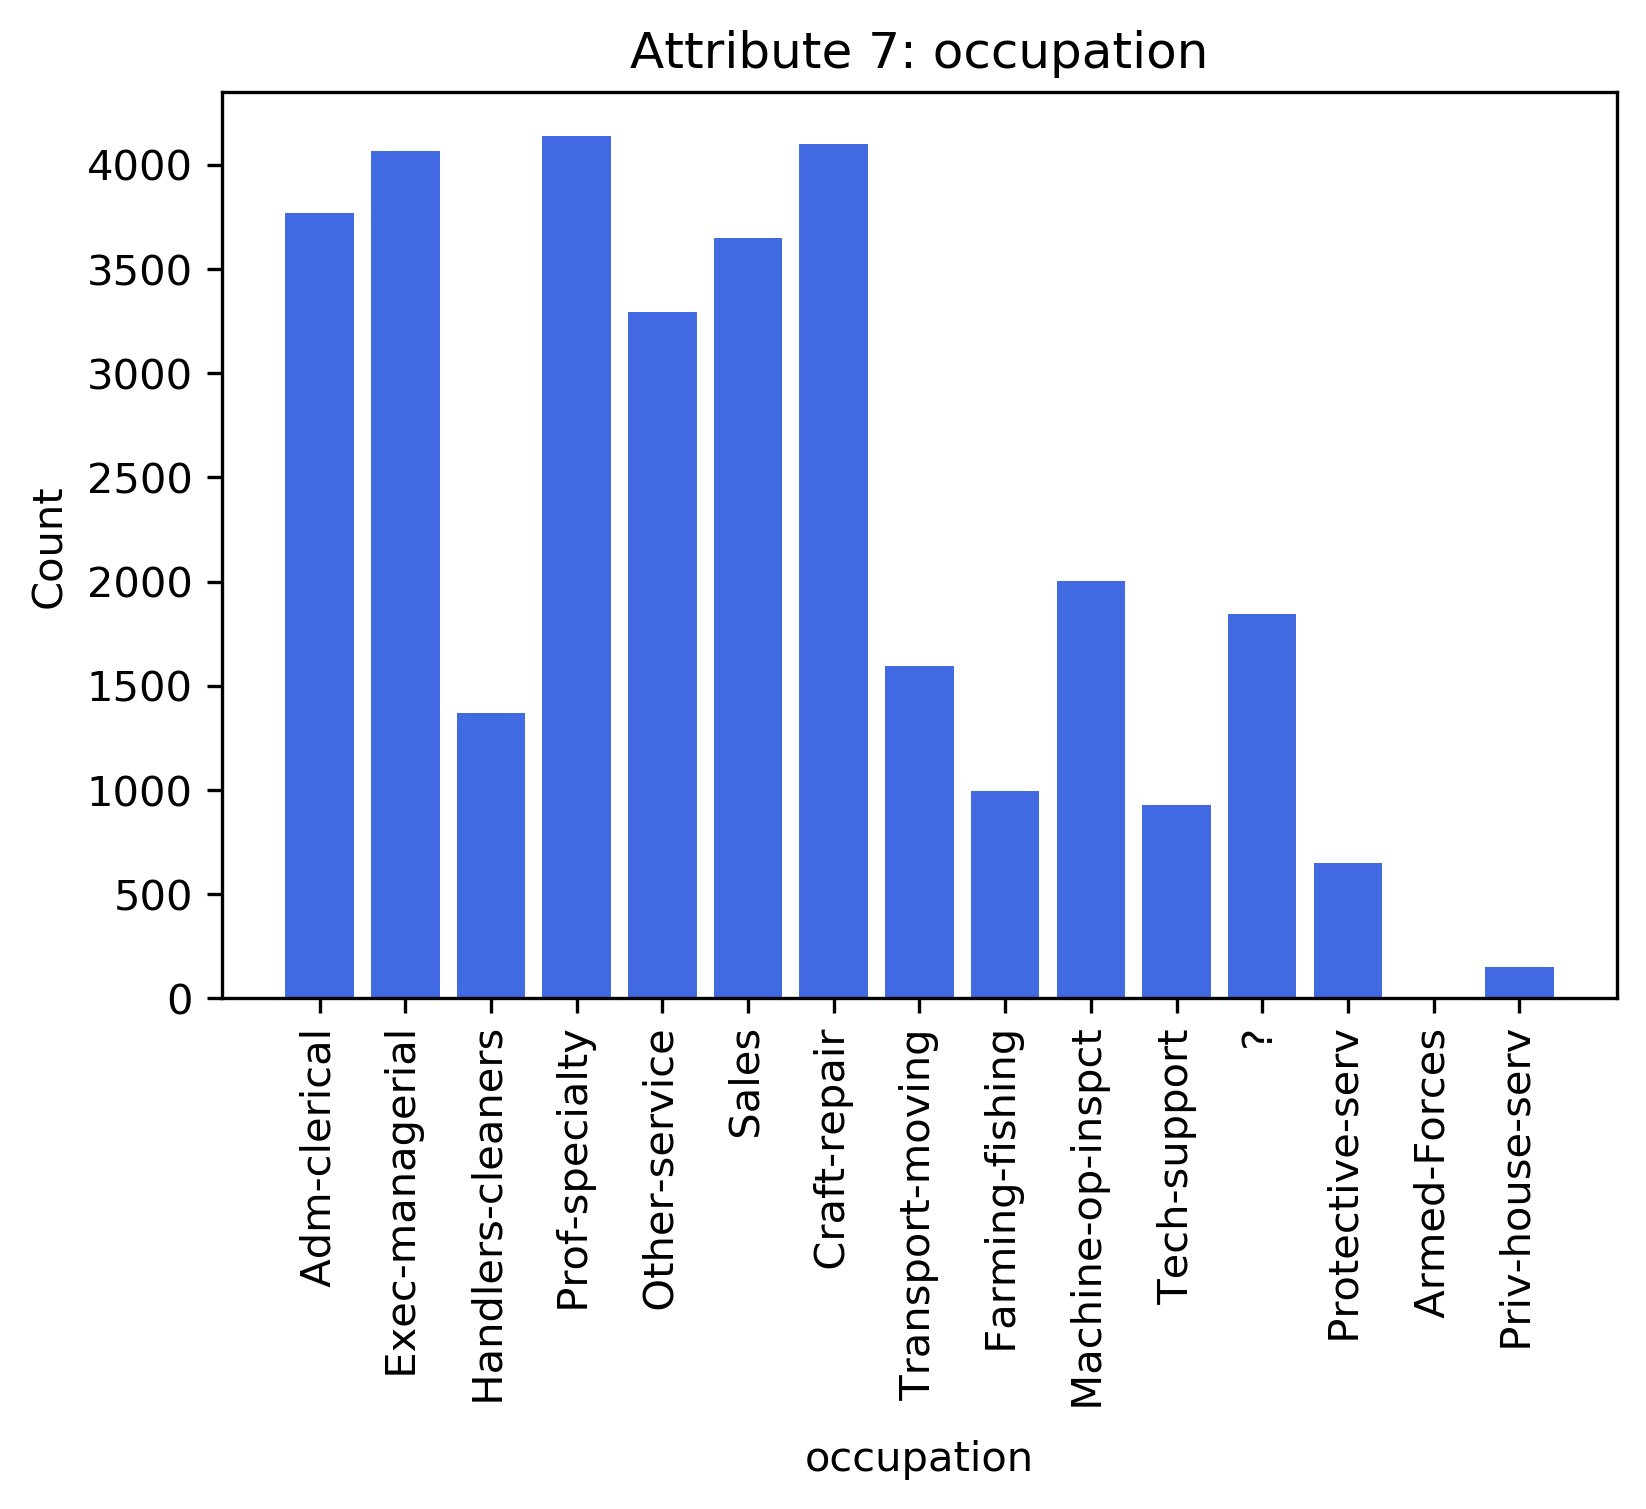
\includegraphics[width=.32\textwidth]{images/6.png}
			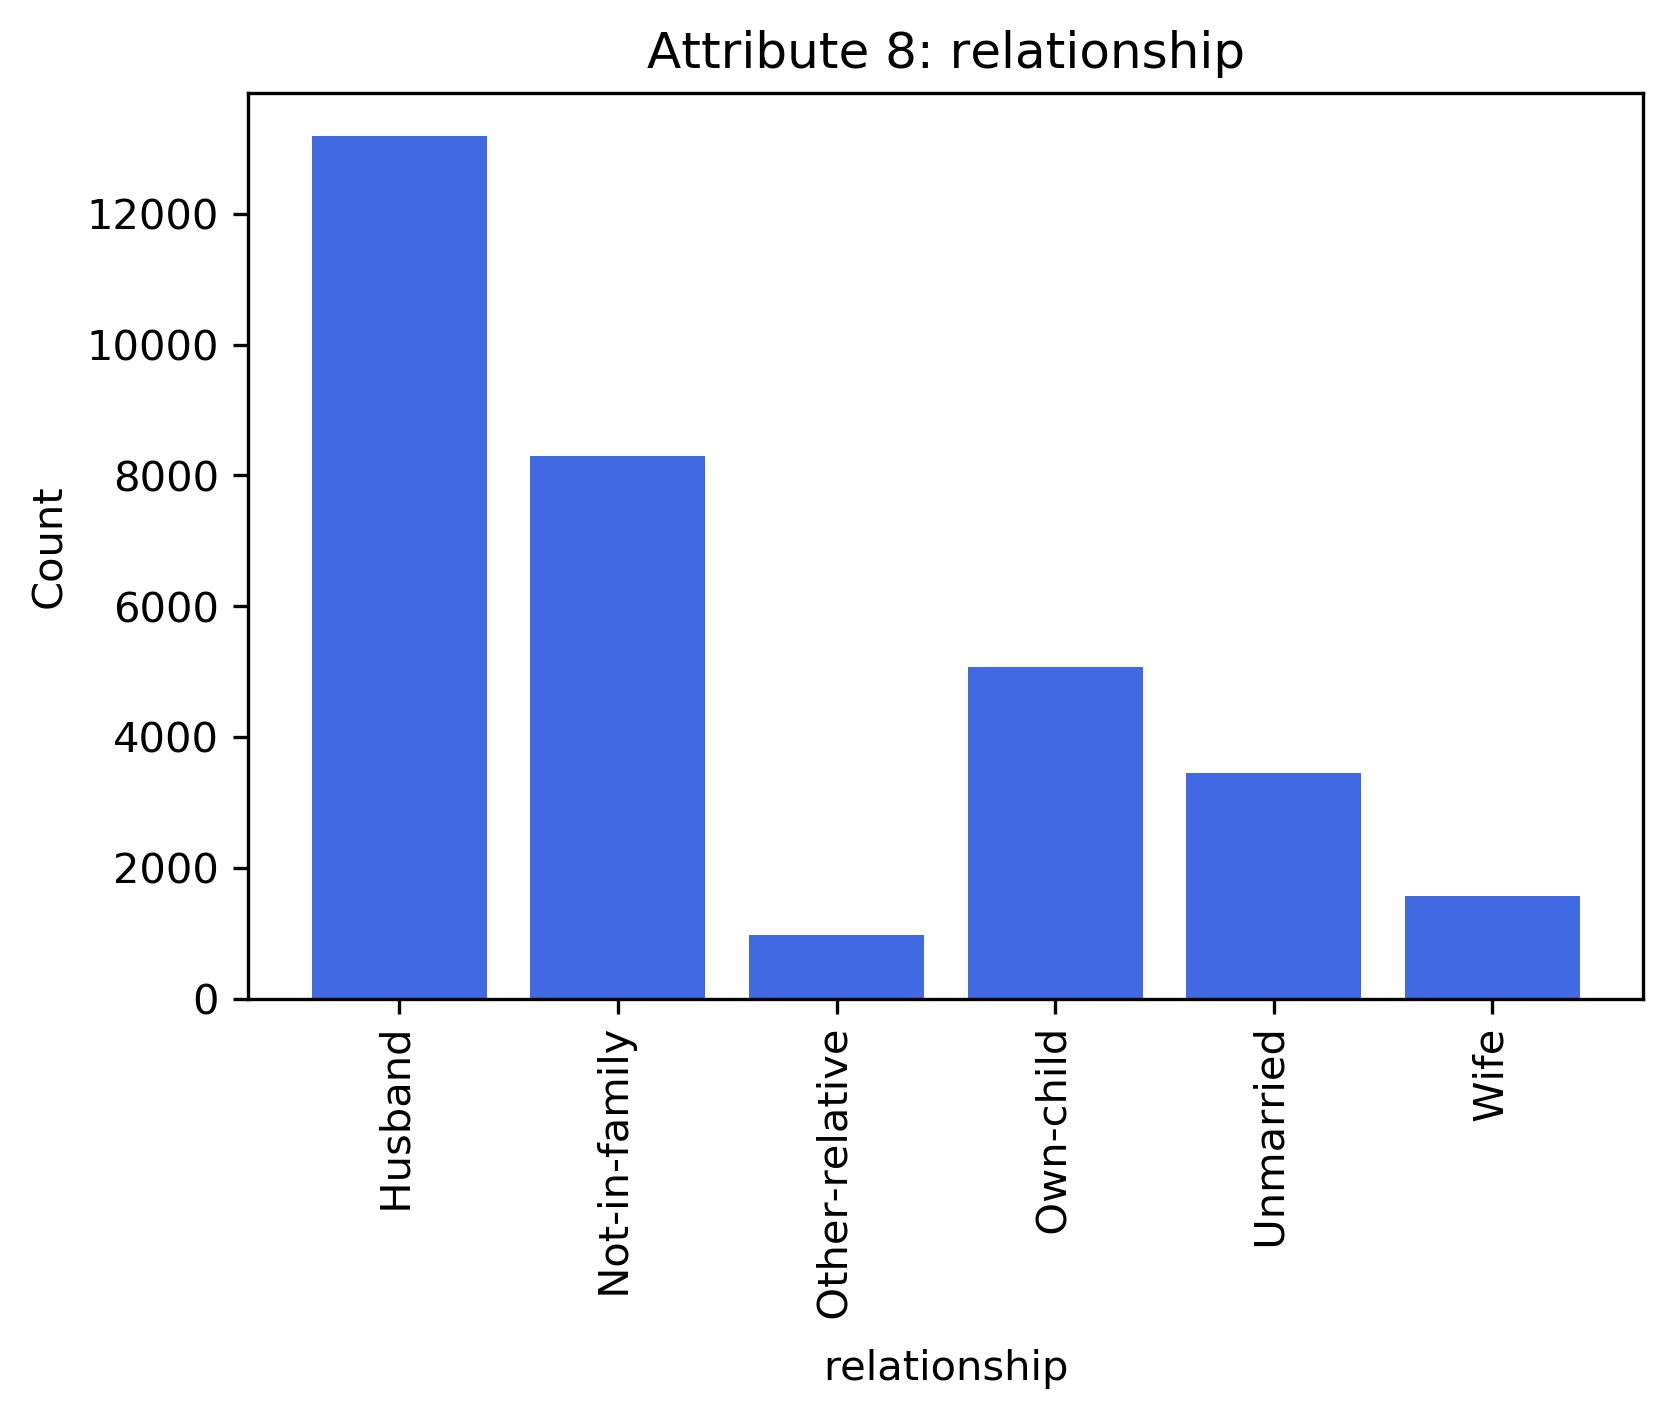
\includegraphics[width=.32\textwidth]{images/7.png}		
			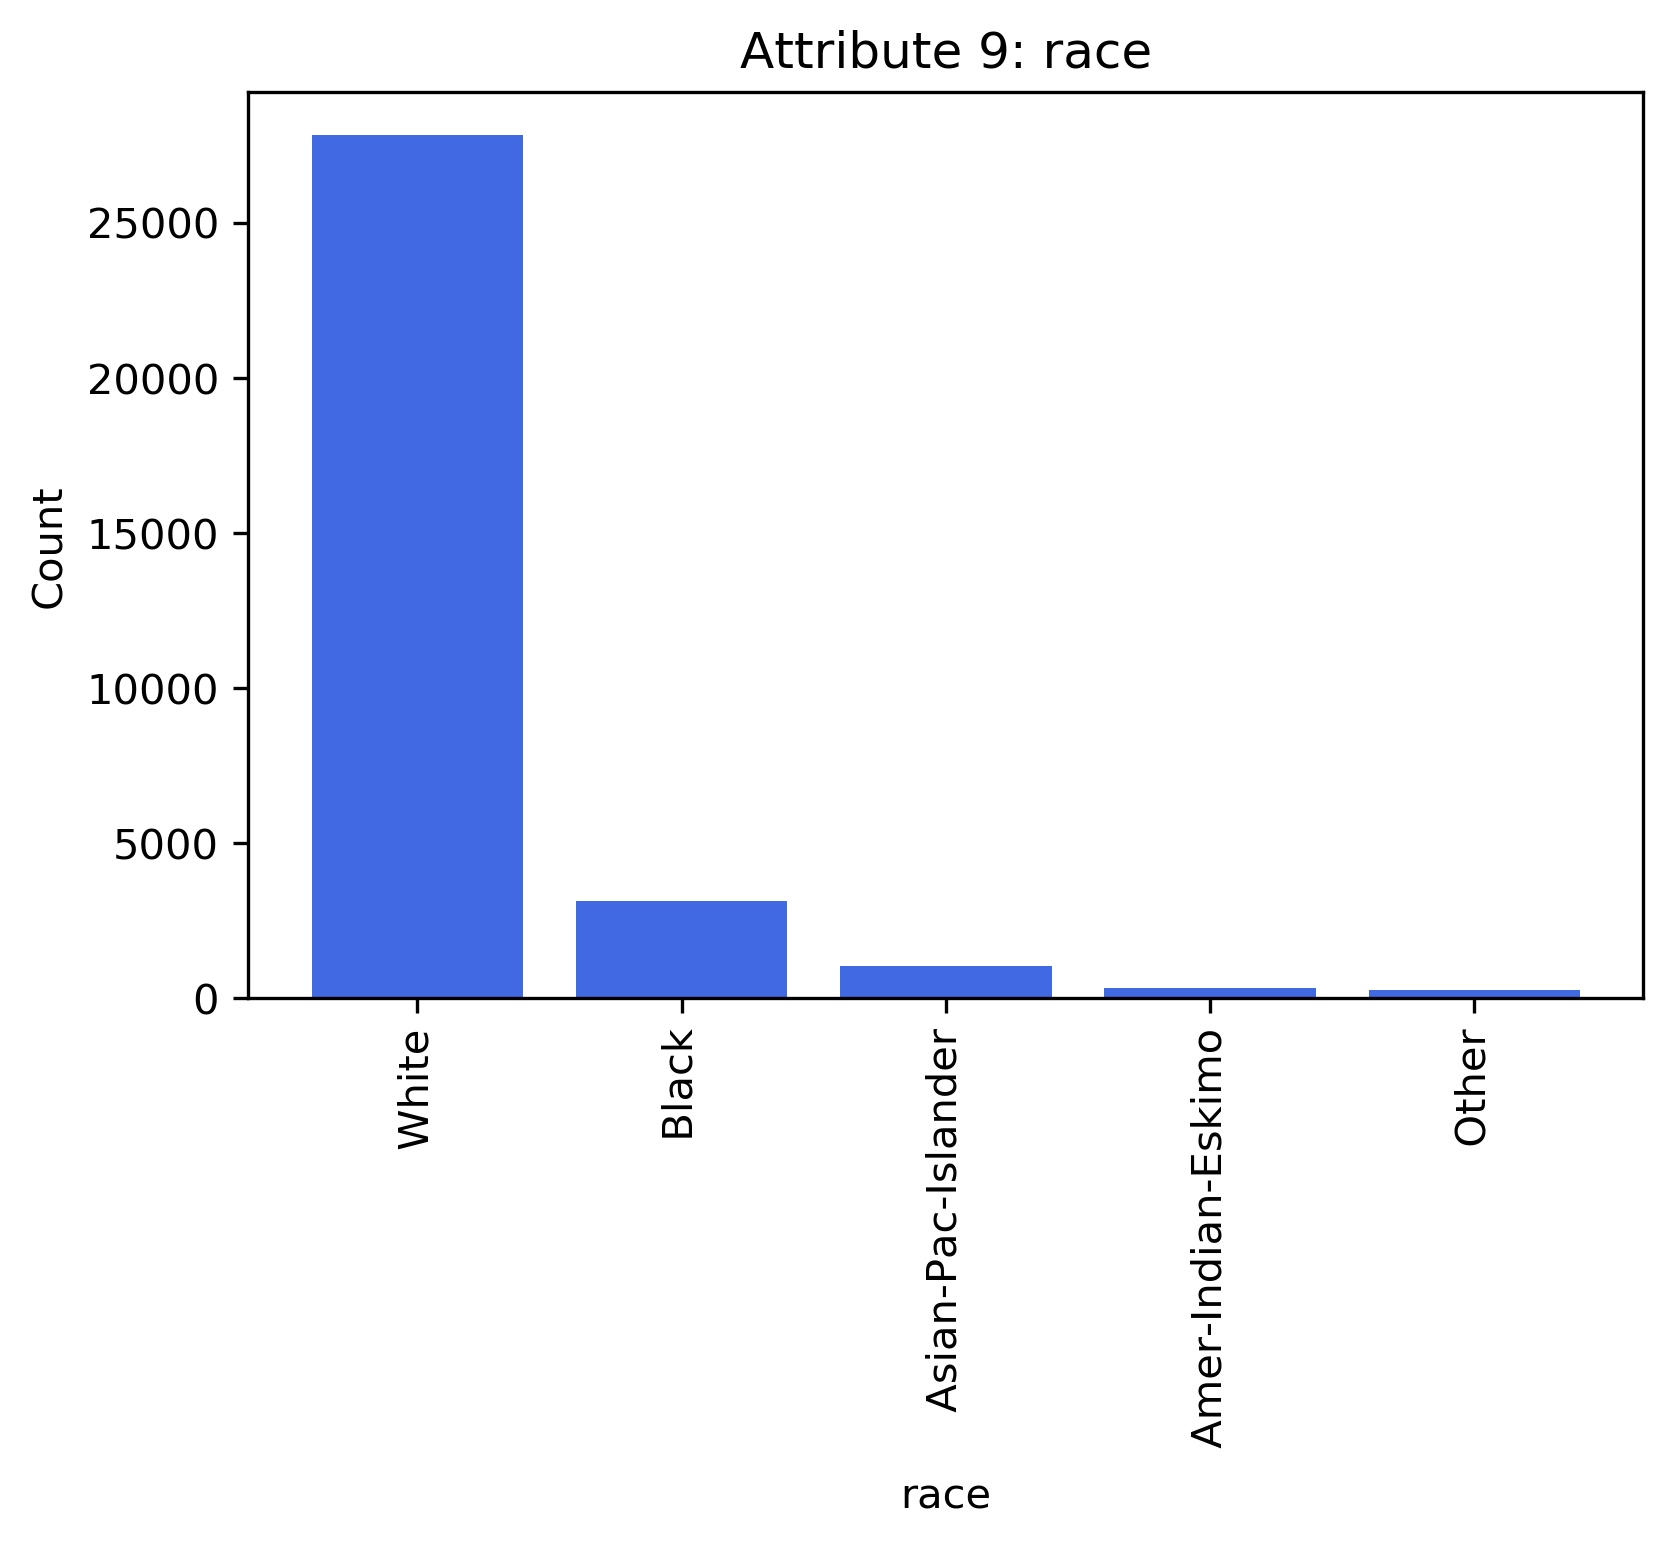
\includegraphics[width=.32\textwidth]{images/8.png}
			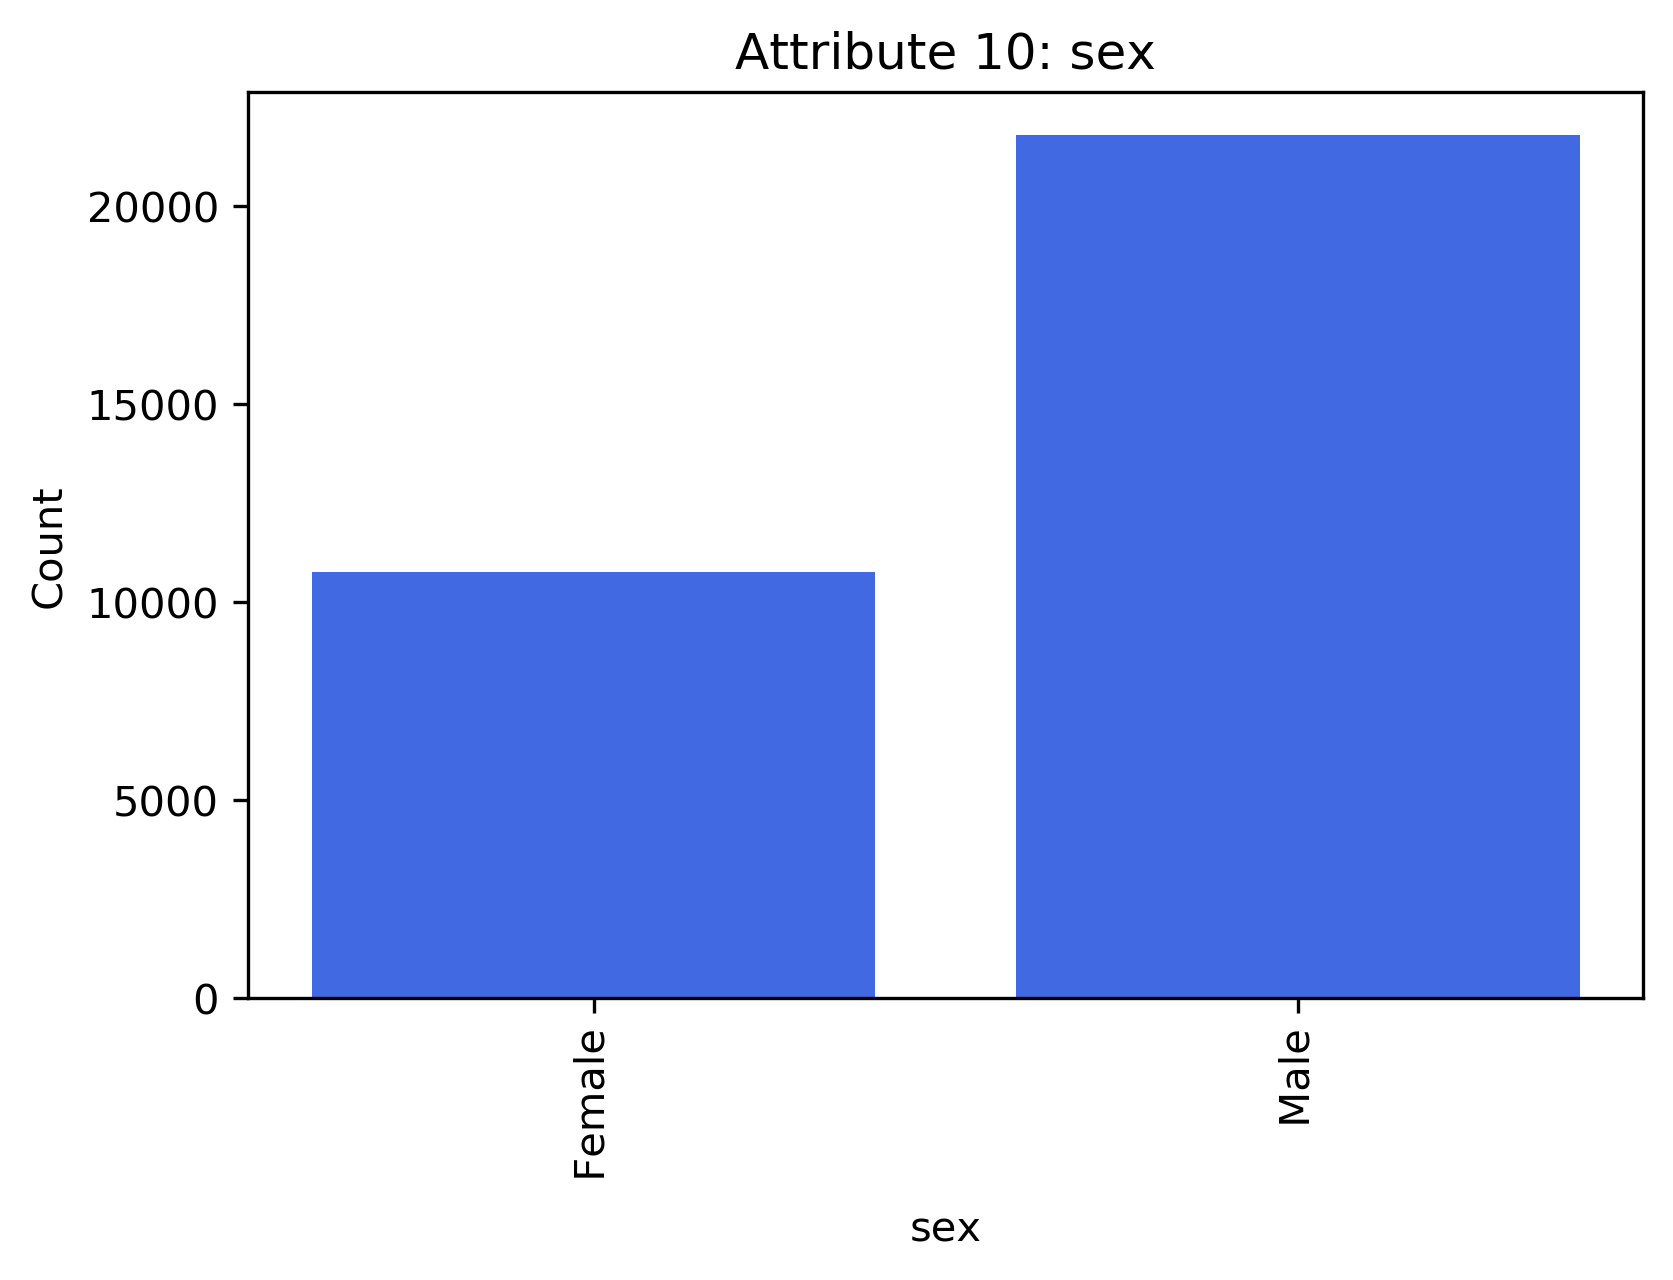
\includegraphics[width=.32\textwidth]{images/9.png}
			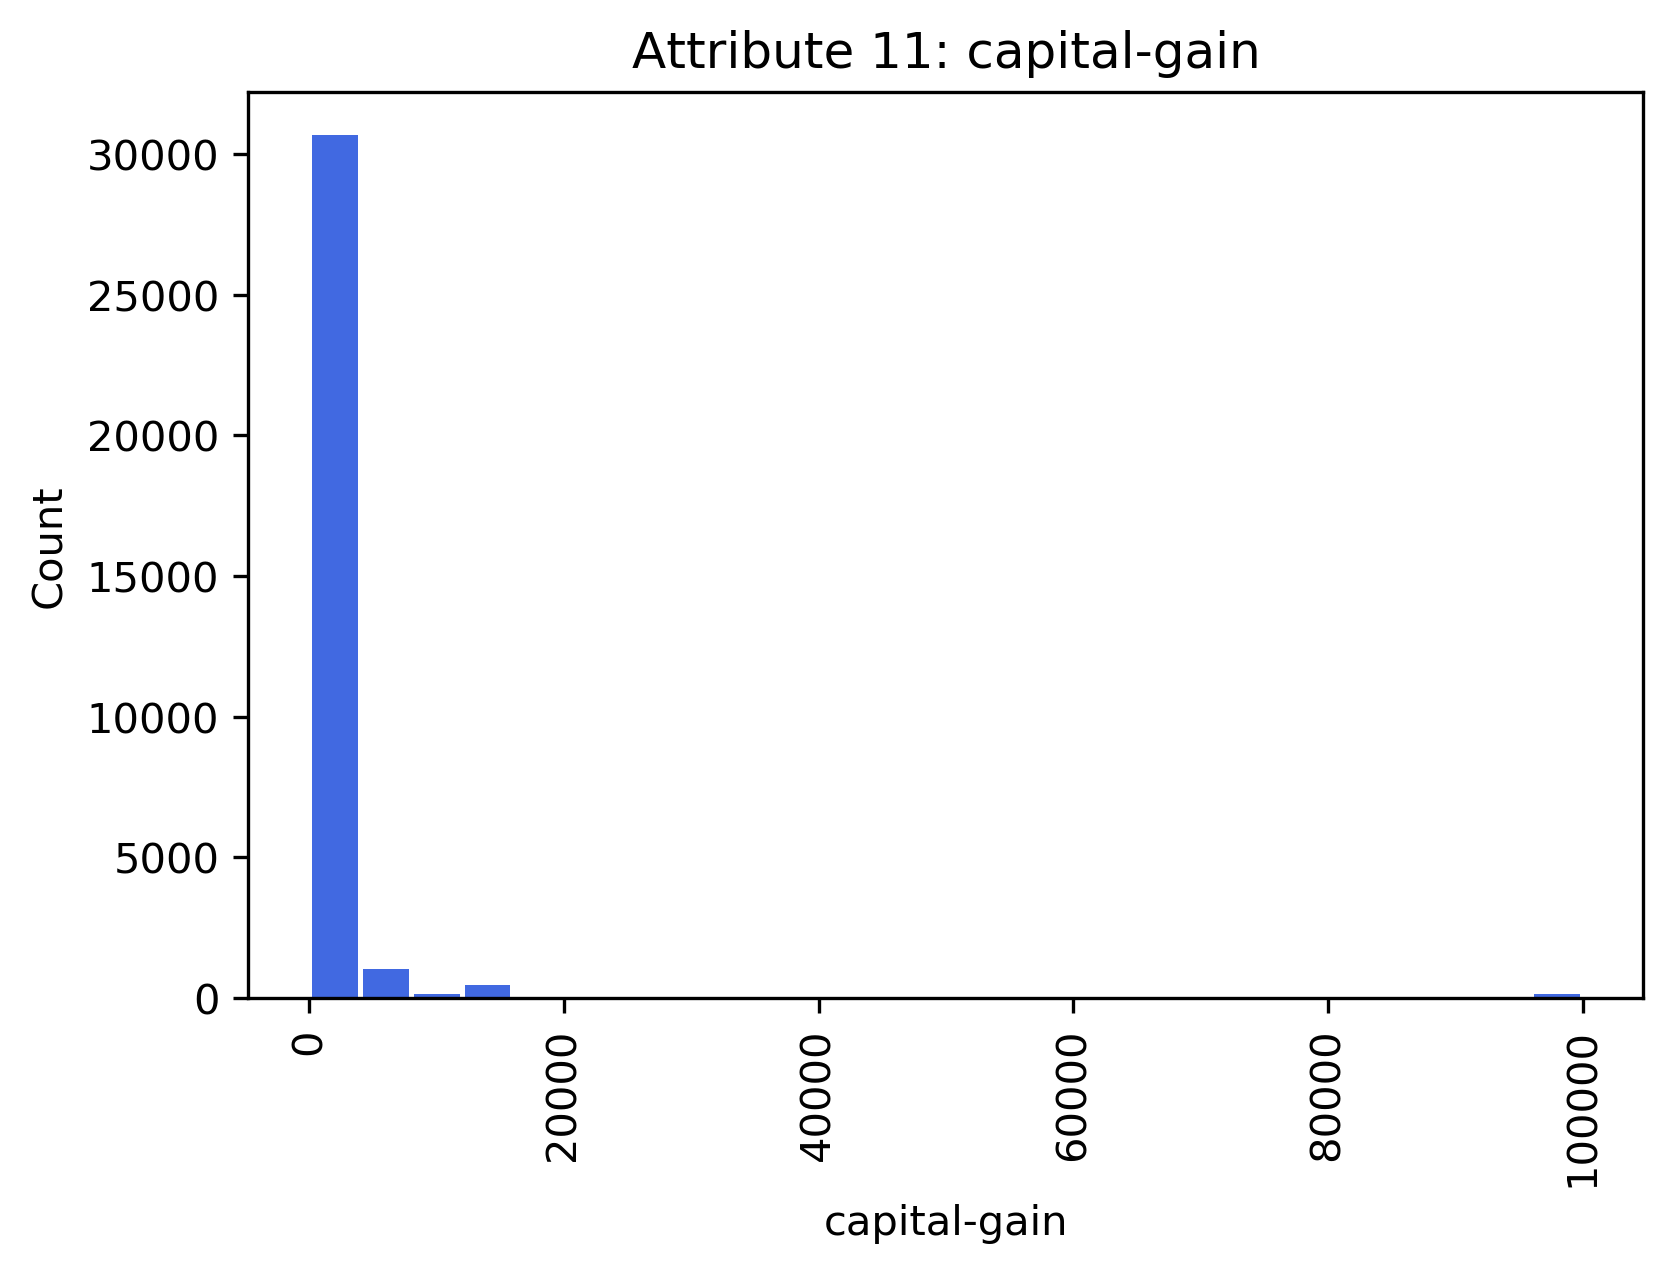
\includegraphics[width=.32\textwidth]{images/10.png}
			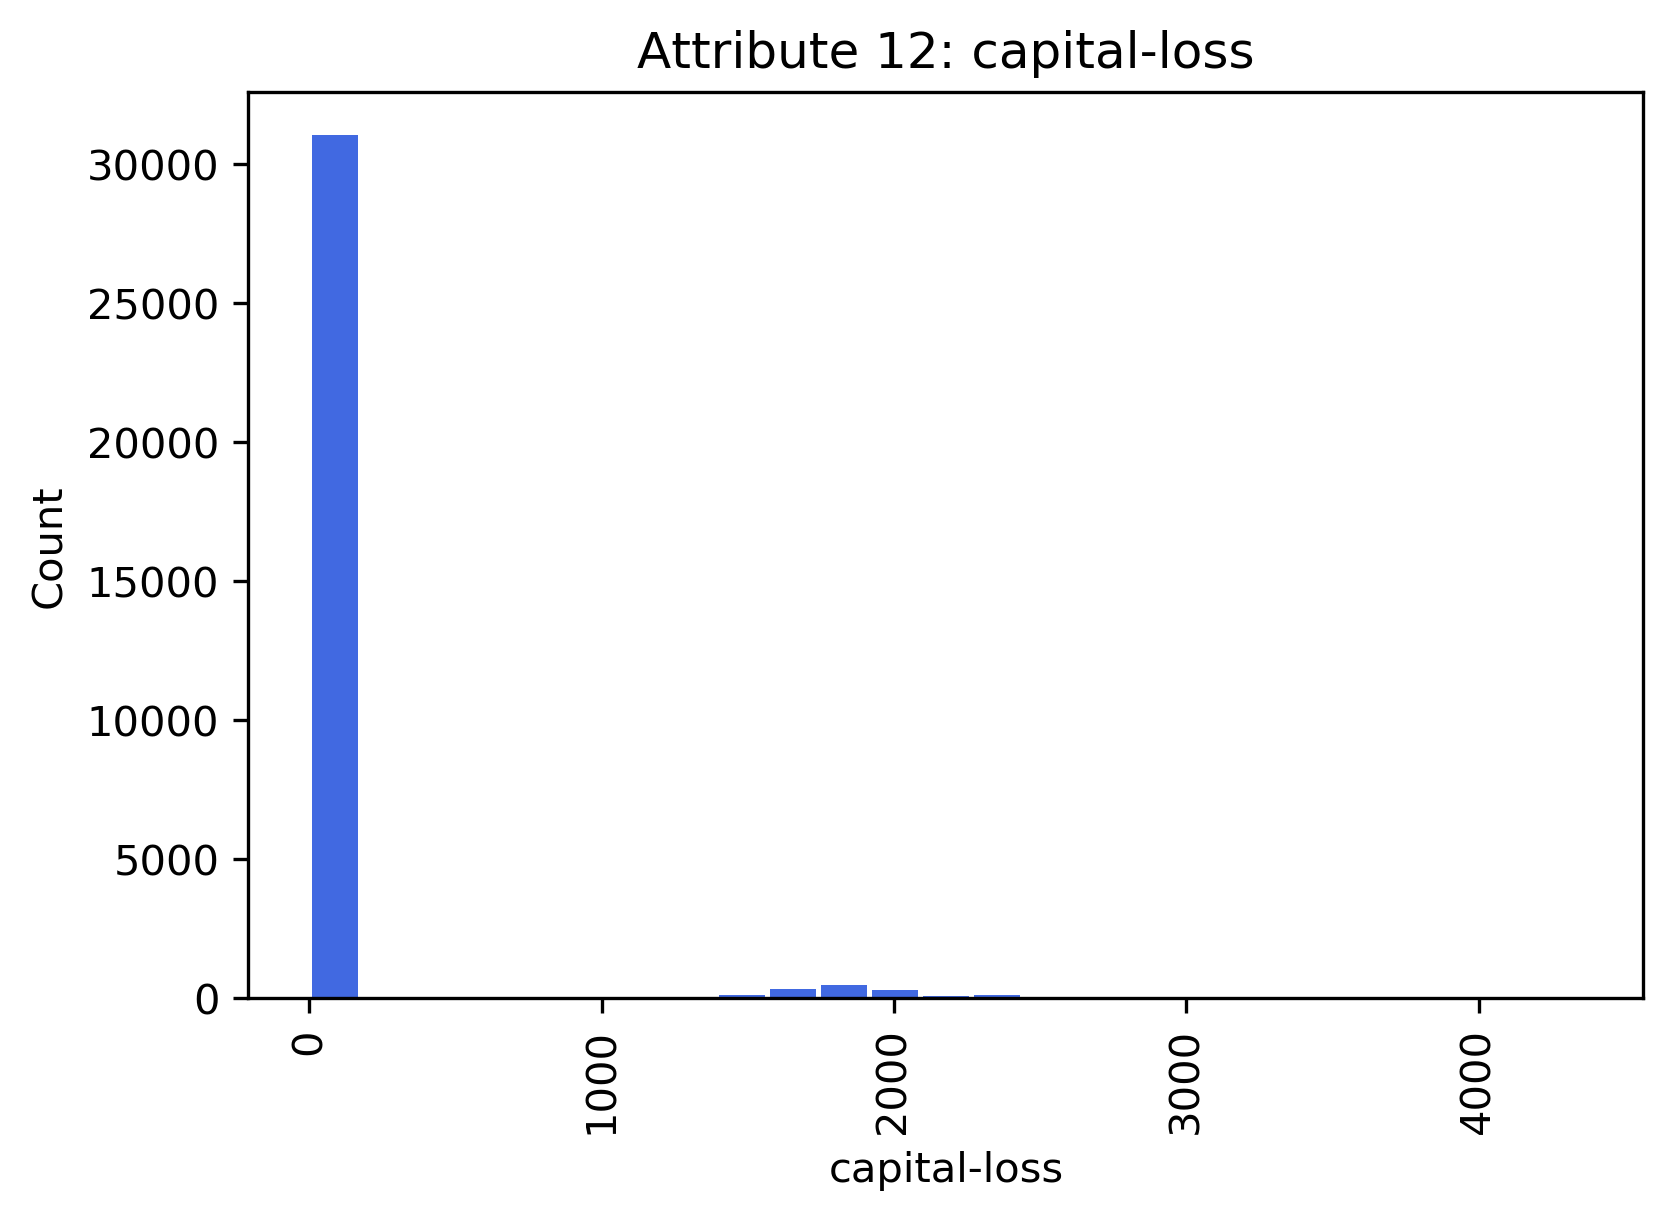
\includegraphics[width=.32\textwidth]{images/11.png}		
			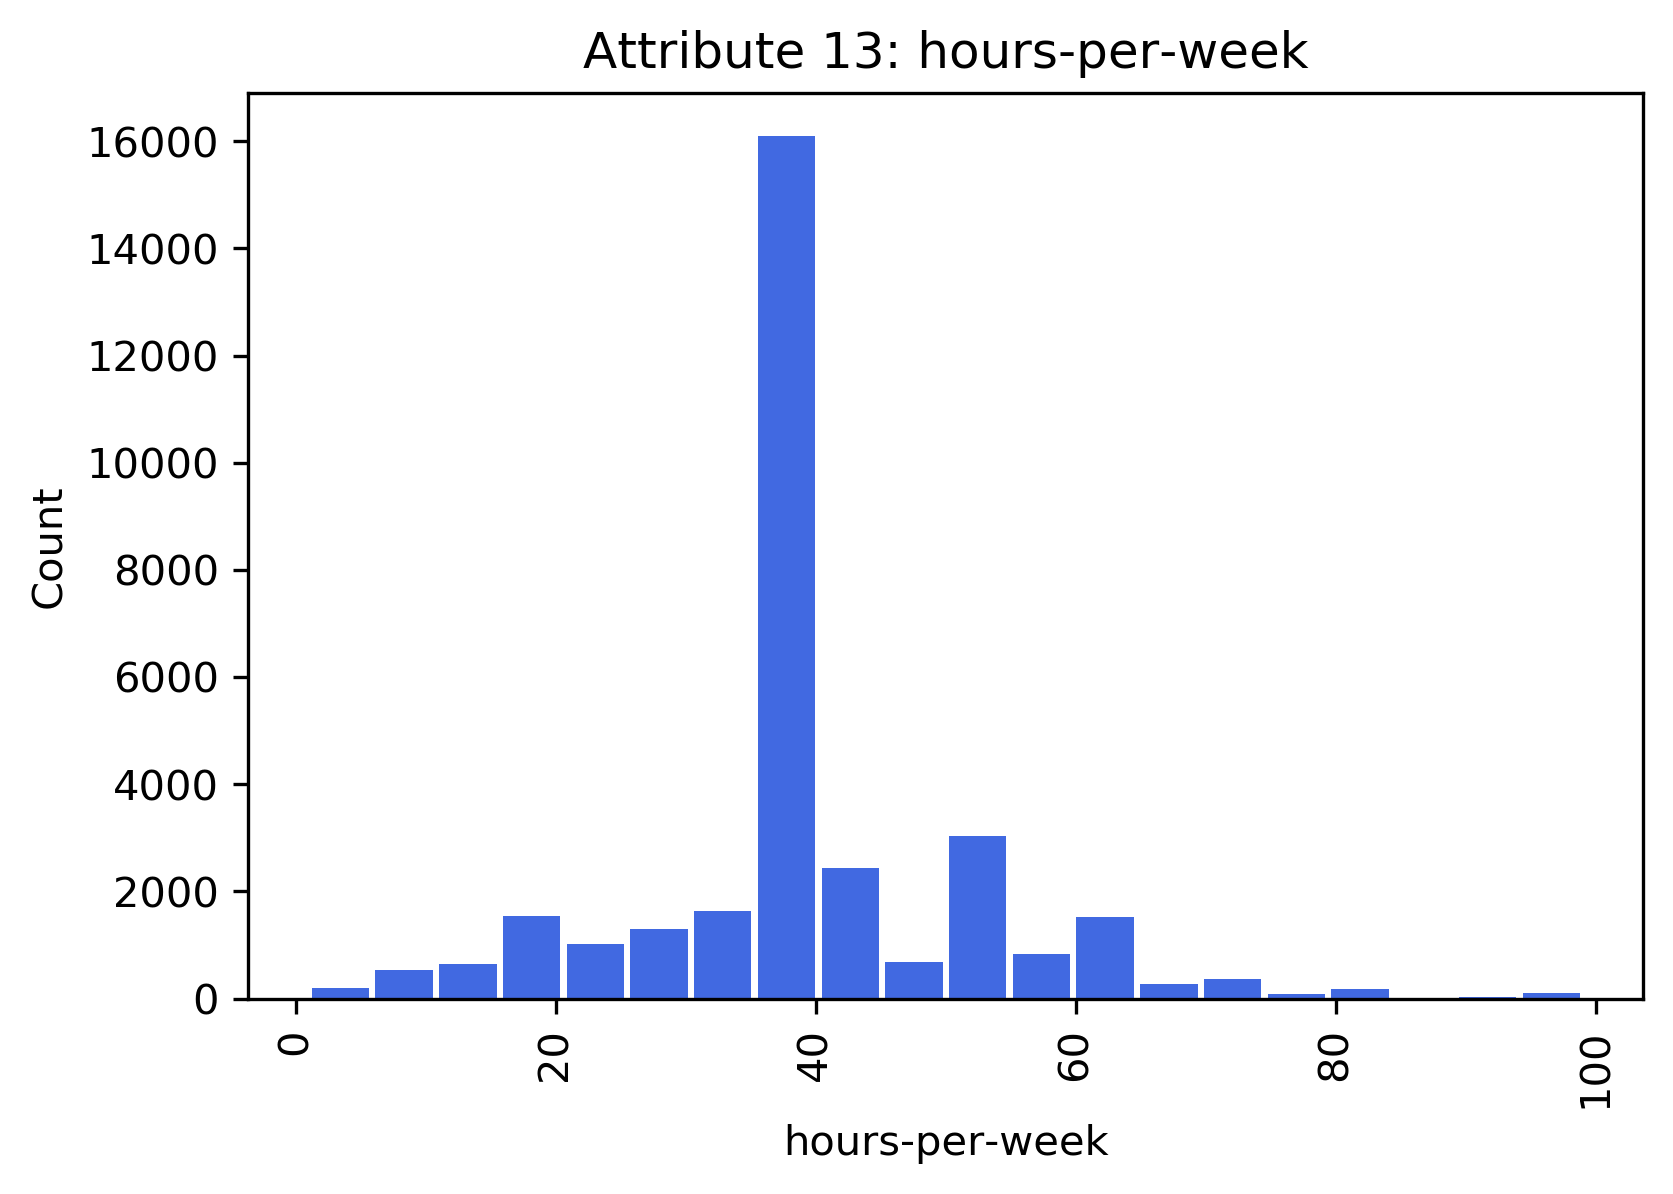
\includegraphics[width=.4\textwidth]{images/12.png}		
			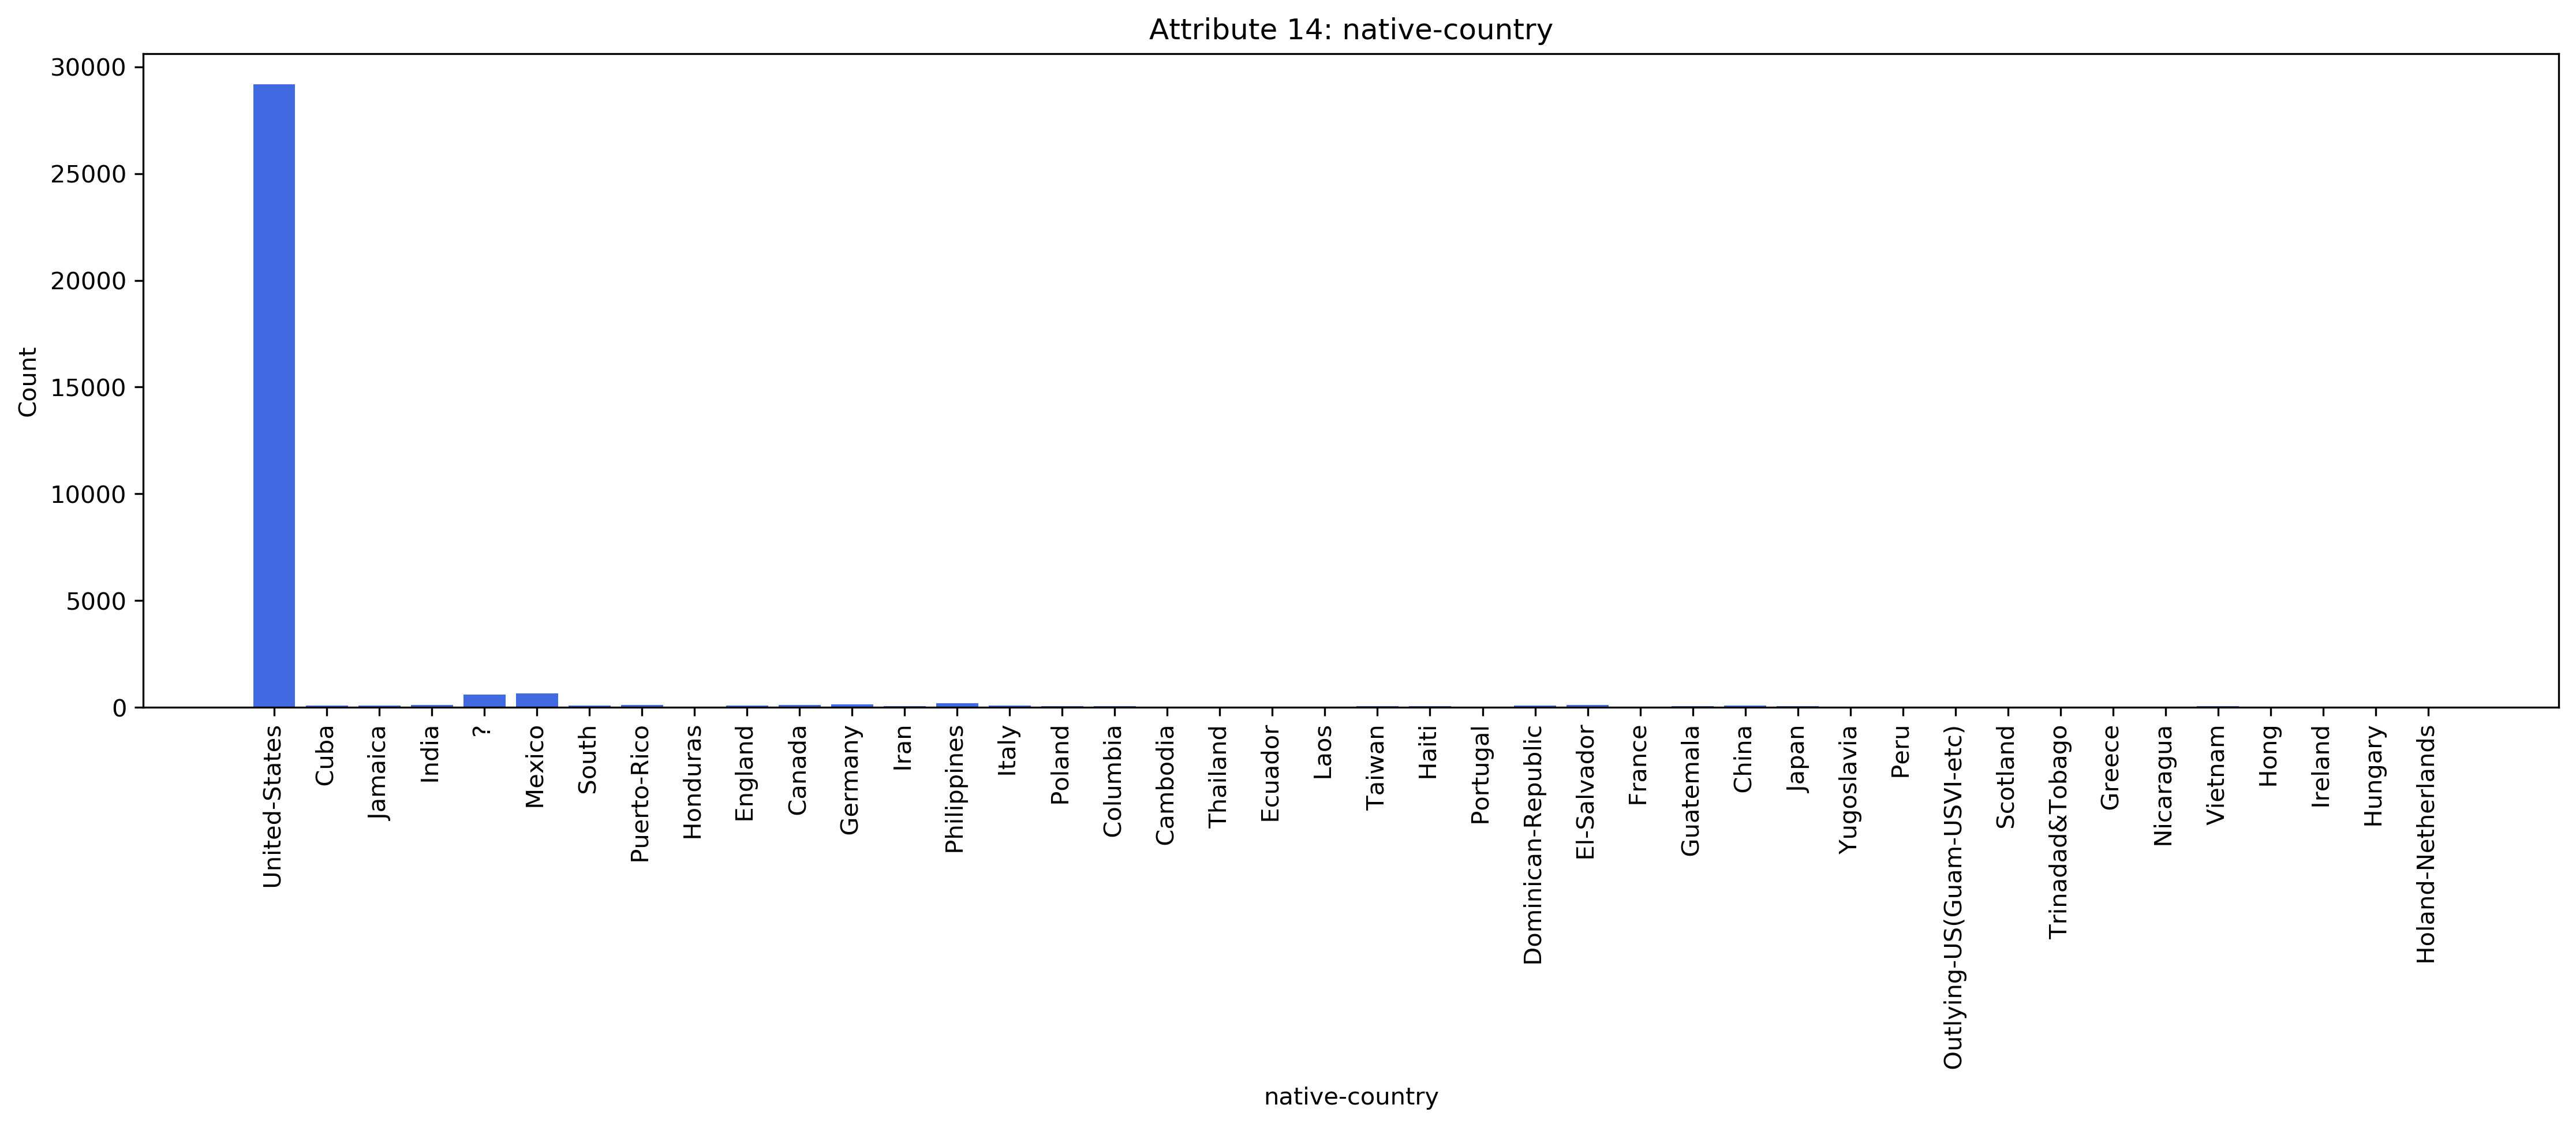
\includegraphics[width=.58\textwidth]{images/13.png}		

		\end{center}
		
		Approximately $7\%$ of the instances (rows) in the unprocessed data set had information missing (indicated by '?' in the histograms). There are a few possible approaches to dealing with this situation, such as approximating values based on similarly close point observations. Though to simplify the data cleaning, we simply remove all cases where data was missing for any specific person. This meant that from the original $ 32561 $ people in the training data we only utilized $ 30162 $ of these, and of the $ 16281 $ people in the test set, we used $ 15060 $.
		
		All categorical data was then converted into a numerical representation allowing for easier manipulation of data within the fitted \emph{sklearn} functions.
		
		\newpage
		\subsection{Manipulation}~
		We decided to use four transformations of the data set: original, standardized, feature selected, and principle component analysis.
		\subsubsection{Original}~
		
			The data used here is directly translated from the original data-set. Converting all catagorical data to numerical values. No other processing has been done to alter the data in a way making it difficult to reproduce the original.
		
		\begin{itemize}
			\item 	Benefits: 
			\begin{itemize}
				\item Simplicity of set-up in preperation for actual "data-mining" techinques to be applied
				\item No information loss
			\end{itemize}
			\item  	Disadvantages: 
			\begin{itemize}
				\item Does not deal well with outlier cases
				\item Numerical errors are more likely to occur as some numbers become very large
				\item We are still dealing with all of the data attributes, causing fitting algorithms to be slowed
			\end{itemize}
		\end{itemize}
		
		\subsubsection{Standardized}~
		
		Standardization of the data set is used to help fix some common problems that may arise when dealing with the original data. The idea of standardization is to shift the data so that it has a mean of 0 and a standard deviation of 1. Thereby minimizing the variance that exists within the unscaled data and dealing with issues that arise from relatively large numbers. It also scales values down to a manageable size limiting the possibility of overflow.\\\\
		Standardization Formula: 
		
		\begin{equation}
		 X_{ij} = \dfrac{X_{ij}- E(X_j)}{\sqrt{V(X_j)}}
		\end{equation}
		 $ i \times j := $ row $ \times $ column indices.\\ $ E(X_j),V(X_j) := $ expectation and variance of $ Xj $
		\begin{itemize}
			\item 	Benefits: 
			\begin{itemize}
				\item Outliers will not have a large influence on model fits
				\item Risk of numerical overflows is greatly reduced
				\item Data holds a closer representation to a normal distribution (being shifted and scaled down)
			\end{itemize}
			\item  	Disadvantages: 
			\begin{itemize}
				\item We are still dealing with high-dimensional data
				\item Data may not be appropriately represented once standardized (i.e. incorrect distribution assumptions)
			\end{itemize}
		\end{itemize}
			
		\subsubsection{Feature Selection}~

		This data technique is used specifically to reduce the amount of computation time necessary by removing a large number of the attributes. This technique will reduce the space required to store the data as well. When attributes or features are chosen optimally, this will reduce the risk of over-fitting the model by removing all unnecessary collinear terms. Our selected attributes were chosen based off of our observations of the previous histograms and a step based model selection technique based on the full linear model (using both forwards and backwards elimination techniques). We also remove terms that are overrepresented in the data (eg. over $ 92\% $ were from the US). \\
		
		We chose the following attributes:\\ Age, Education, Education-num, Marital-status, Relationship, Sex, Hours-per-week.\\
		
		The following histograms indicate people who fall under the '$>50000 USD$' class (green), all sampled people (blue), and people who fall under the '$\le50000 USD$' class (red). Only the histograms for education, relationship, and sex are shown as examples of the varying attributes of people in different classes.
		
		\begin{center}
			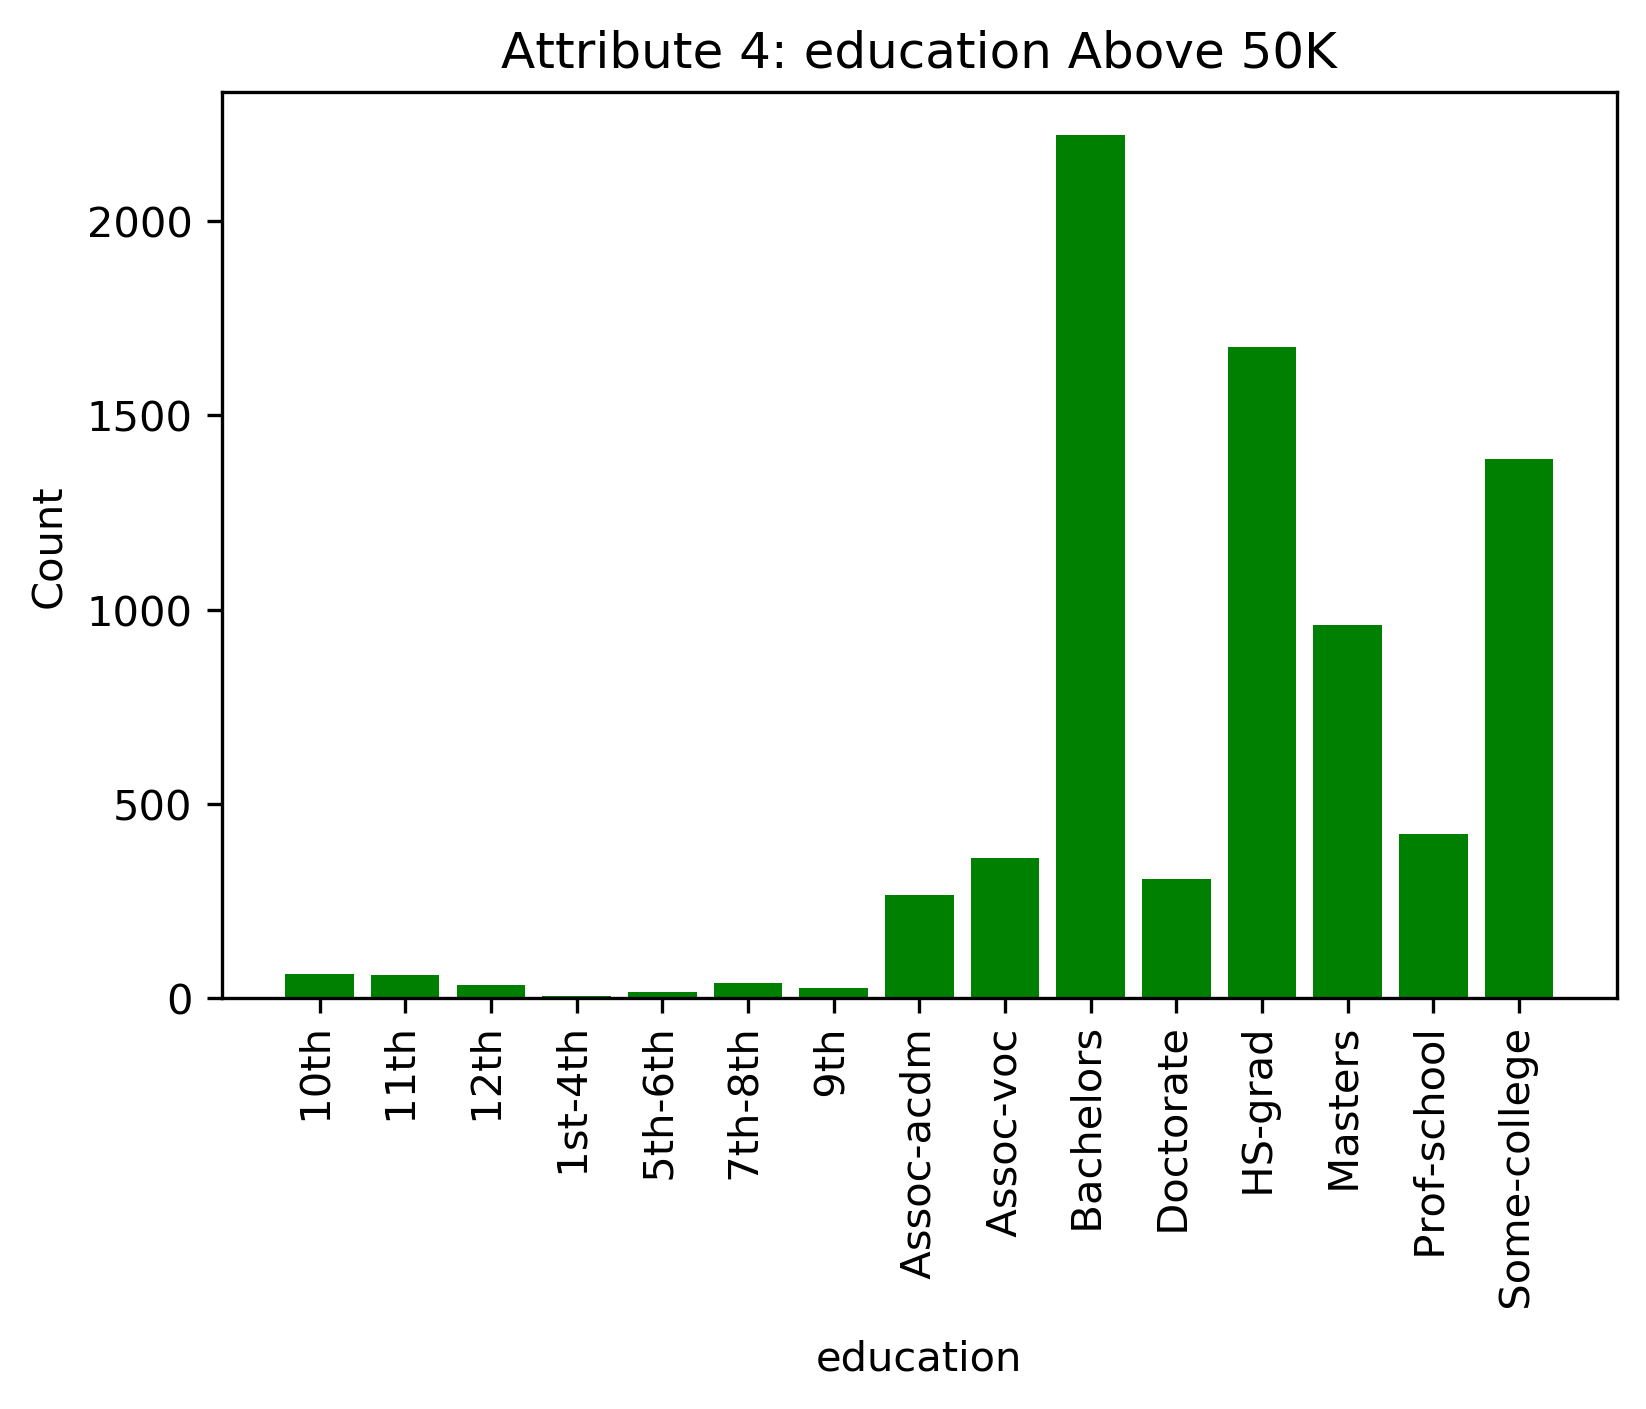
\includegraphics[width=.29\textwidth]{images/3above.png}
			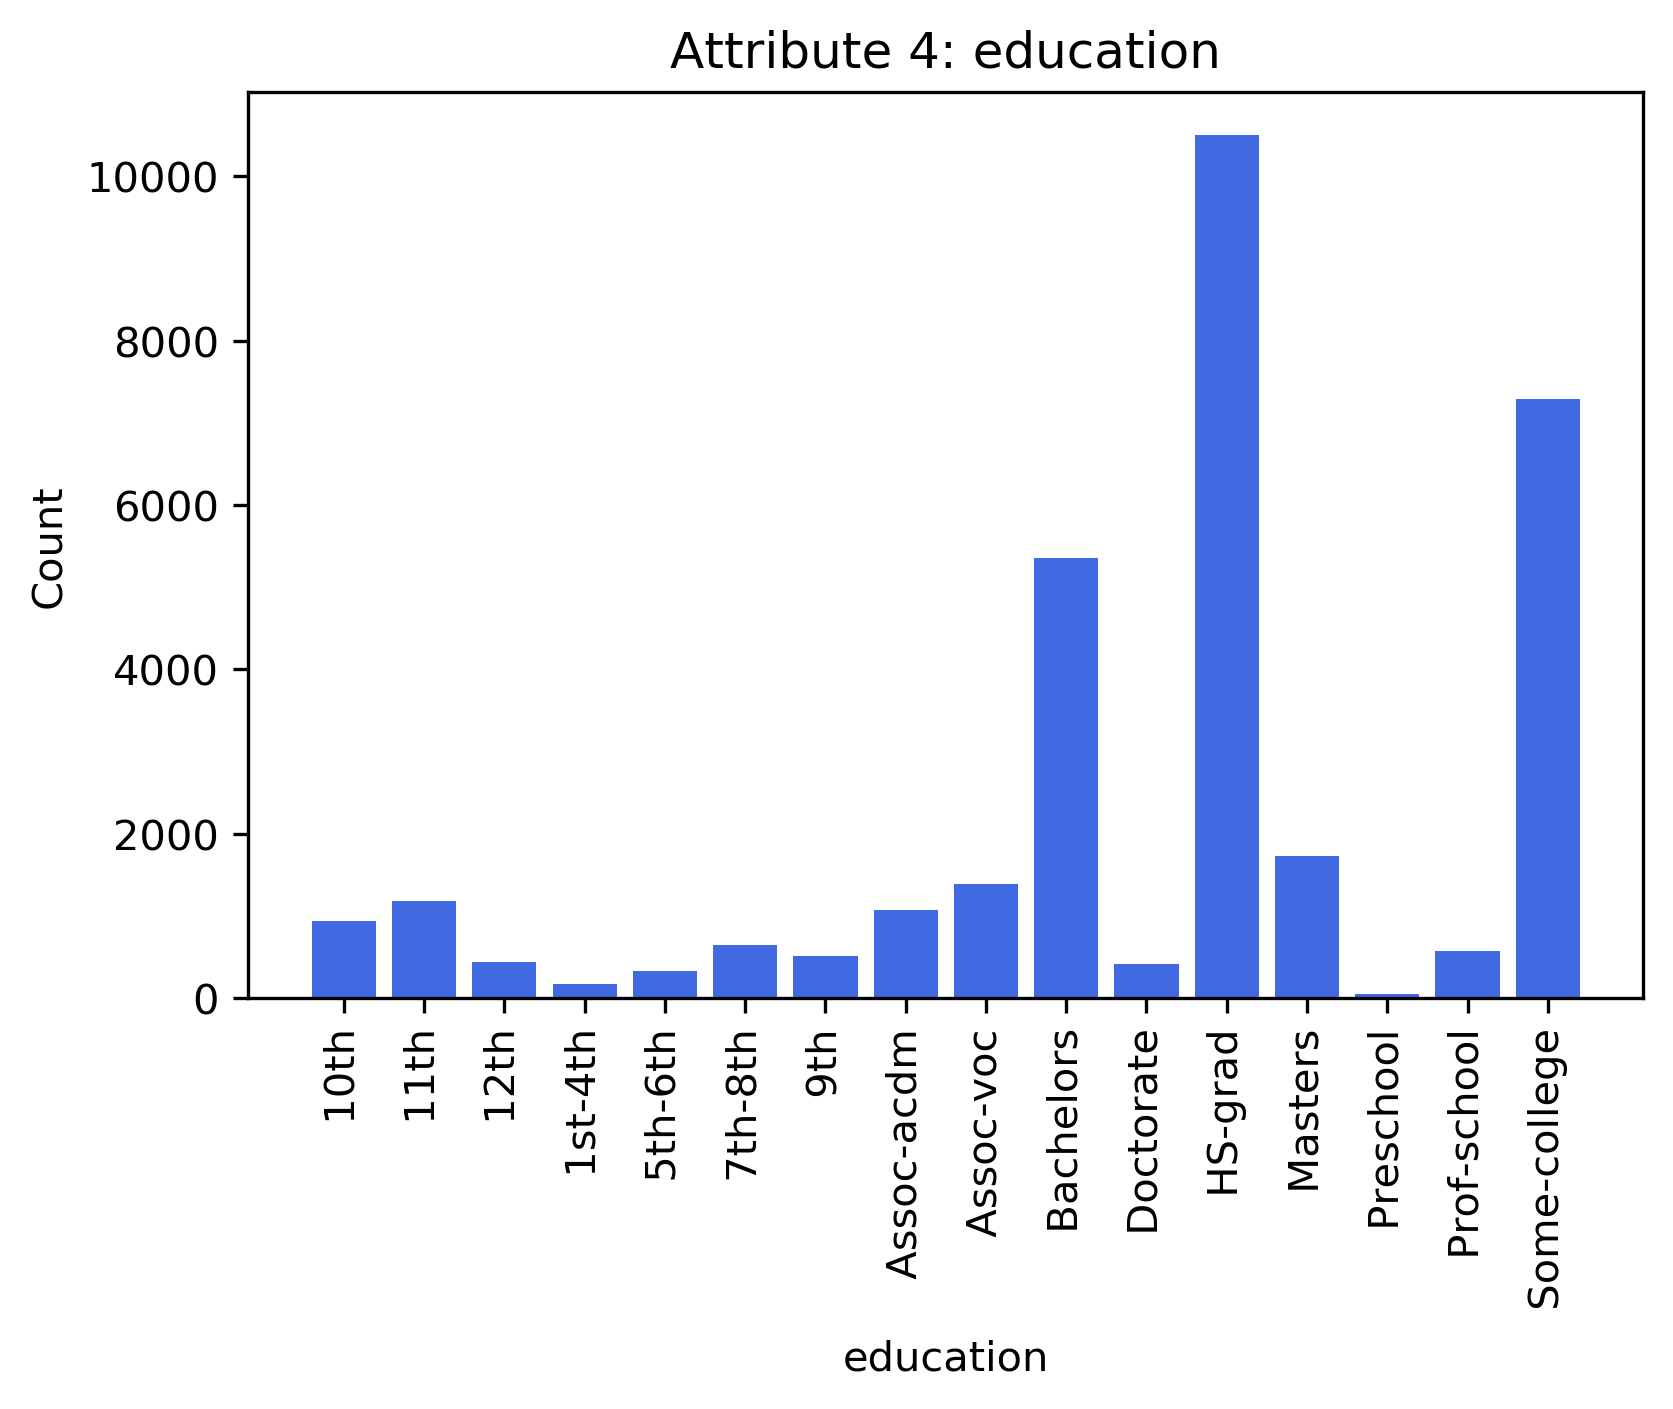
\includegraphics[width=.4\textwidth]{images/3.png}
			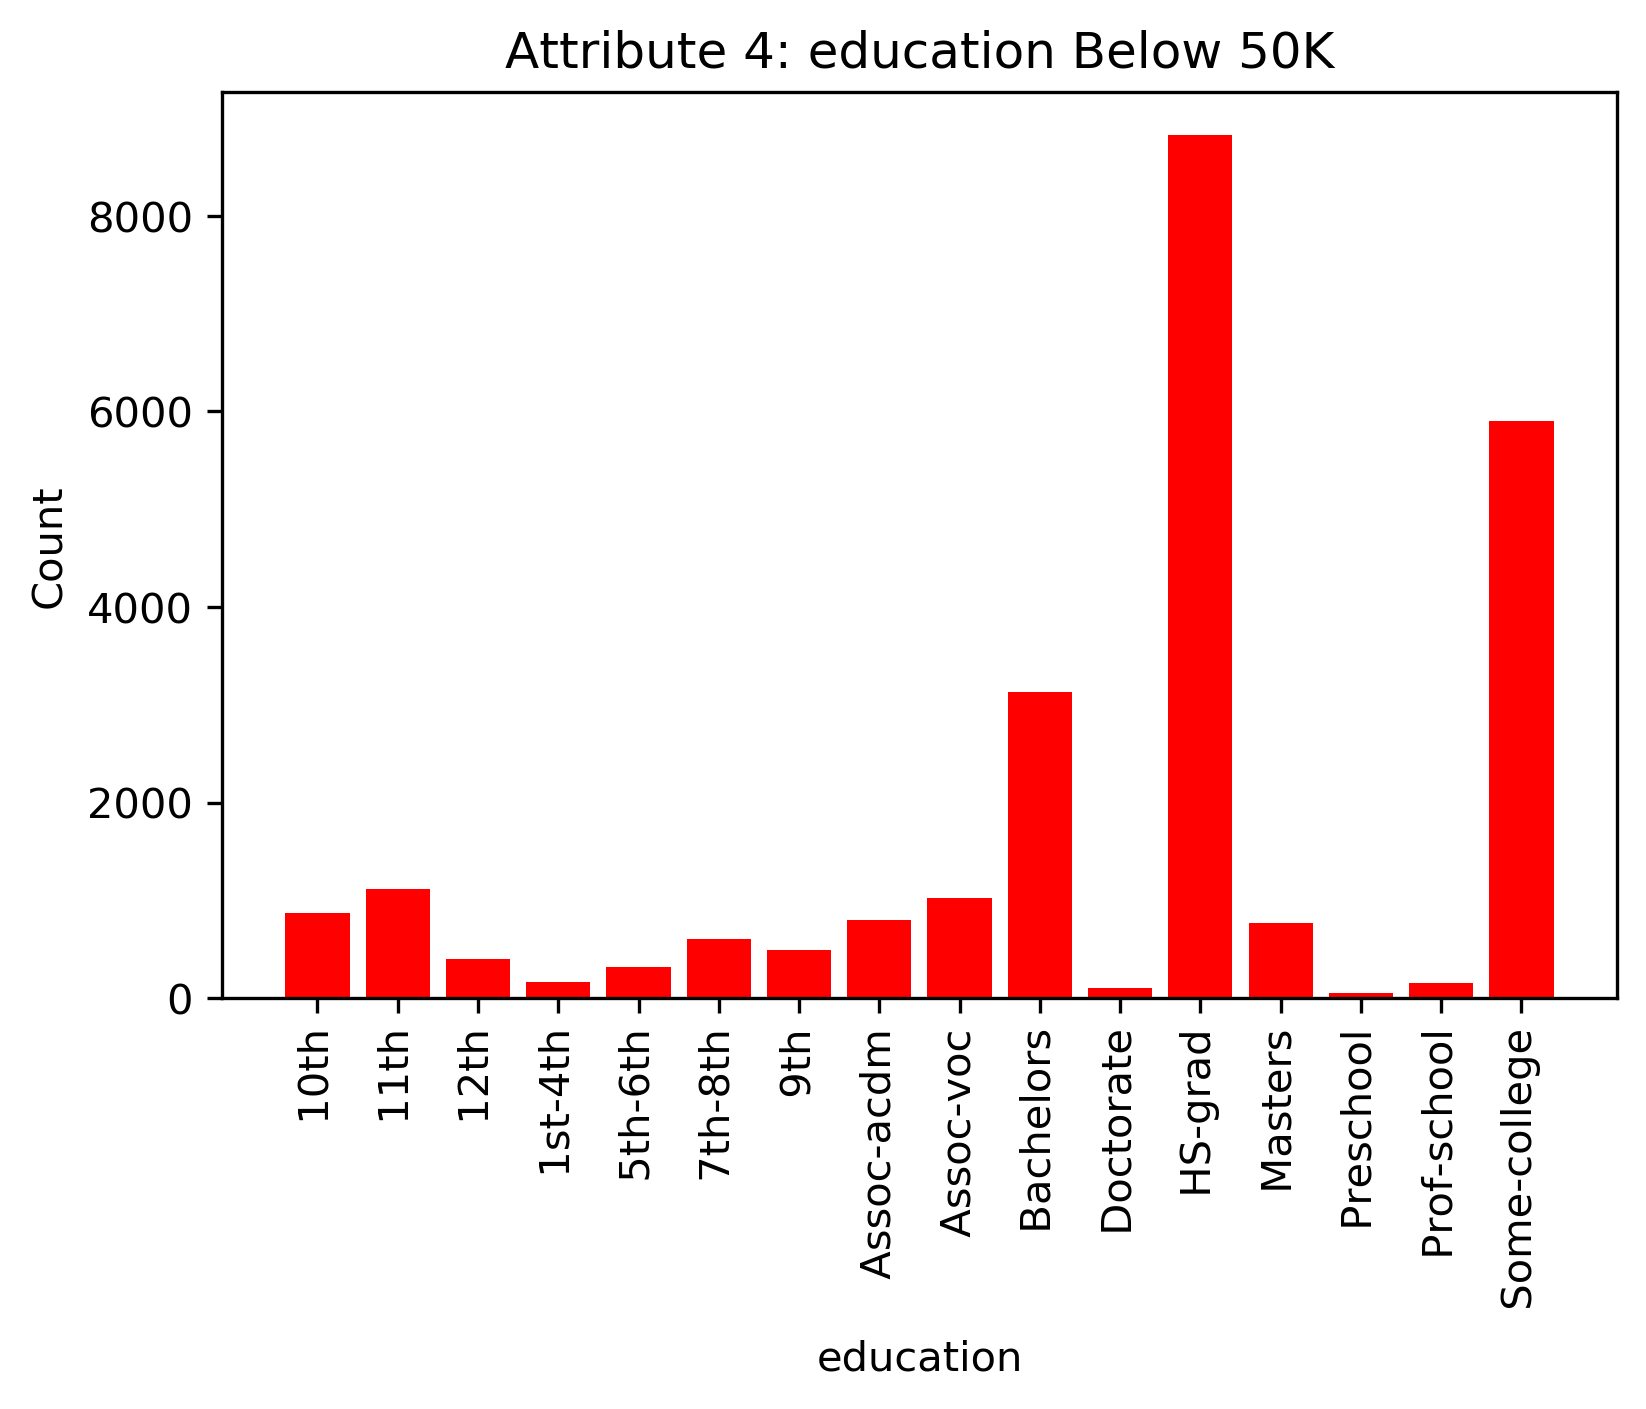
\includegraphics[width=.29\textwidth]{images/3below.png}
			\\~\\
			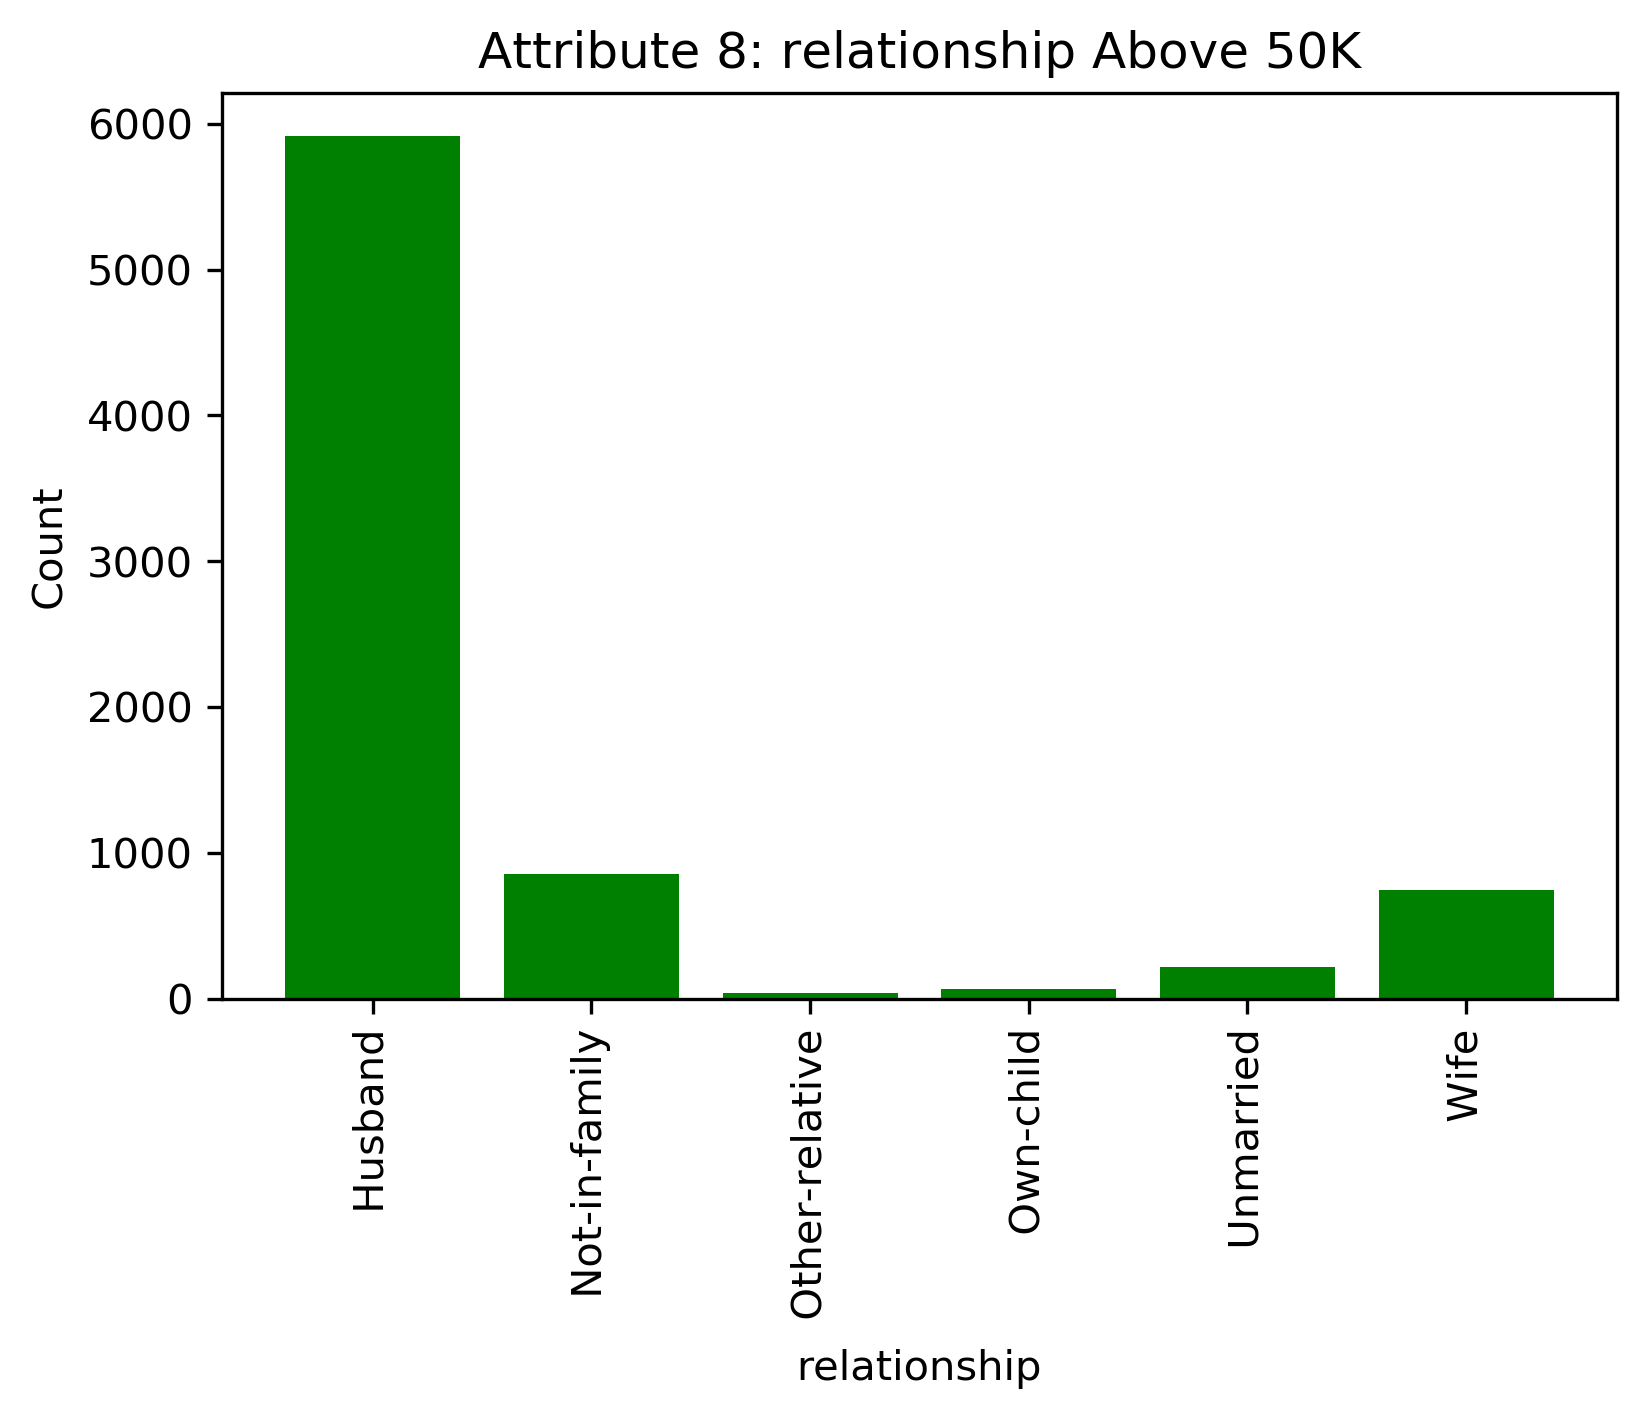
\includegraphics[width=.29\textwidth]{images/7above.png}
			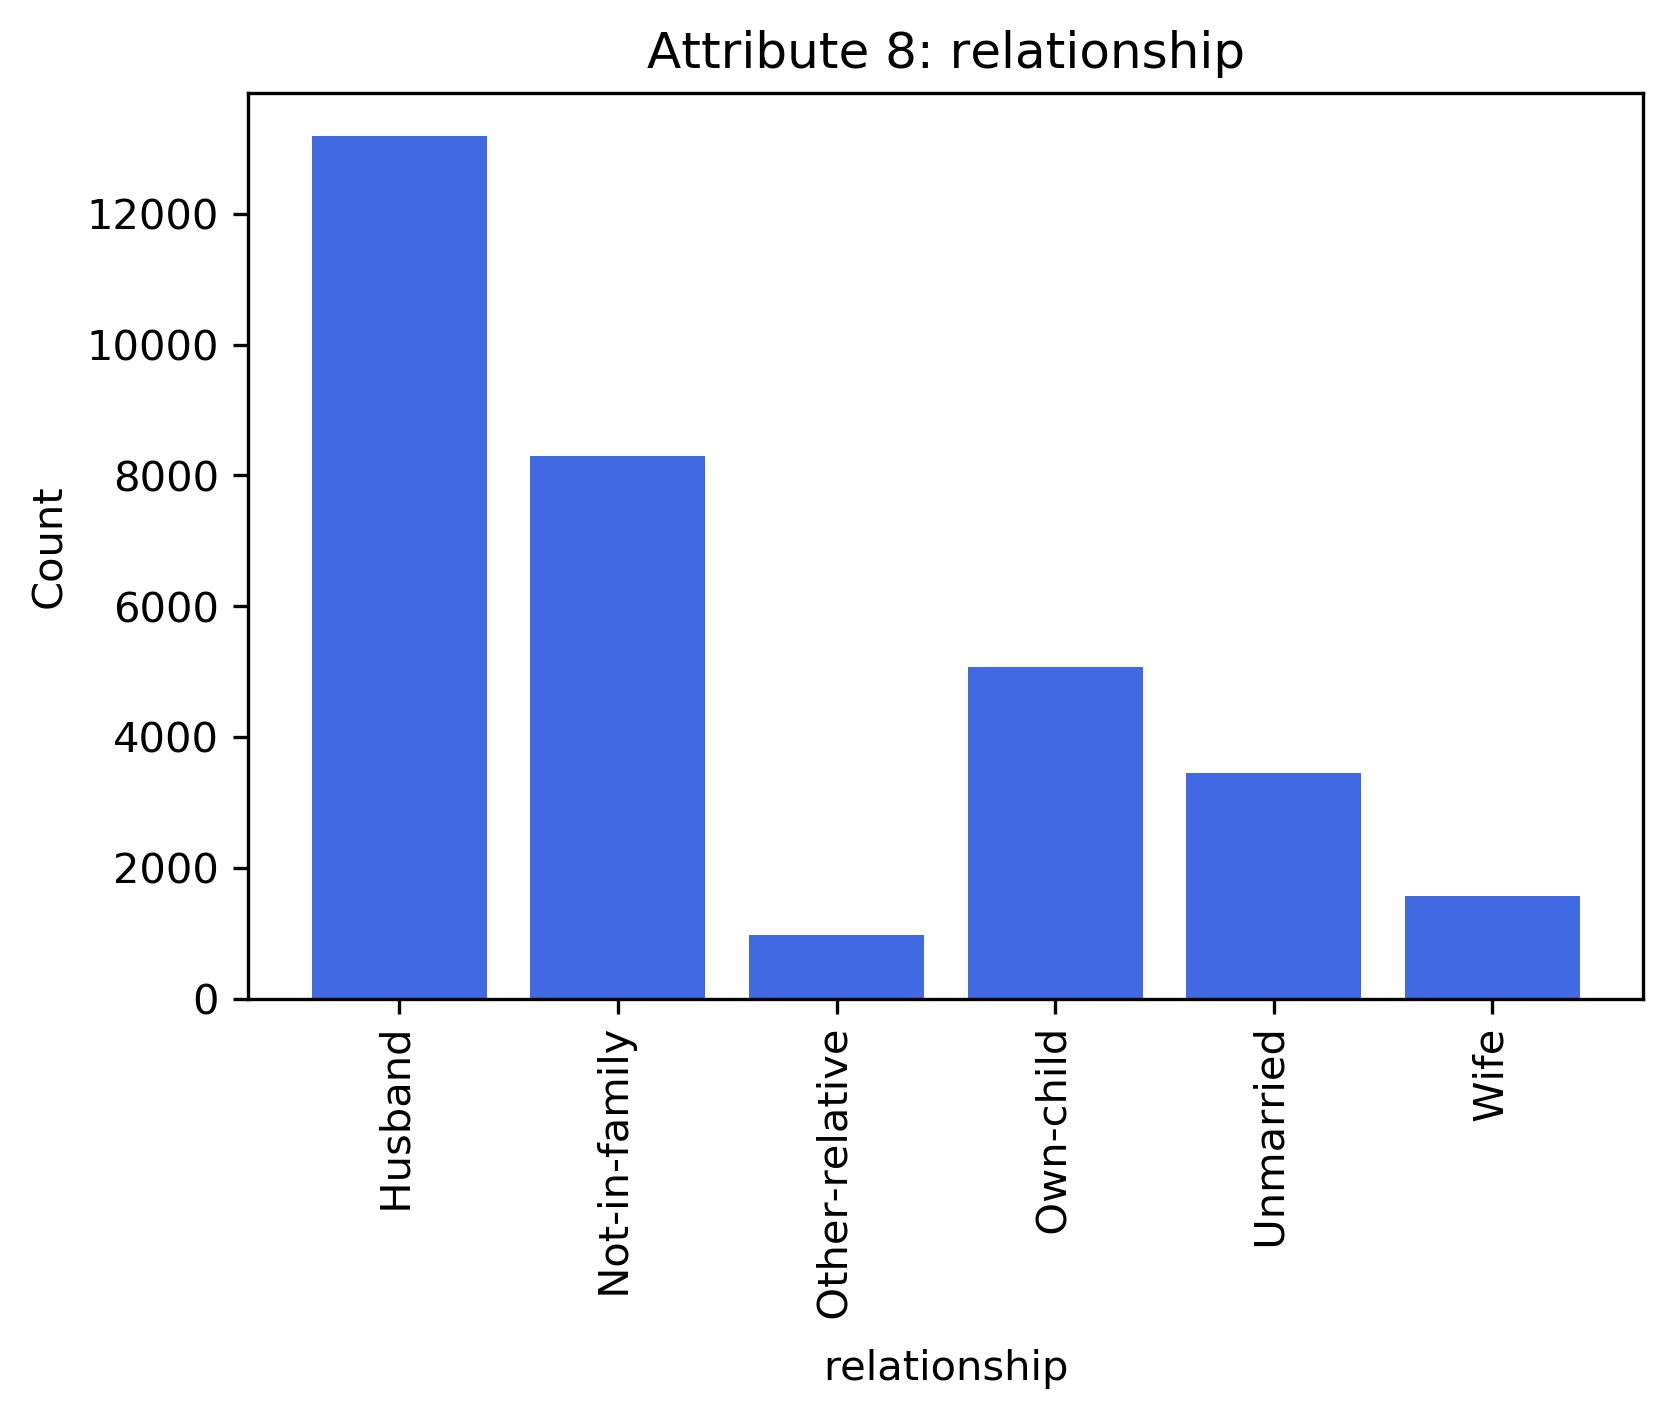
\includegraphics[width=.4\textwidth]{images/7.png}
			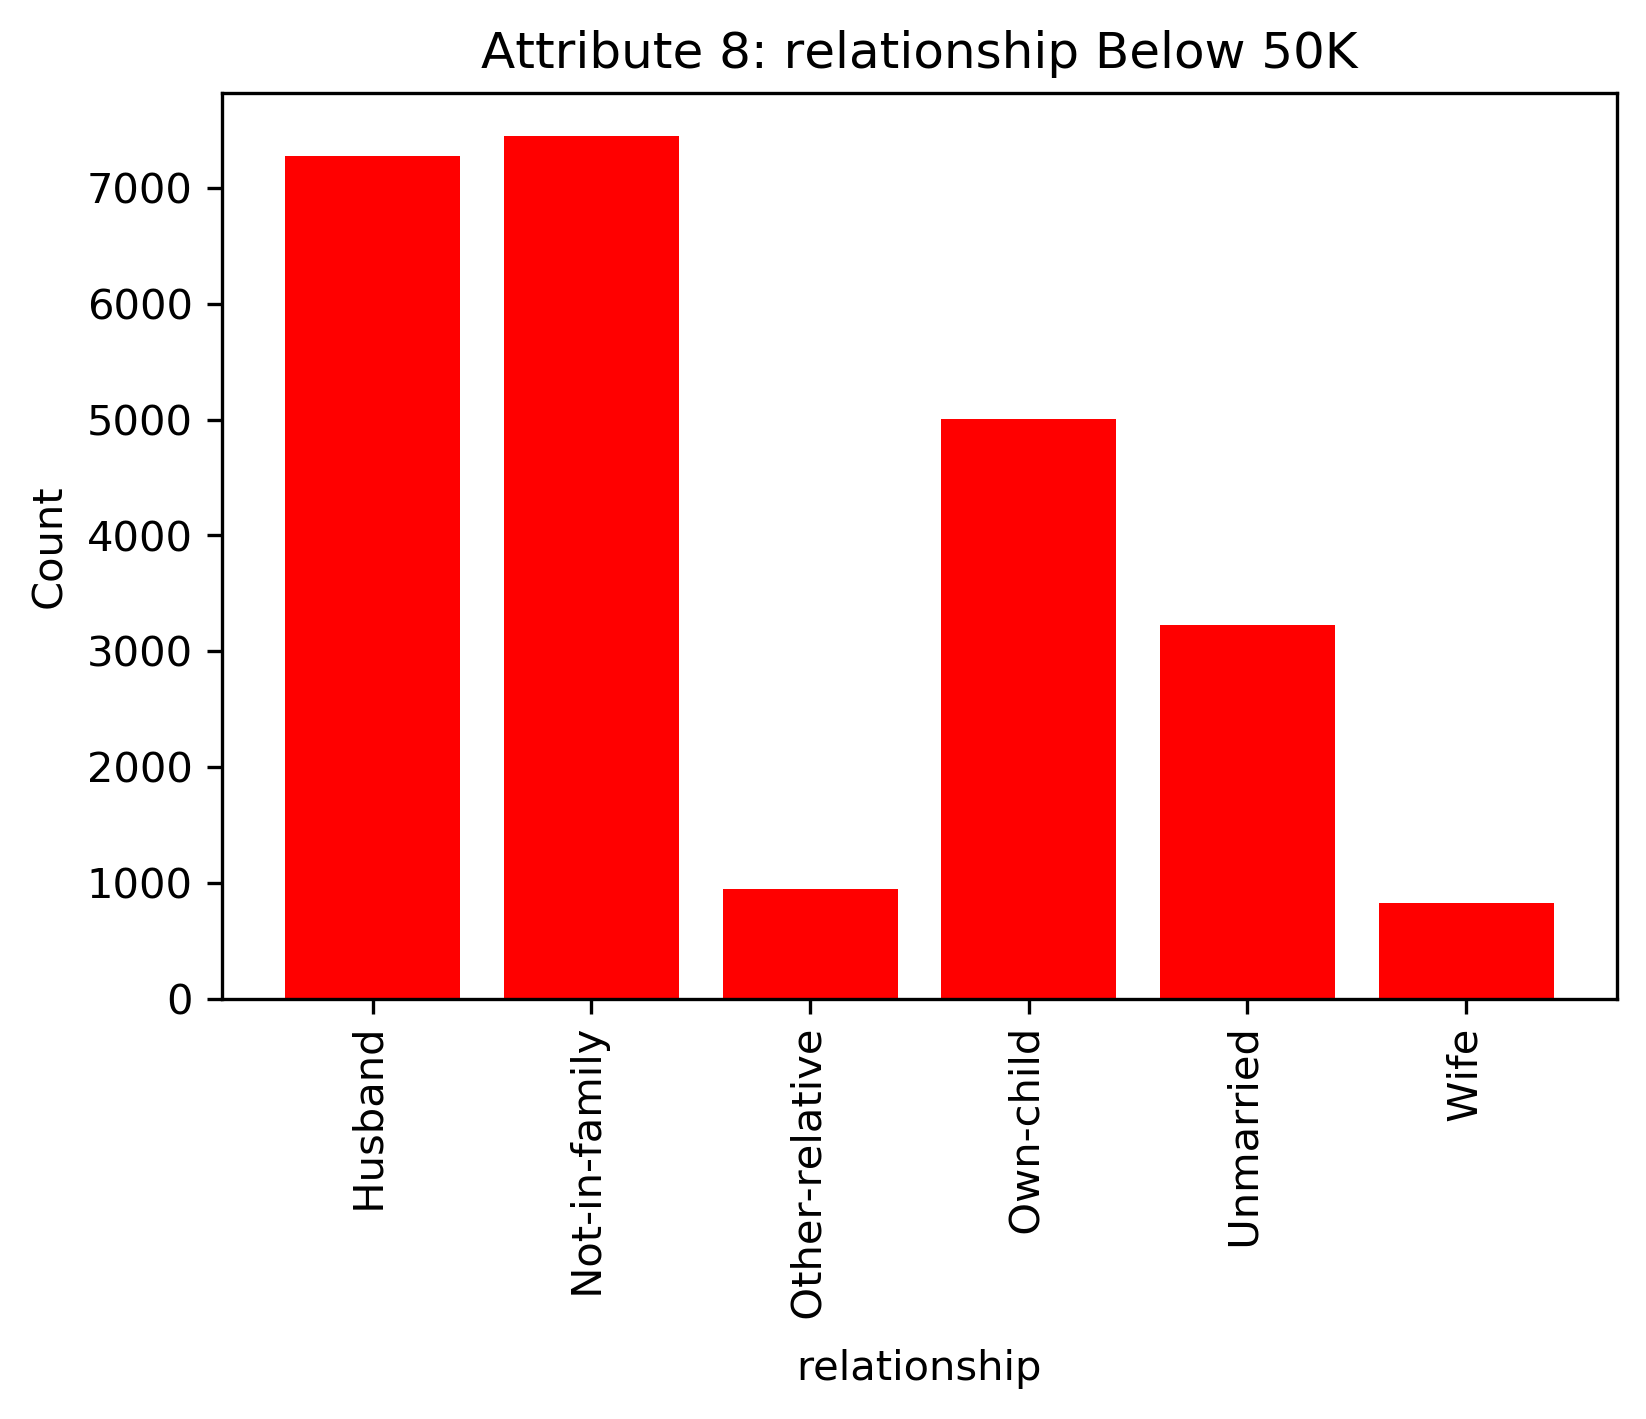
\includegraphics[width=.29\textwidth]{images/7below.png}
			\\~\\
			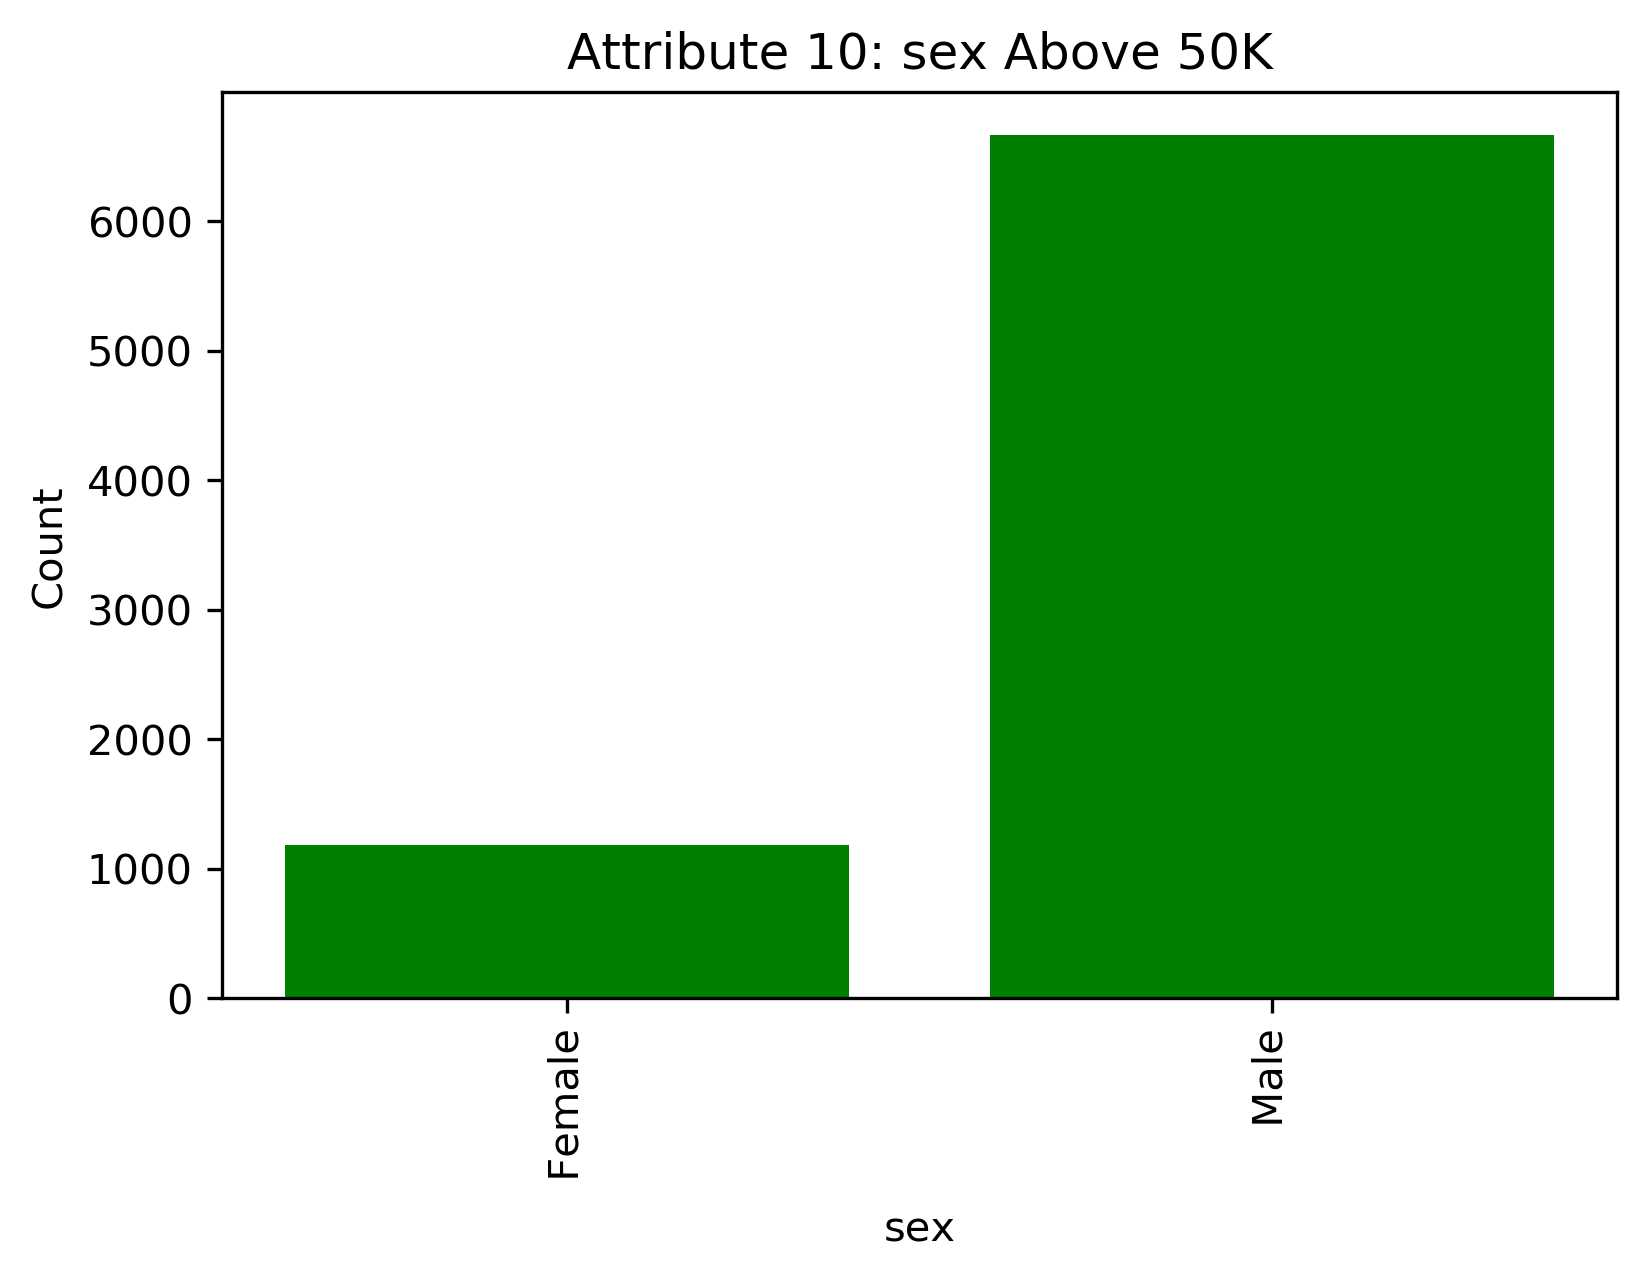
\includegraphics[width=.29\textwidth]{images/9above.png}
			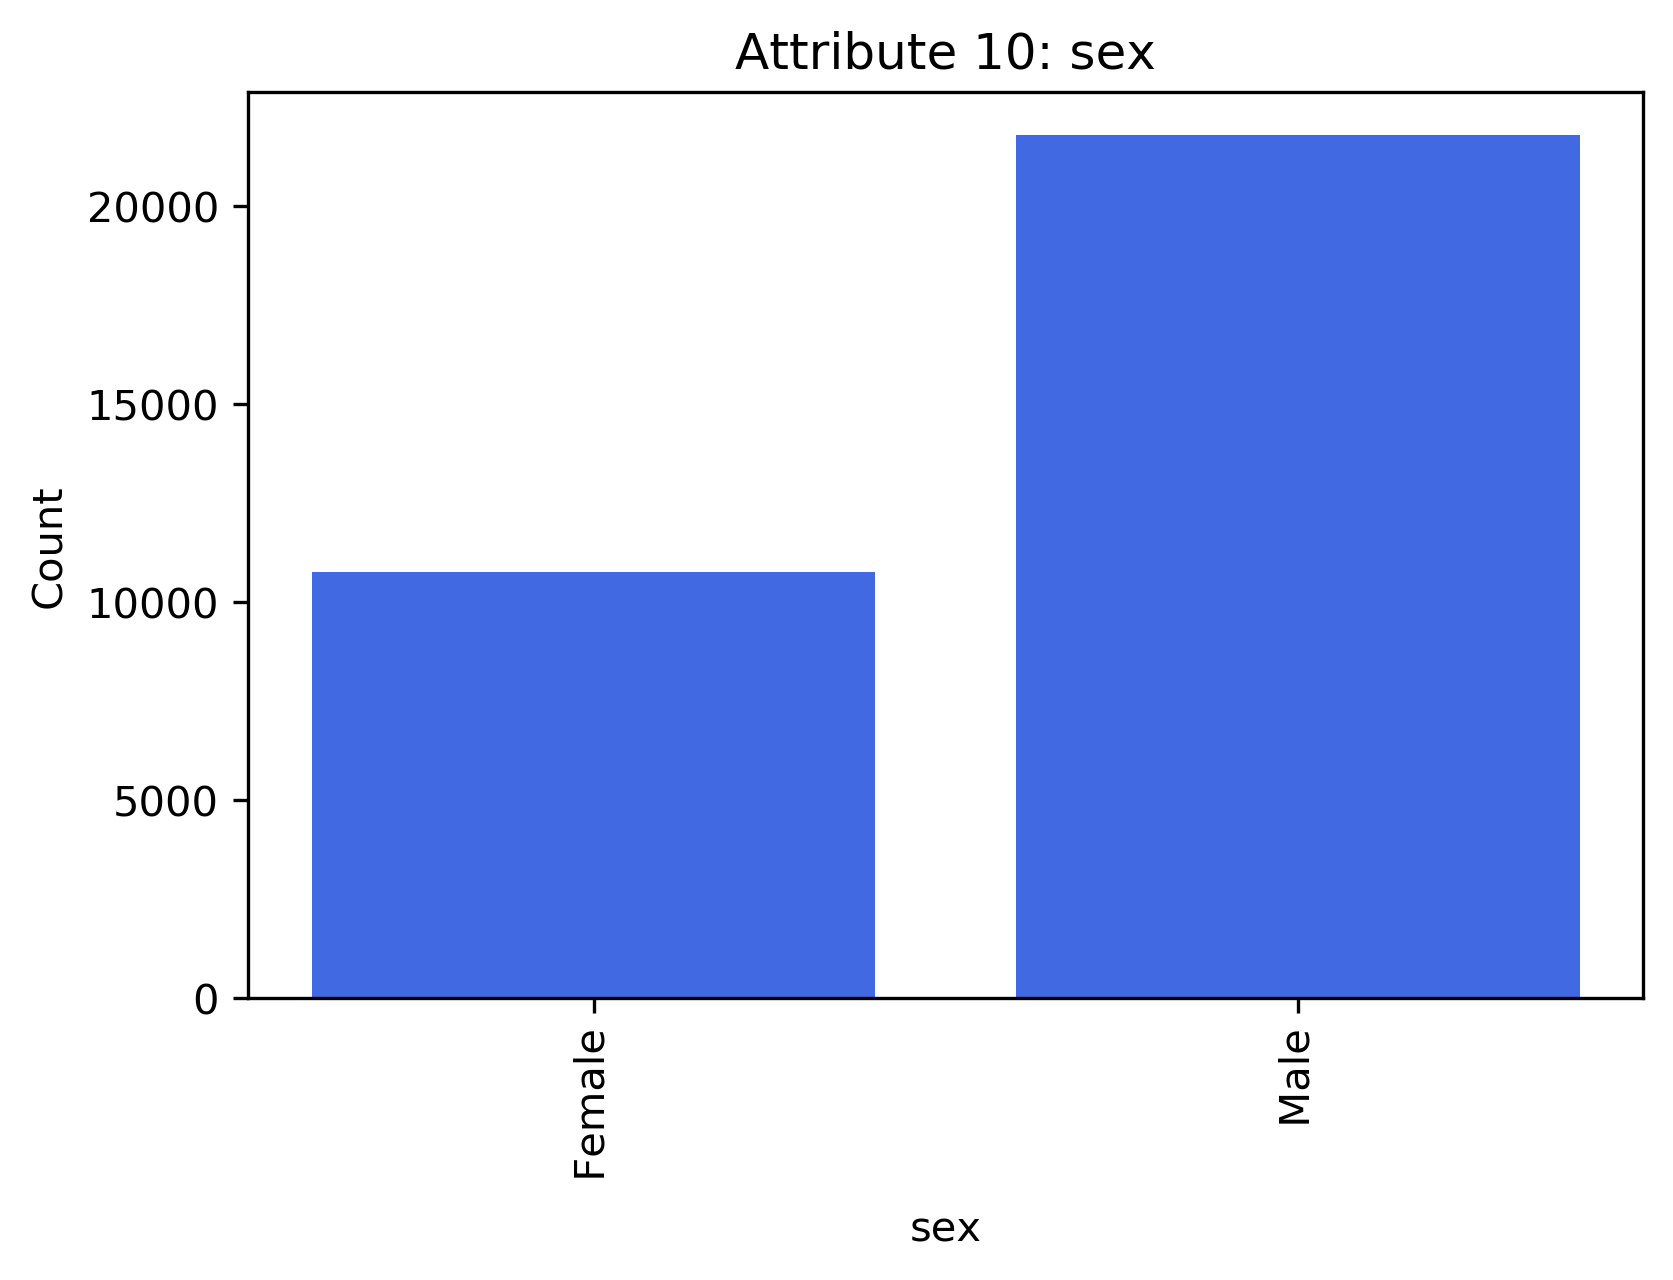
\includegraphics[width=.4\textwidth]{images/9.png}
			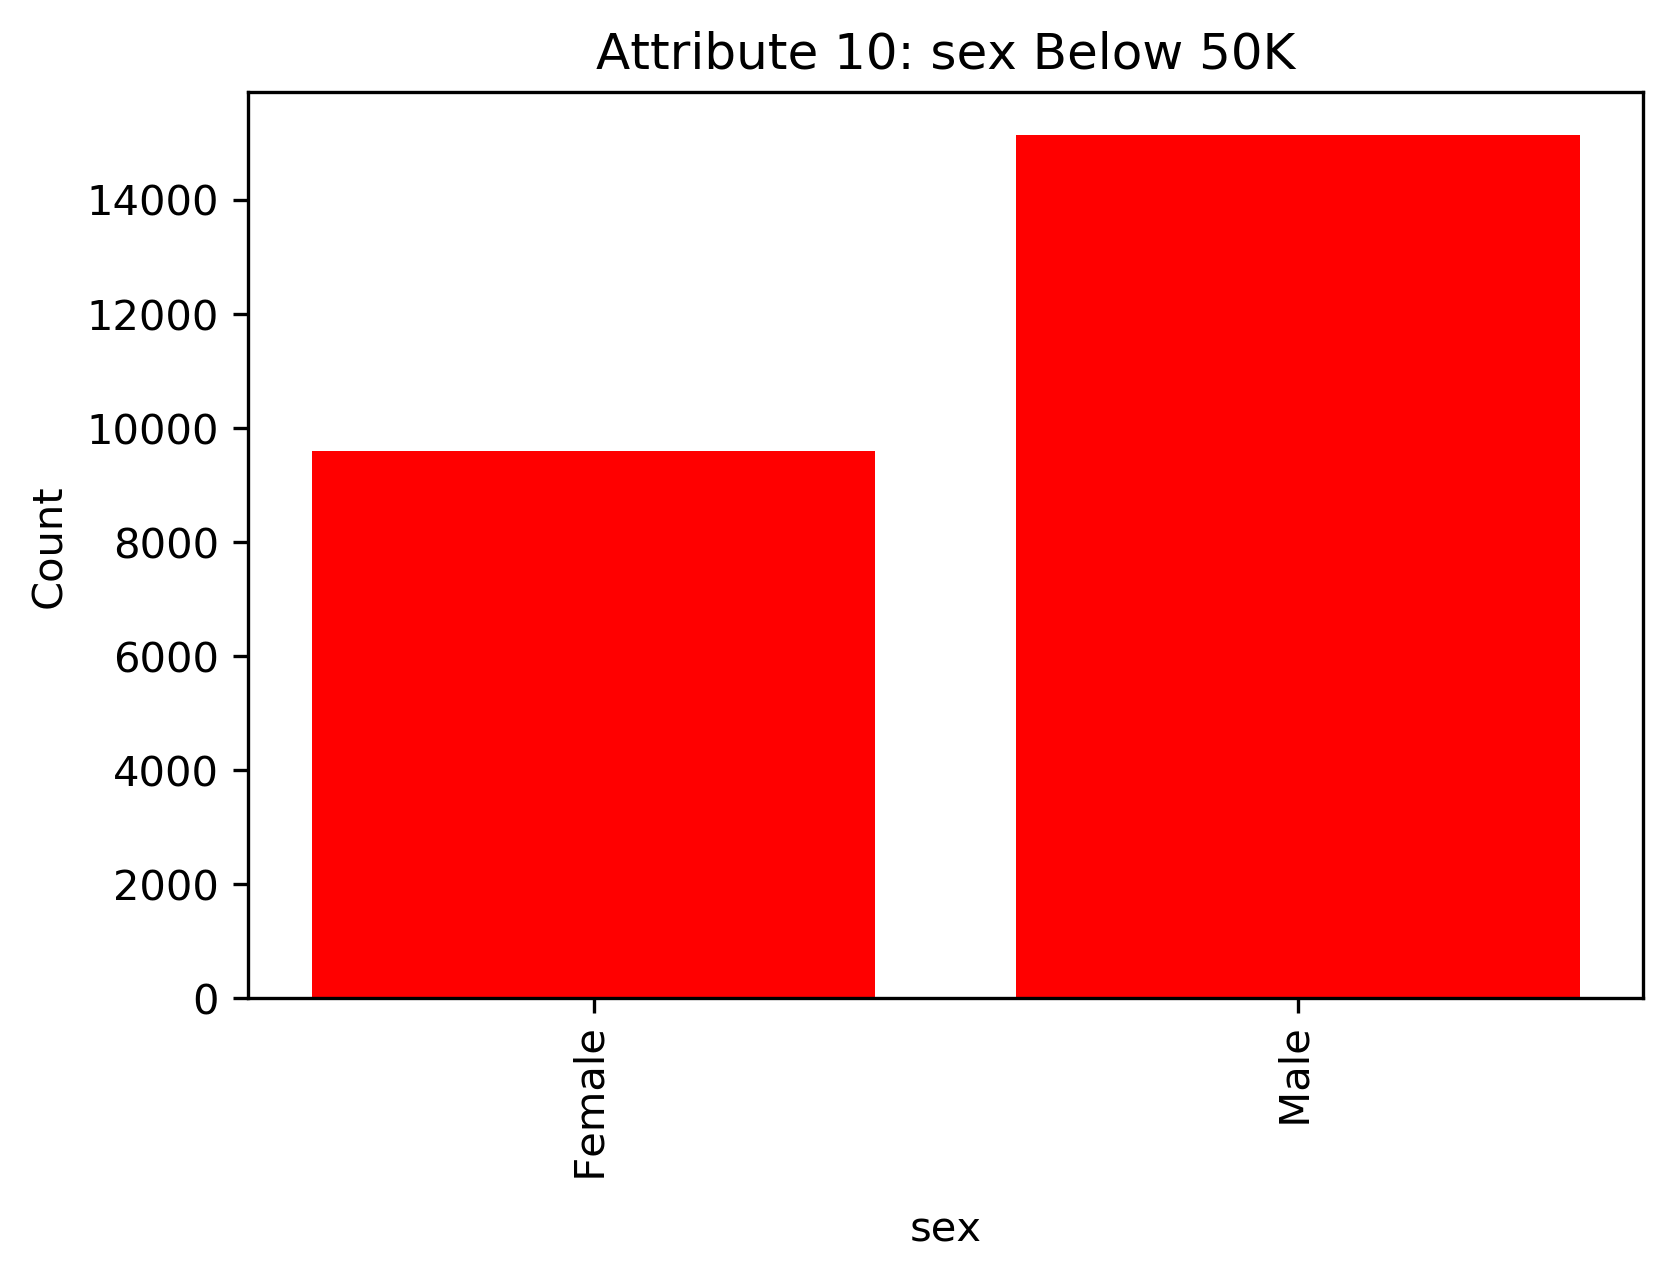
\includegraphics[width=.29\textwidth]{images/9below.png}
			\\~\\
			
		\end{center}
		
		
		\begin{itemize}
			\item 	Benefits: 
			\begin{itemize}
				\item Algorithm will run faster with reduced data
				\item Classifications will not be skewed by unhelpful attributes
				\item Addresses the ``Curse of Dimensionality''
			\end{itemize}
			\item  	Disadvantages: 
			\begin{itemize}
				\item Some information is lost
				\item There is no perfect feature selection technique
			\end{itemize}
		\end{itemize}
		
		
		\subsubsection{Principal Component Analysis}~
		
		This approach maintains the euclidean distance of the standardized data by extracting the $ q $ largest eigen values from the collinearity matrix $ C =\frac{1}{n}X_{norm}X_{norm}^T $. These values are then used with their respective eigen vectors to extract on a smaller set of feature rich data. This method can closely approximate the original, with the $ q $ largest eigen values used. In our case we found that when $ q=5 $ this produced suitable results while still maintaining the integrity of the data.\\
	
	
		
		\begin{itemize}
			\item 	Benefits: 
			\begin{itemize}
				\item Algorithm runs more efficiently on much less information
				\item Addresses the ``Curse of Dimensionality"
			\end{itemize}
			\item  	Disadvantages: 
			\begin{itemize}
				\item Some information is lost
				\item Does not work for linearly dependant data (not invertible).
			\end{itemize}
		\end{itemize}
		
	
	\section{Data Analysis}~
	
	With our four different data processed formats we can begin to fit these sets to different data classifying techniques. We have chosen a collection of methods, based on both supervised and unsupervised algorithms. We have emphasised our analysis on supervised techniques. With specific details on each method's approach and results.
	

	
		\subsection{Naive Bayes}~
		
		This technique is based on Bayes theorem to determine whether or not a person is in the class making more or less than $ 50 000USD$ a year. This is based on what is known to be true from the training set. It allows us to establish a class based on the occurrences of the 30000 people trained on. 
		
		\begin{equation}
		P(c|a_1,a_2,...,a_j) = \dfrac{P(a_1|c)...P(a_j|c)P(c)}{P(a_1,a_2,...,a_j)}
		\end{equation}
		$ c= $ Class, $ a_i = i^{th}$ Attribute\\
		
		
		The more attributes we add with a large dataset will further refine these results. Running this model on our four data sets results in the following confusion matrices:
	
		\begin{center}
			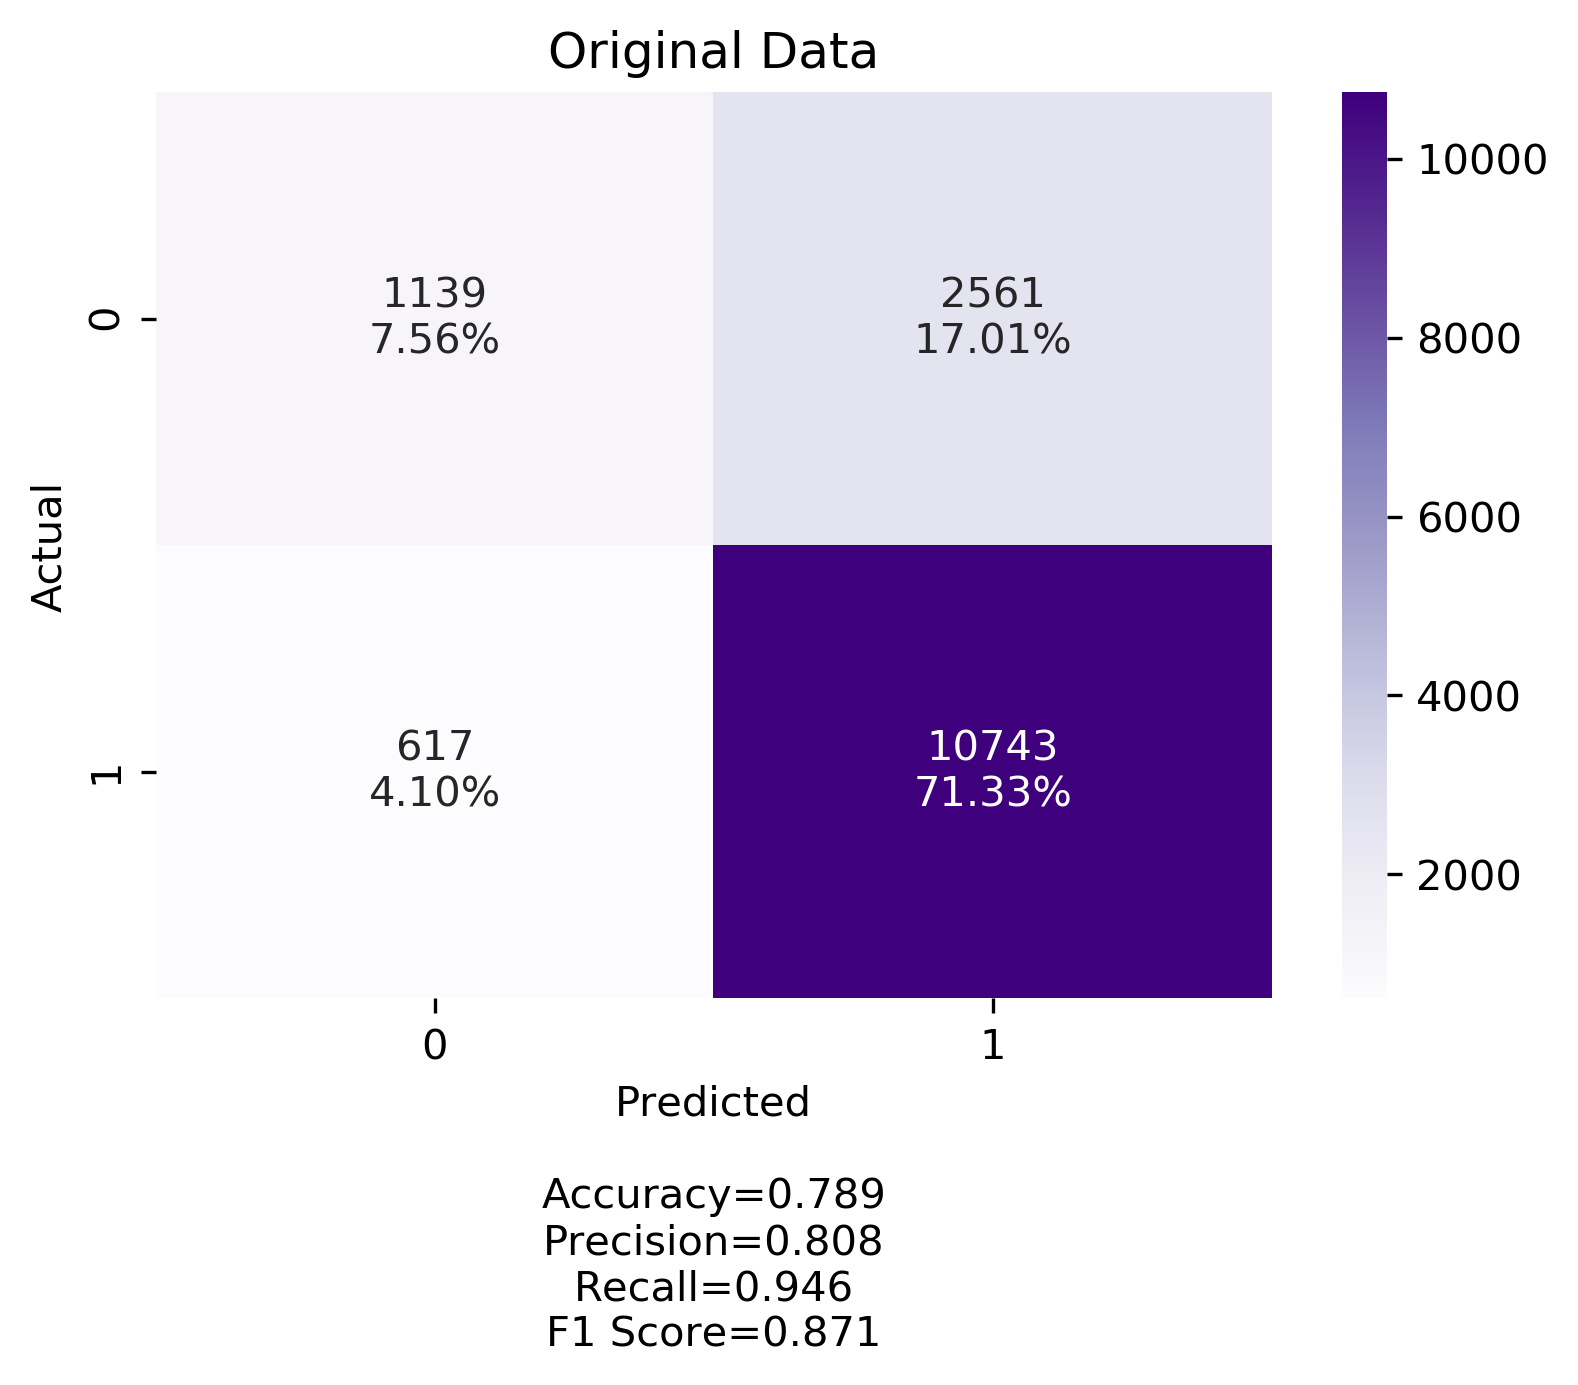
\includegraphics[width=.45\textwidth]{images/cf1.png}
			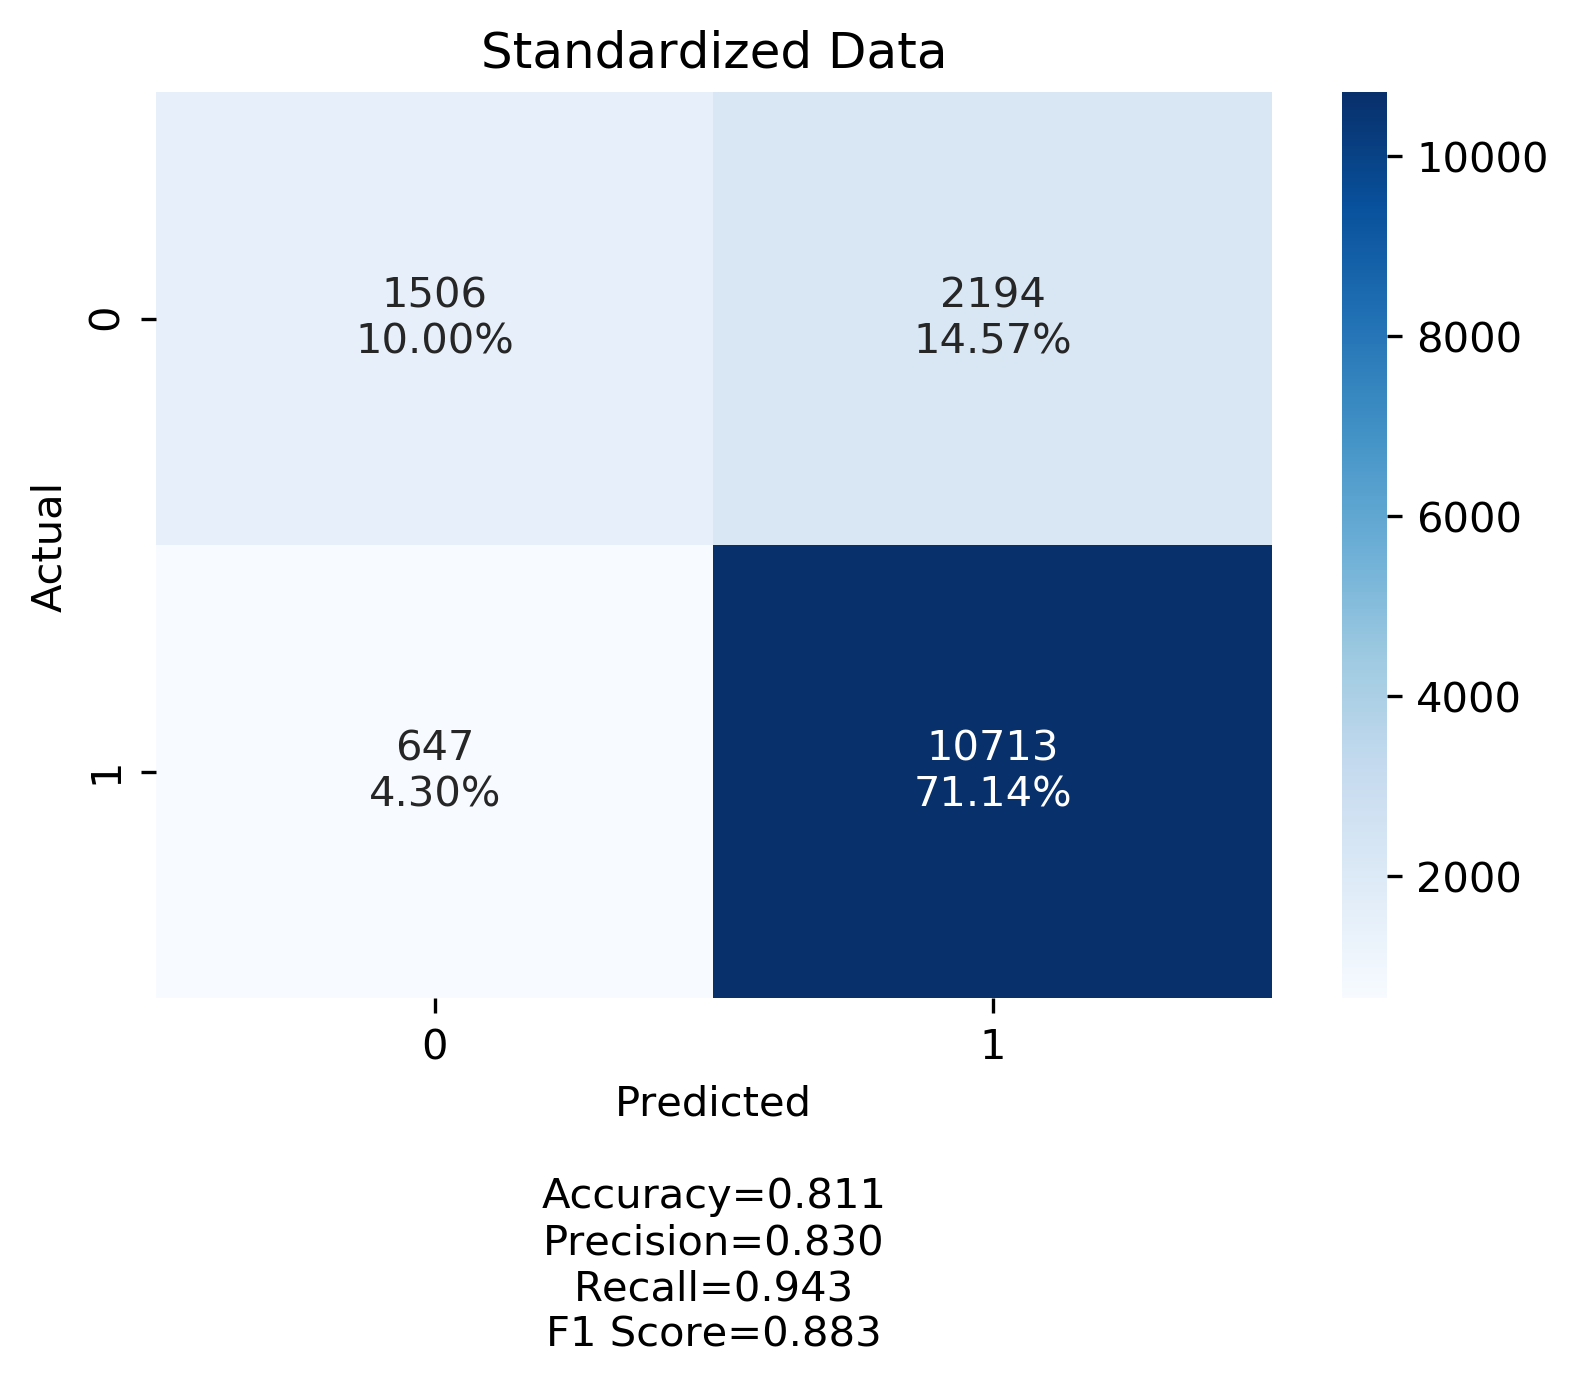
\includegraphics[width=.45\textwidth]{images/cf2.png}
			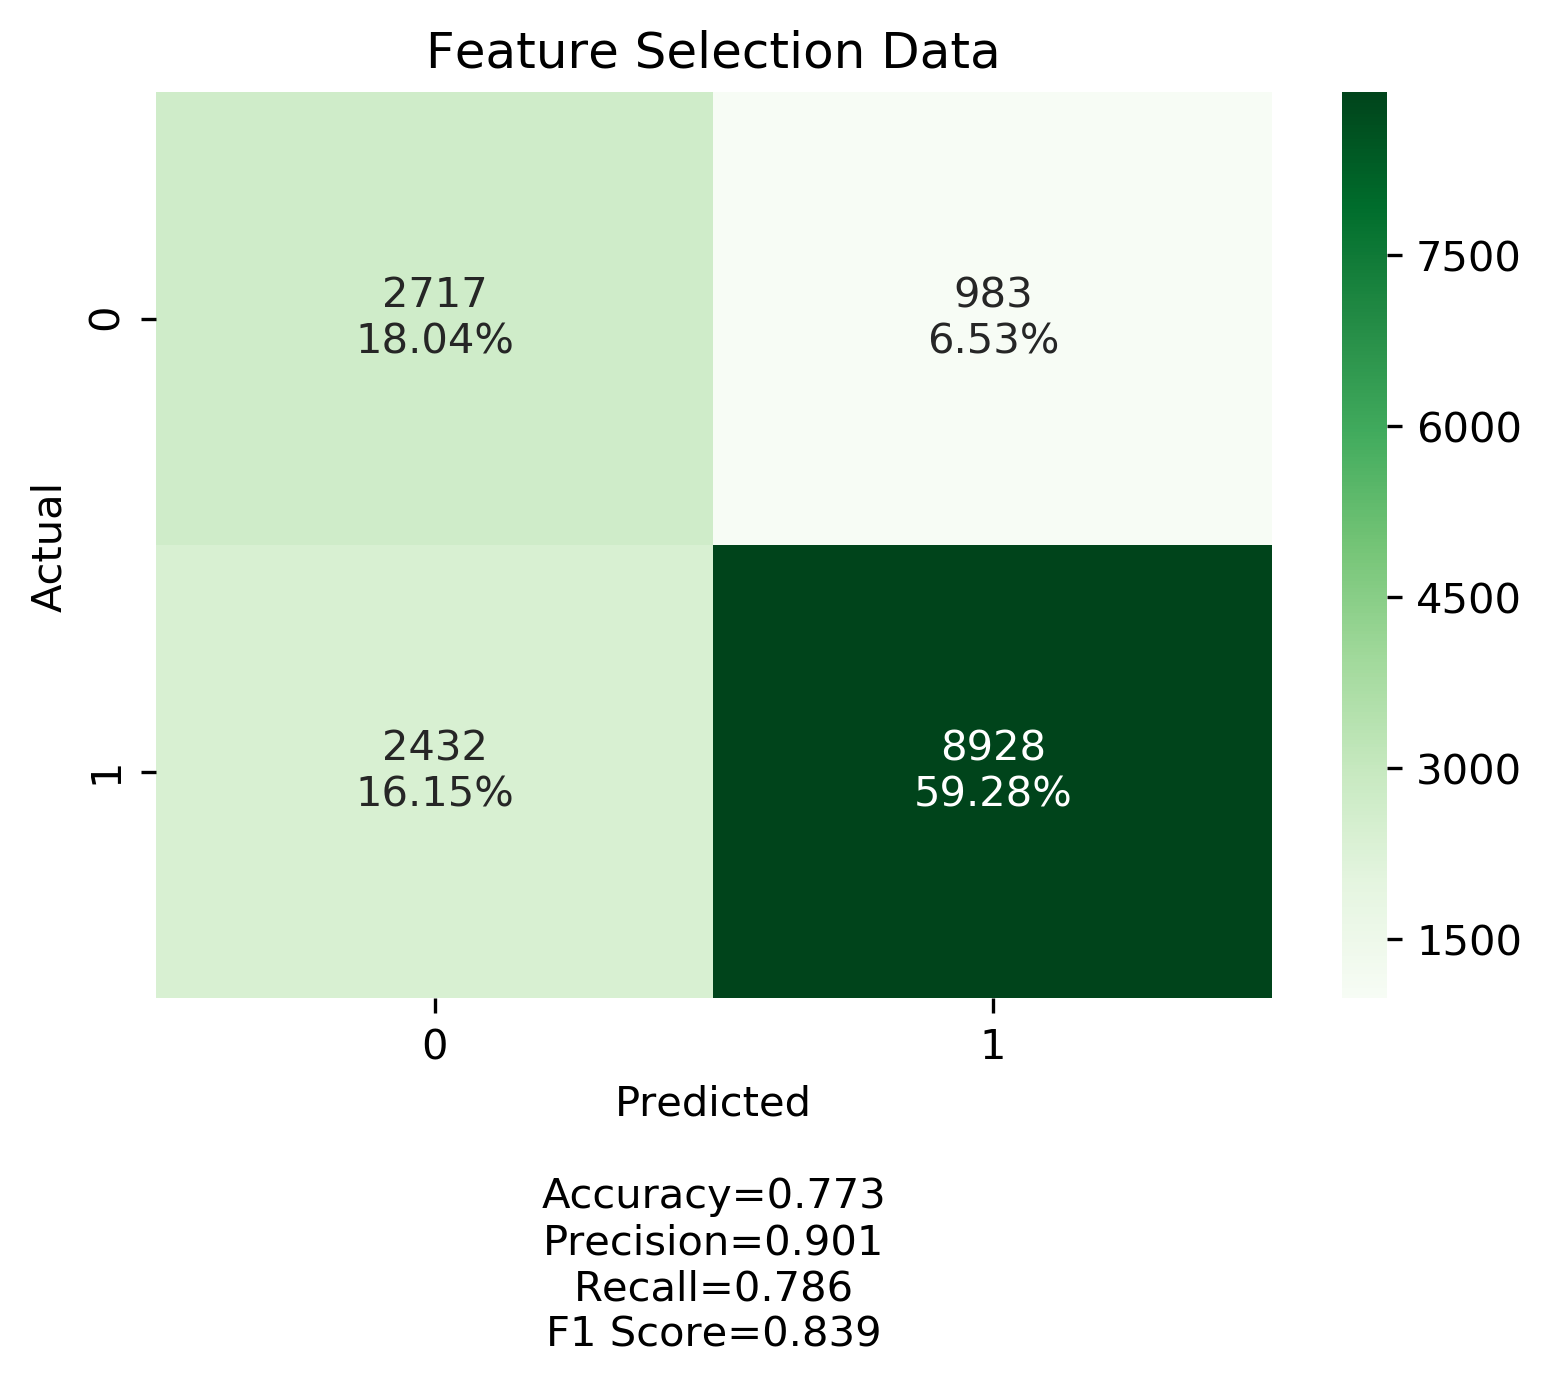
\includegraphics[width=.45\textwidth]{images/cf3.png}
			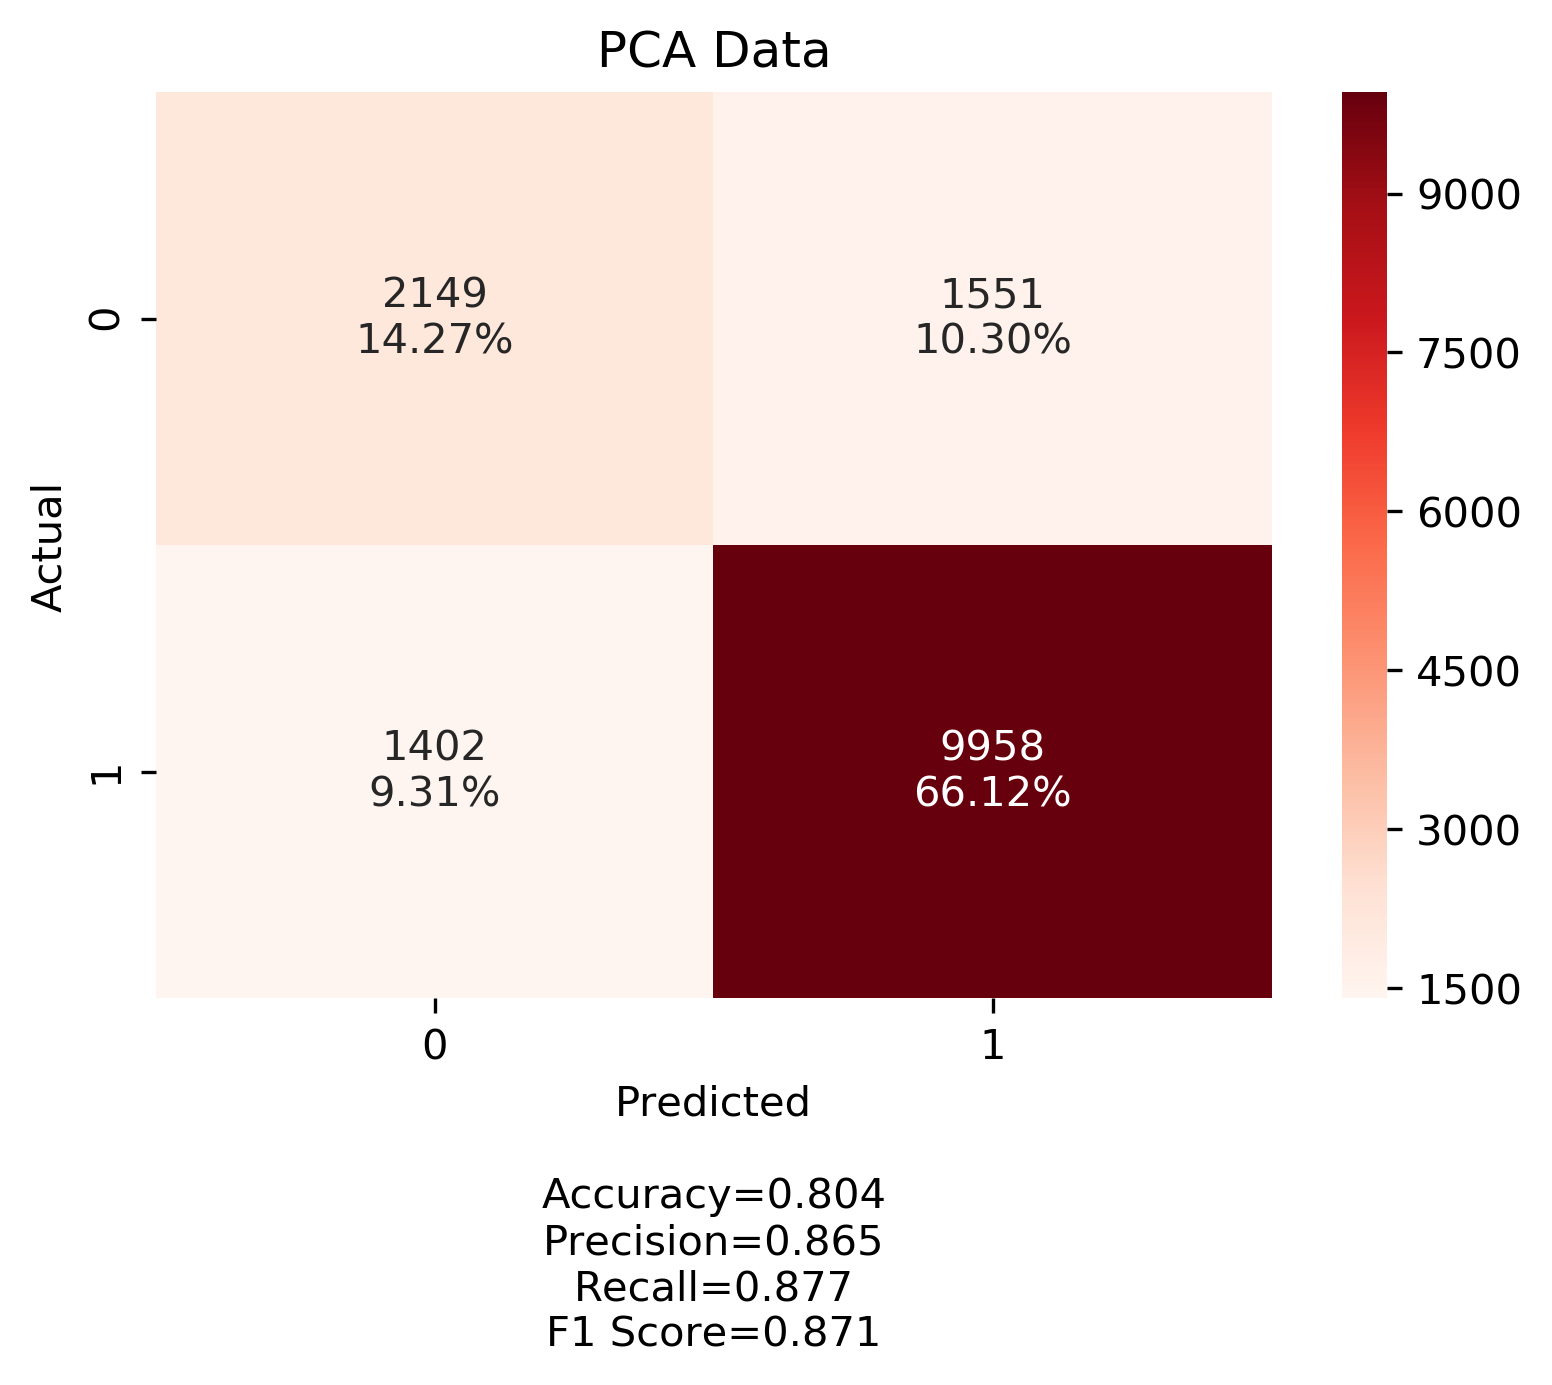
\includegraphics[width=.45\textwidth]{images/cf4.png}		
		\end{center}
		
		
		Things to Consider:
		\begin{itemize}
			\item This approach does not do well with unknown data as this will cause a greater weight to be assumed on all other attributes.
			\item The mathematics of Bayes in this model assumes all attributes are completely independent. The accuracy of this prediction is affected if this is not true.\\
		\end{itemize}
		
		
		\subsection{Logistical Regression}~
		
		The idea behind logistical regression is similar to the perception algorithm. The difference being an added confidence measure for how good our prediction is once we establish some line that splits the data across classes. The distance of a single point from this line will then produce a probability of accuracy for the class prediction.
		
		\begin{equation}
		S(\mathbf{w}^T\mathbf{x}) = \dfrac{1}{1+e^{-\mathbf{w}^T\mathbf{x}}}
		\end{equation}
		$ \mathbf{w} = $ found linear separator\\ 
		
		The $ \mathbf{w} $ vector can be found a few different ways using linear algebra on an independent matrix, or approximated using a gradient descent algorithm. We have implemented the model fit with \emph{sklearn}, and are abstracted from this tuning parameter. Running this model on our four data sets results in the following confusion matrices:
		
		\begin{center}
			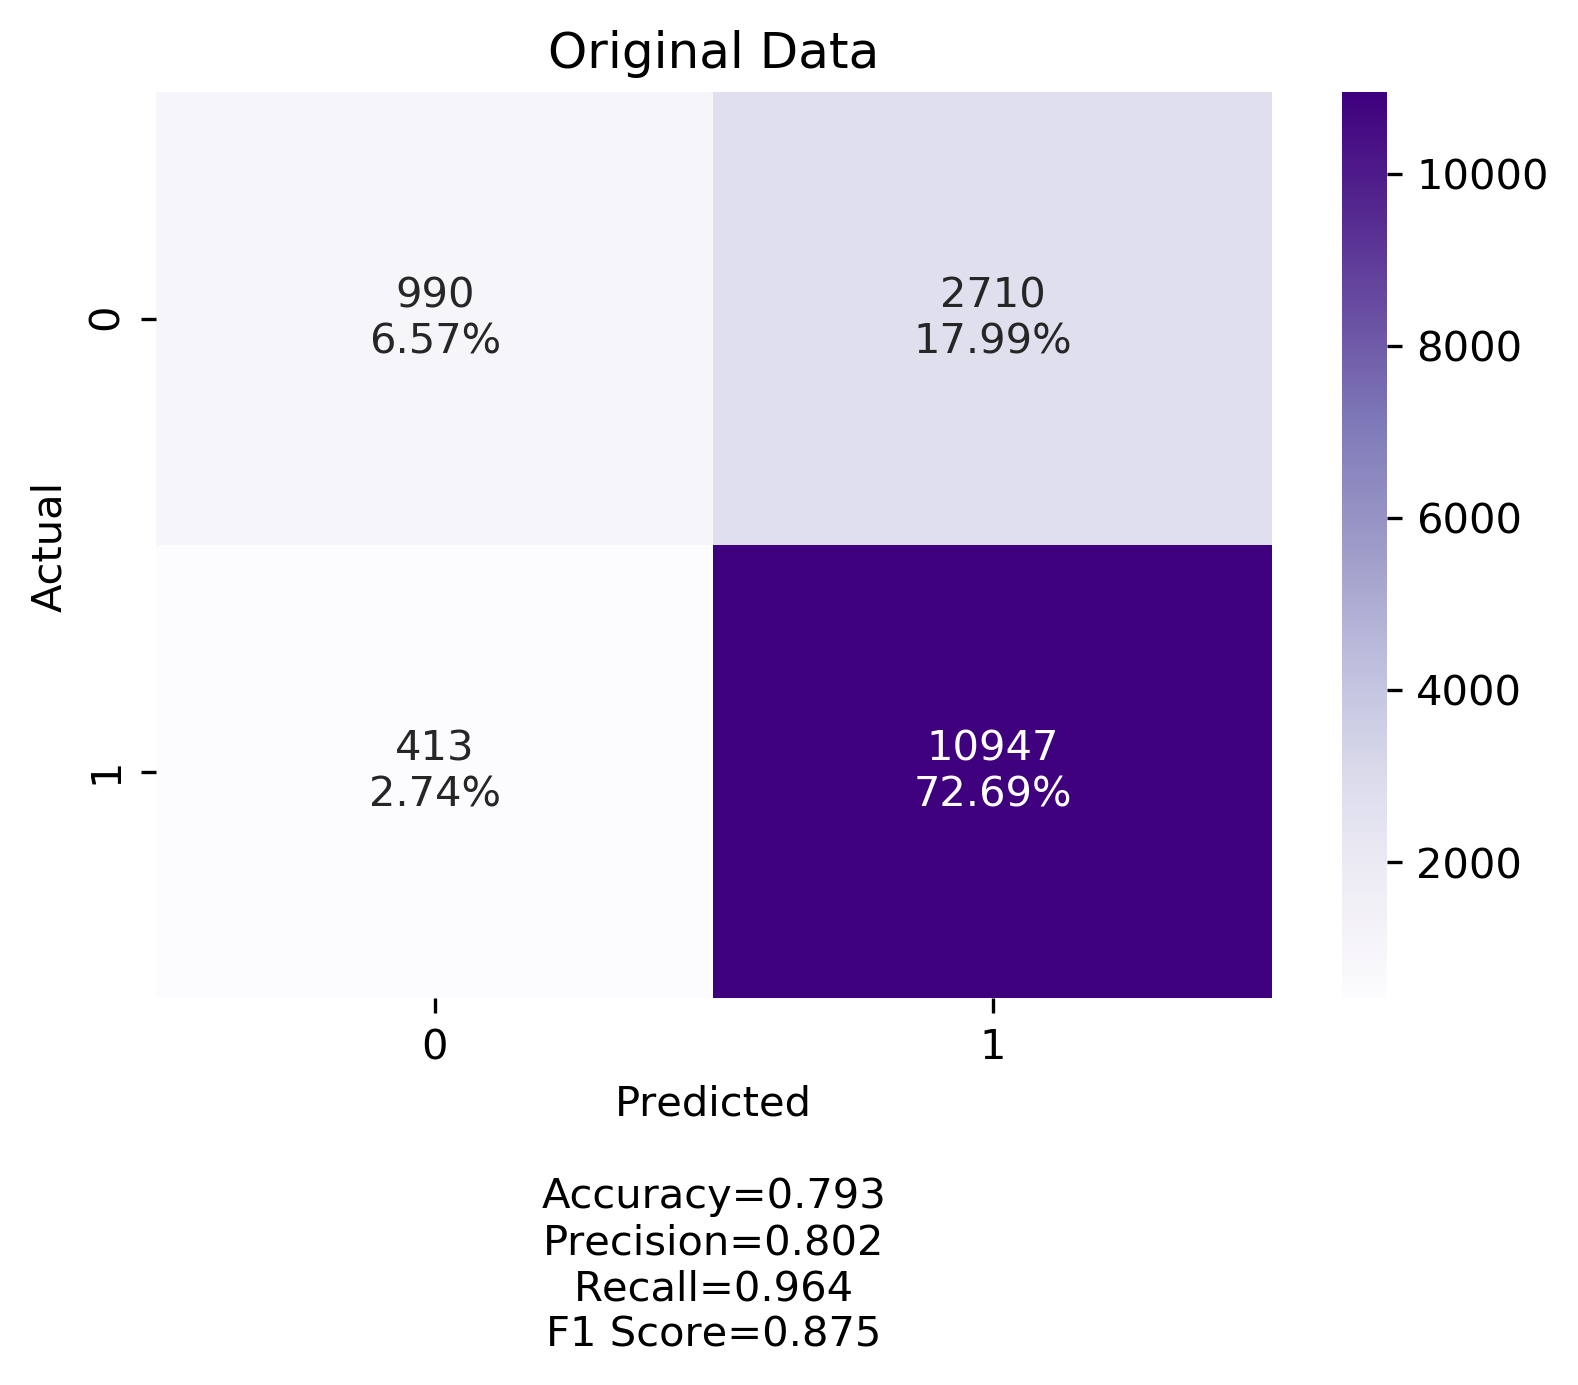
\includegraphics[width=.45\textwidth]{images/cf5.png}
			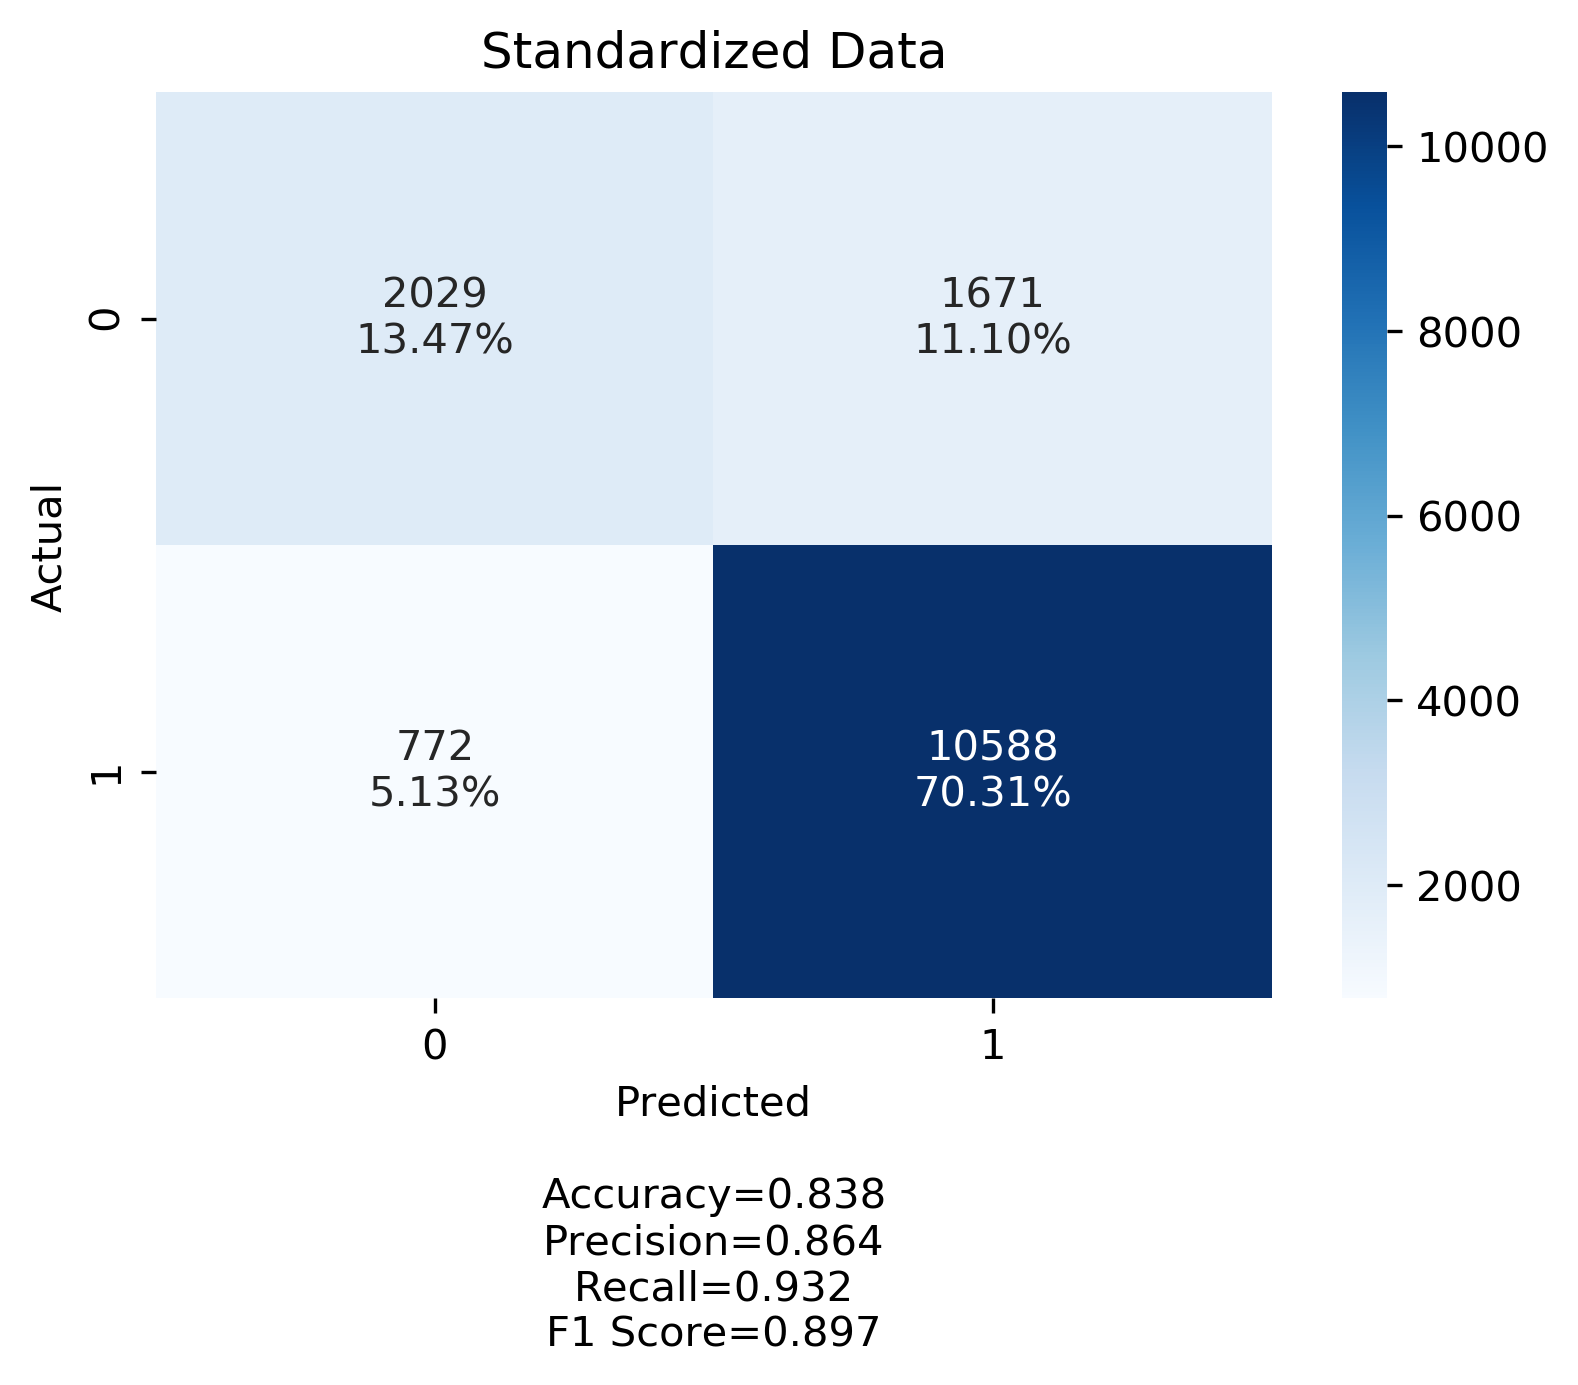
\includegraphics[width=.45\textwidth]{images/cf6.png}
			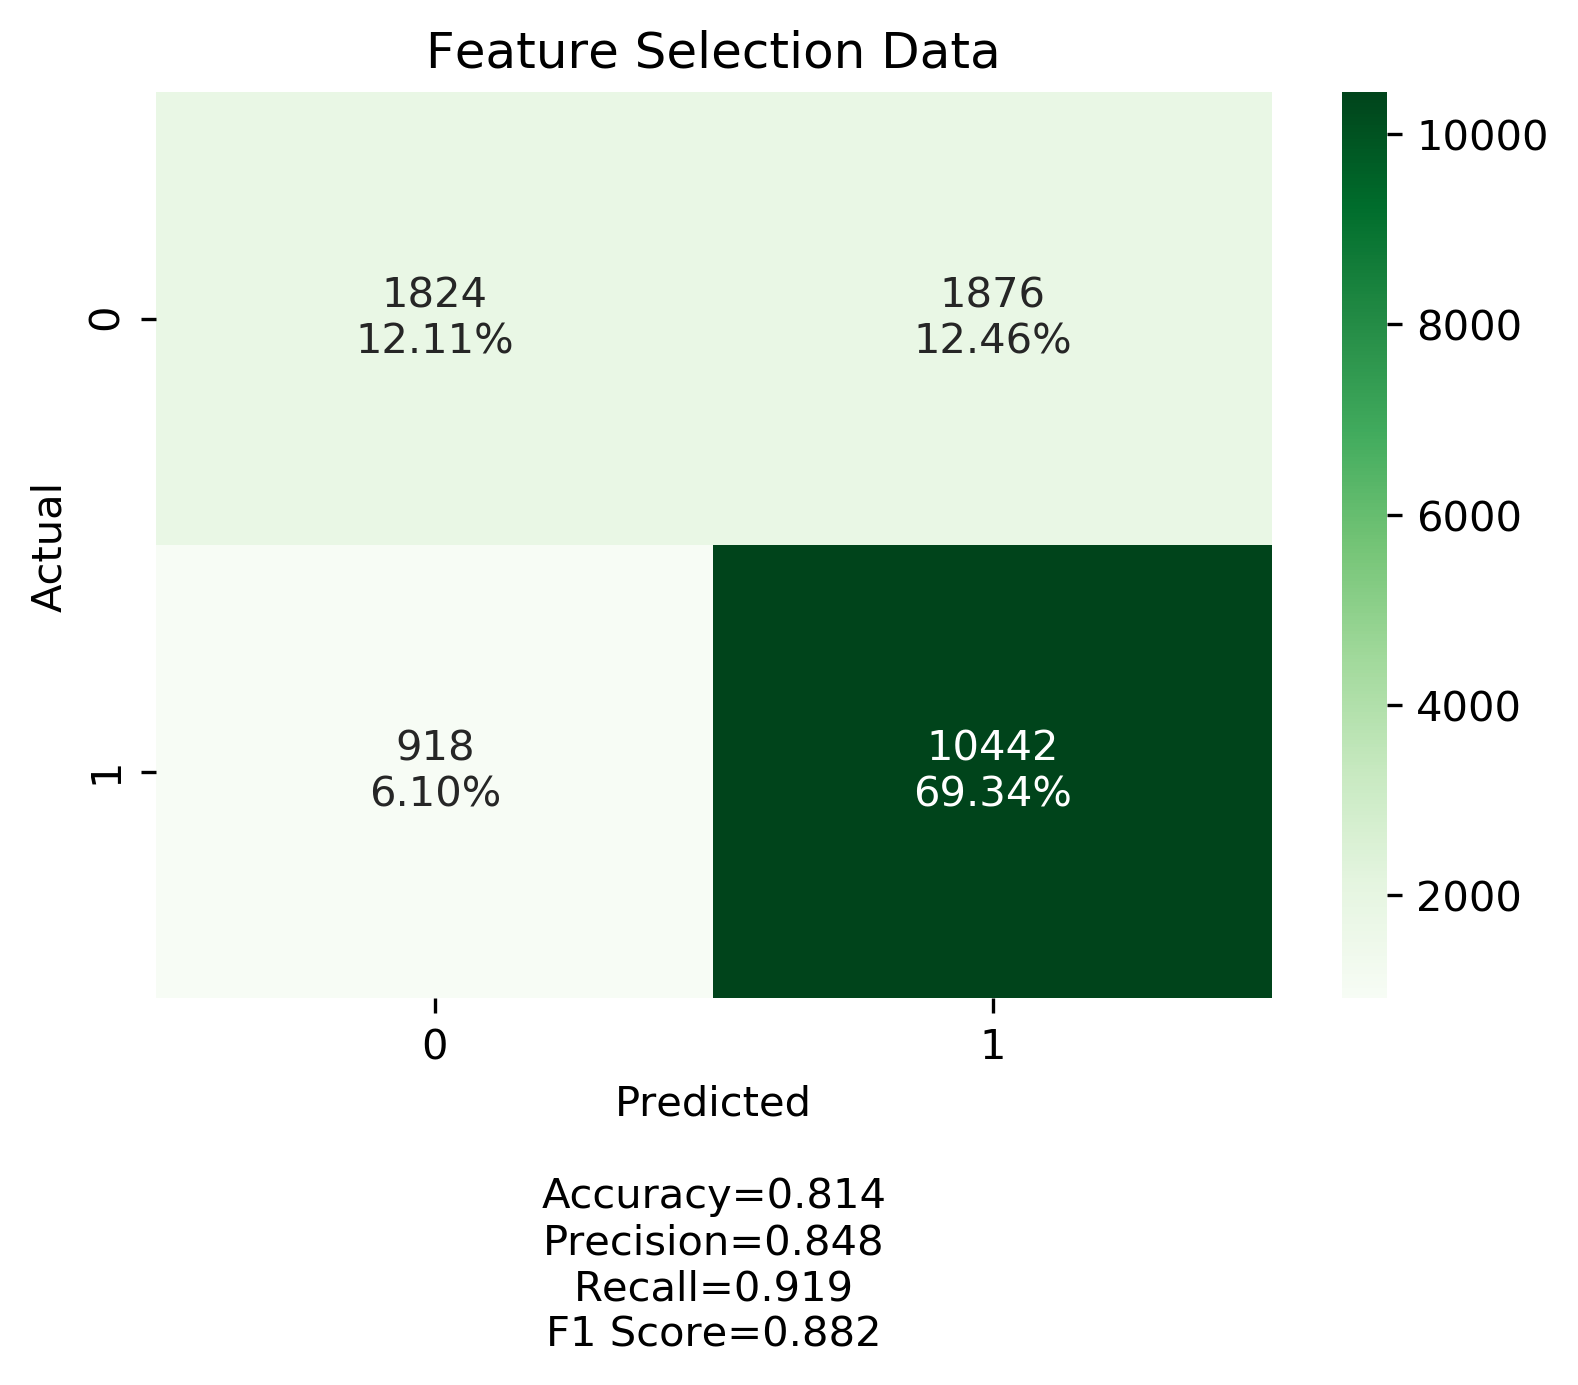
\includegraphics[width=.45\textwidth]{images/cf7.png}
			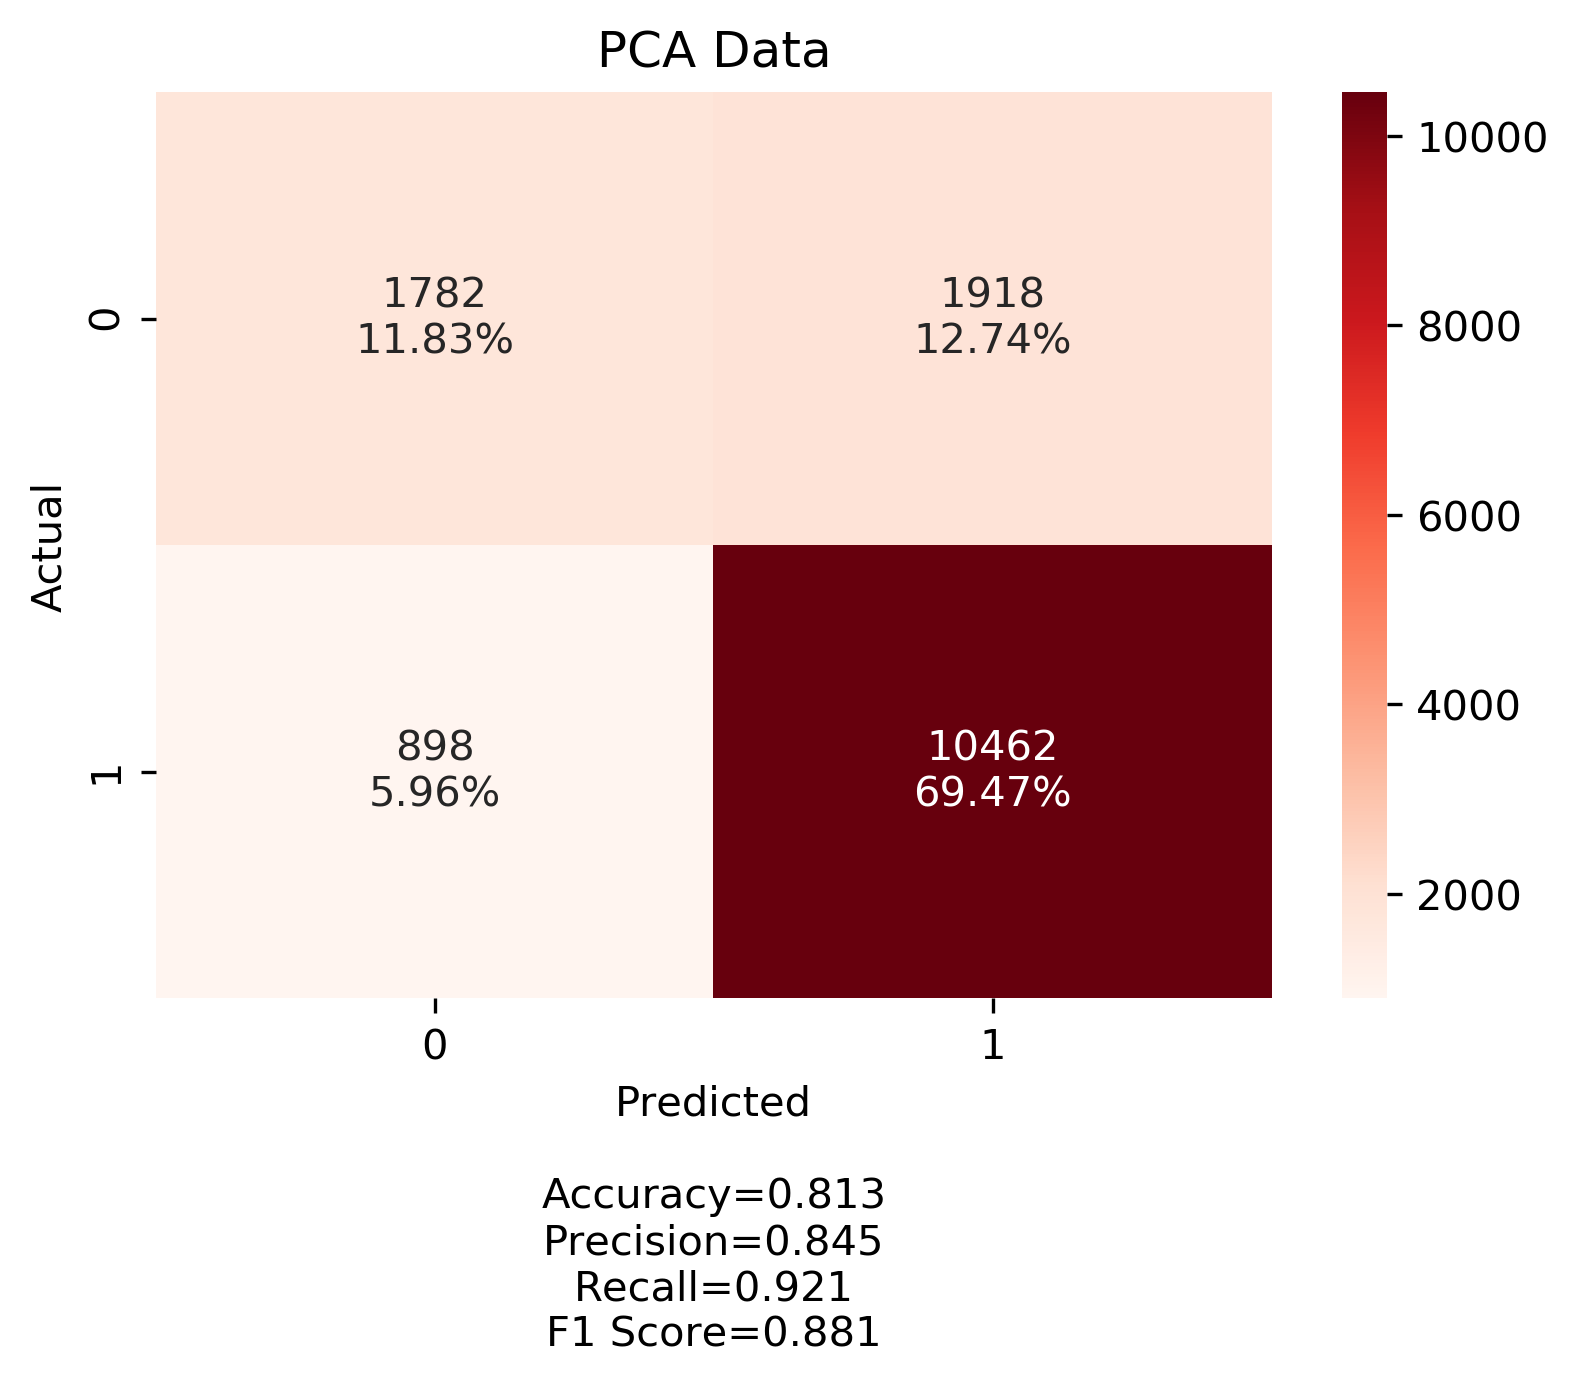
\includegraphics[width=.45\textwidth]{images/cf8.png}		
		\end{center}
		
		Things to Consider:
		\begin{itemize}
			\item Points near the separating line are difficult to \emph{confidently} classify
			\item This method should not be used on collinear data, since it has done well here, we can see that the data is not collinear (and feature selection reduces this further)
			\item Finding an approximation for $ \mathbf{w} $ can be slow and tedious on a large set of data with high dimensions
		\end{itemize}		
				
		\subsection{Linear Regression}~
		
		This technique is similar to logistical regression when used to determine an optimal $ \mathbf{w} $ for a linear separator. The difference comes in the form of how the function (\ref{sse}) is being found. With the goal being to fit a model with potential collinearity. This possible dependence does not work very well for the logistical regression data. In this case the goal is to separate based on minimizing the sum of squares formula to partition the data best.
				
		\begin{equation}\label{sse}
			SSE = \dfrac{1}{2n}\sum\limits_{i=1}^n(y_i - \mathbf{w}^T\mathbf{x}_i)^2
		\end{equation}
		
		Once found, we can then use the best found $ \mathbf{\hat w} $ to find $ \hat y_i $ predicted from the test set.
				
		\begin{equation}
		\hat y_i = \mathbf{\hat w}\cdot \mathbf{x}_i
		\end{equation}
		Running this model on our four data sets results in the following confusion matrices:
		\begin{center}
			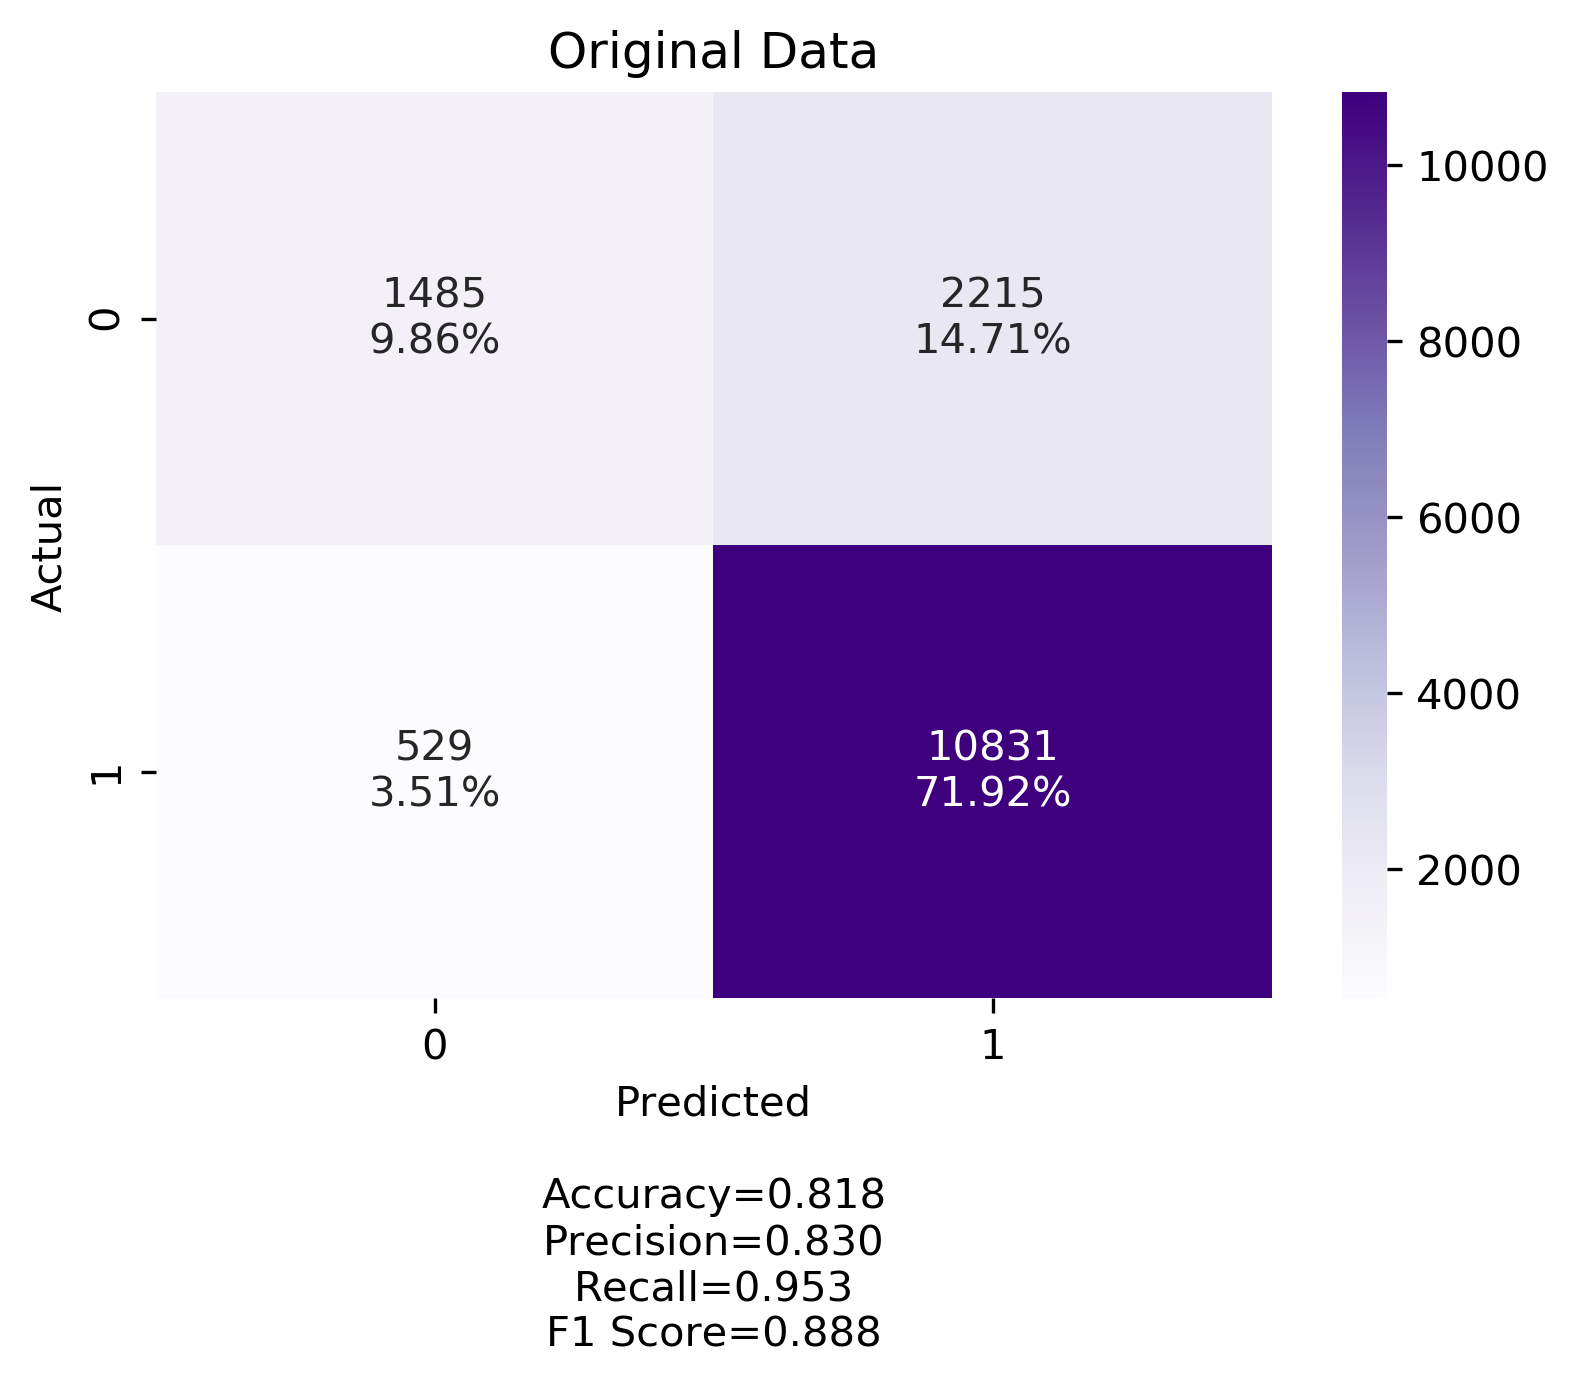
\includegraphics[width=.45\textwidth]{images/cf9.png}
			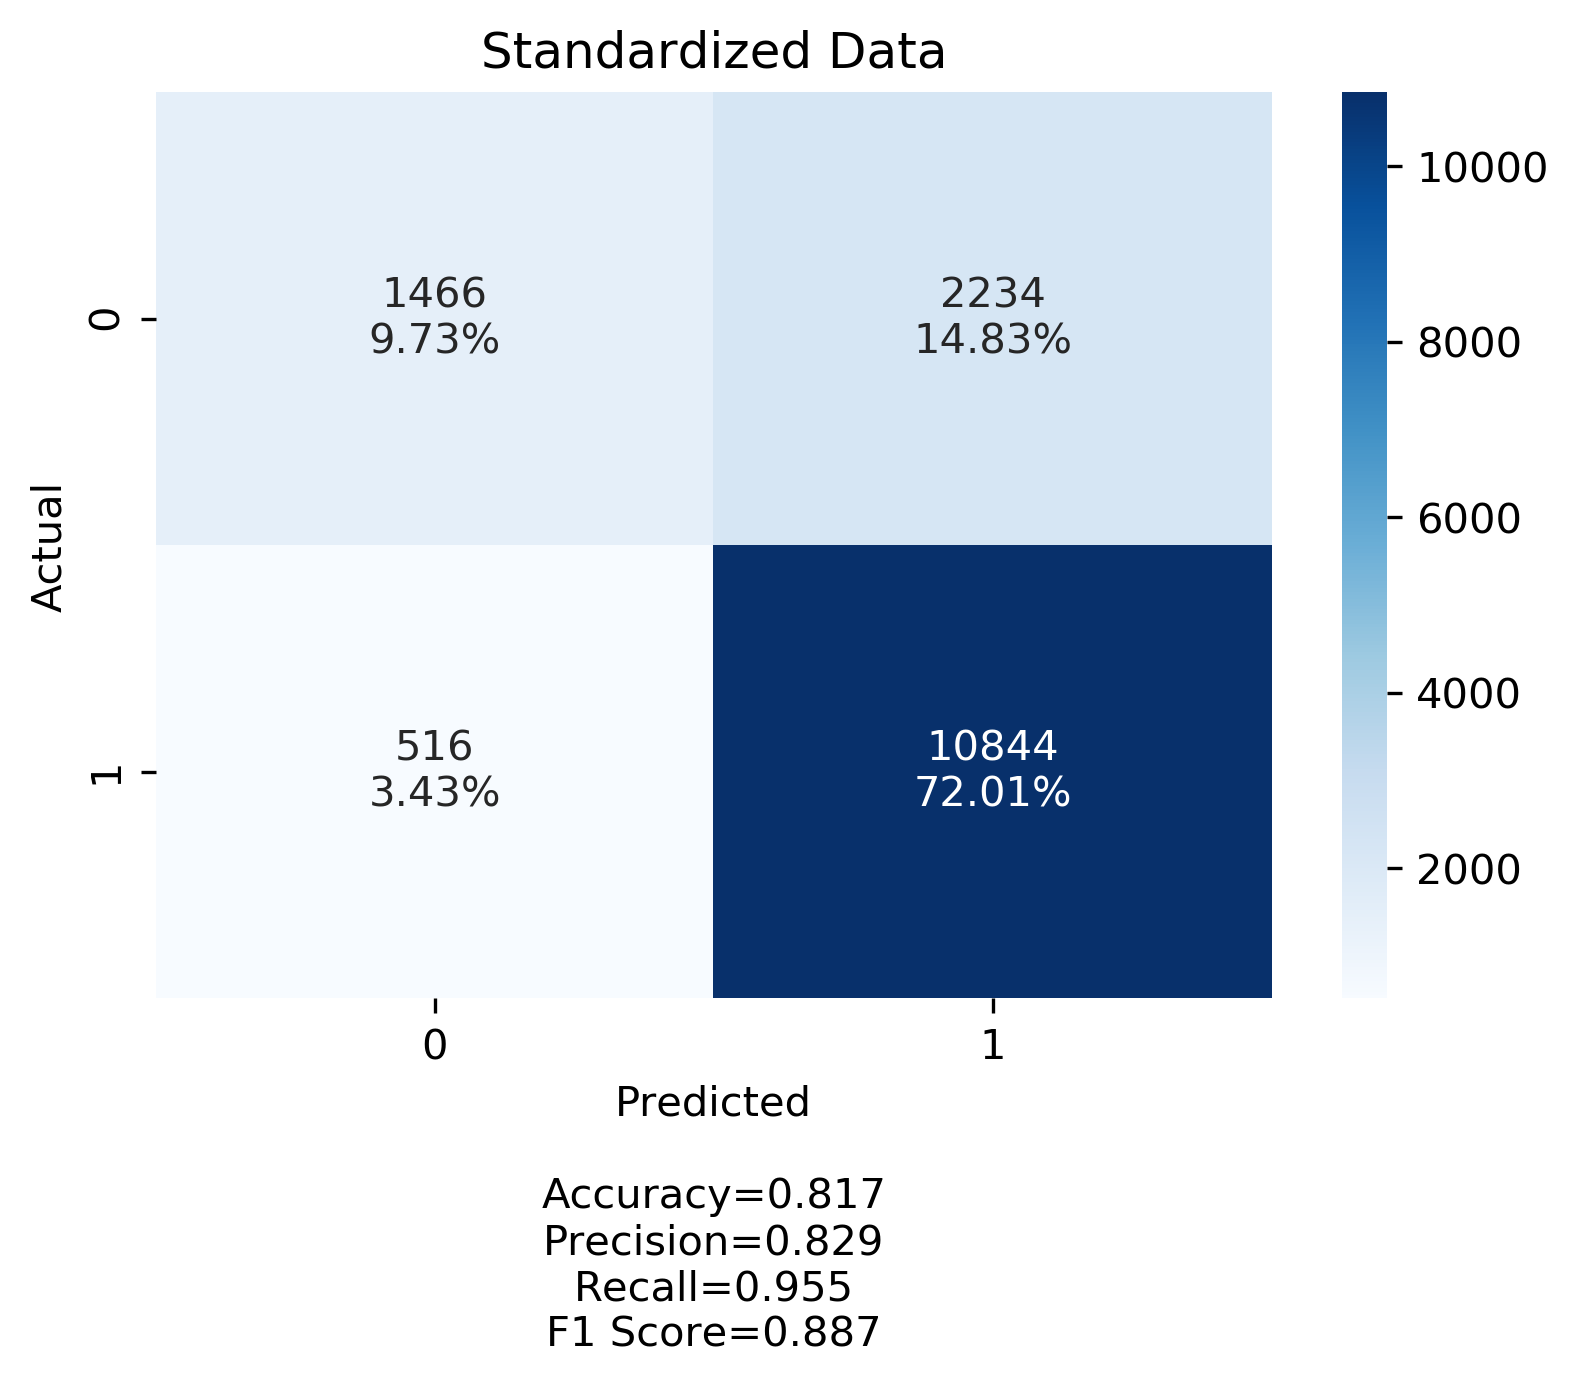
\includegraphics[width=.45\textwidth]{images/cf10.png}
			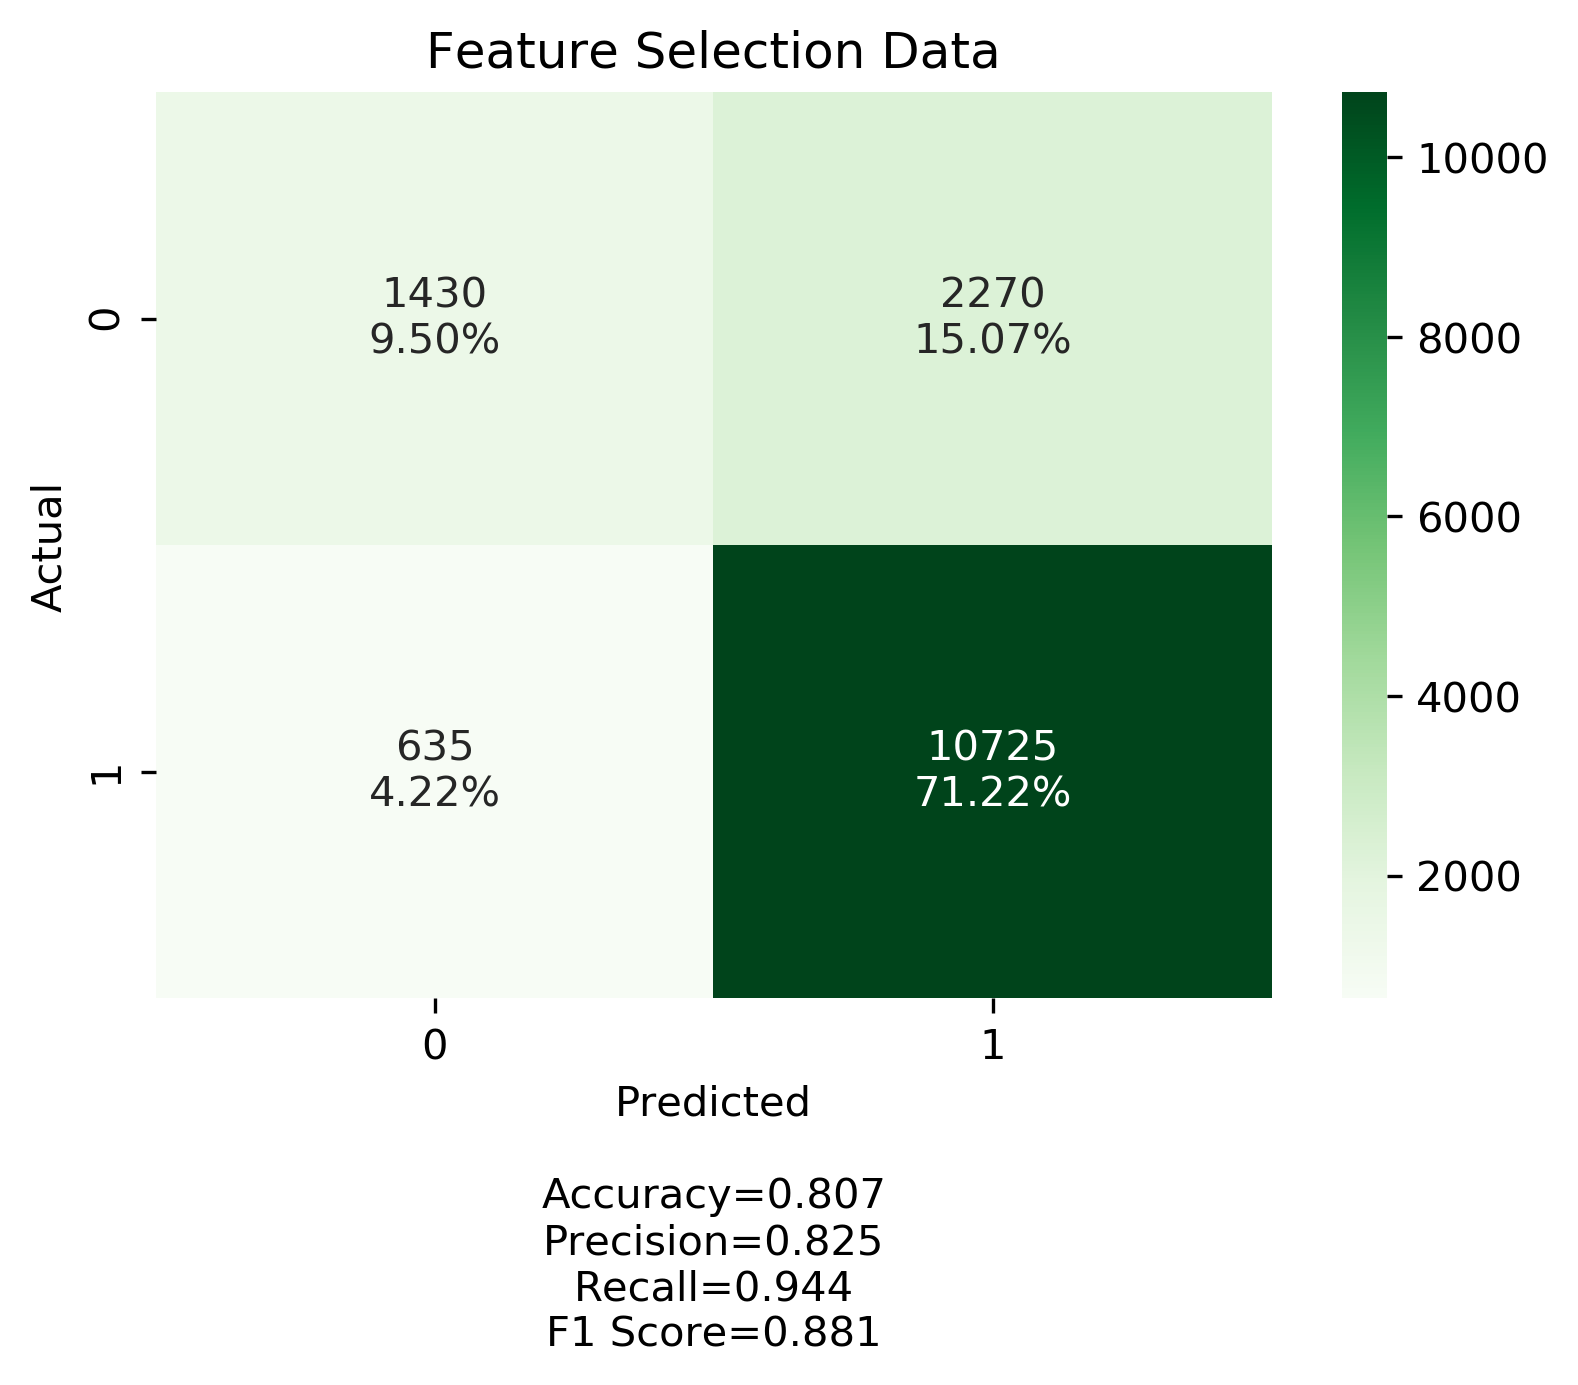
\includegraphics[width=.45\textwidth]{images/cf11.png}
			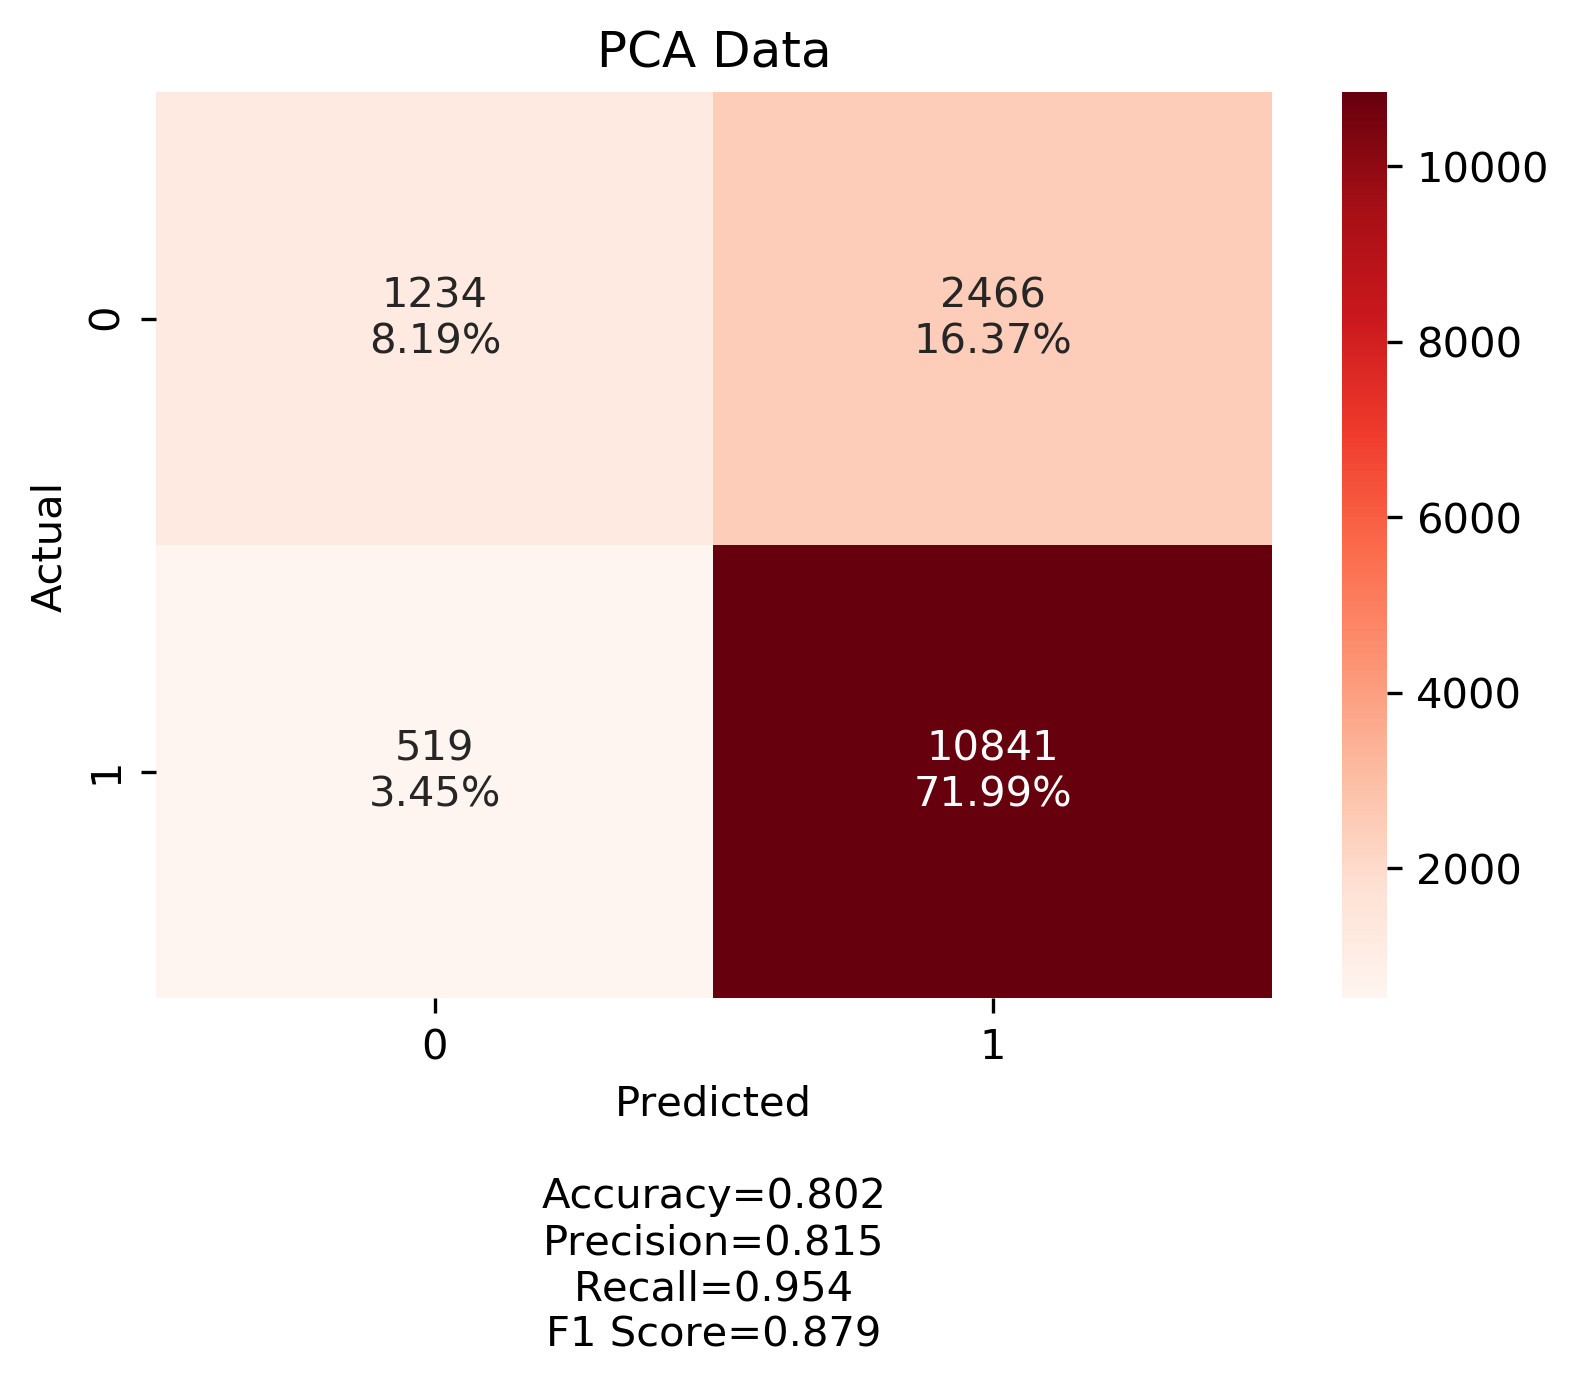
\includegraphics[width=.45\textwidth]{images/cf12.png}		
		\end{center}
		
		Things to Consider:
		\begin{itemize}
			\item This method may take a bit more time finding an optimal $ \mathbf{\hat w} $ value
			\item Better than logistical when we have potentially dependant data
		\end{itemize}		
		
		\subsection{Support Vector Machine}~
				Building on the past two logistical regression and linear regression models. The Support Vector Machine approach relies on constructing some separating line between the classified data. This minimized line that is found will have two adjacent lines to assist finding an optimal $\mathbf{w} $ value to separate the data. These two adjacent lines are called "Support Vectors". We can further apply kernel methods to this SVM to increase accuracy though for our purposes we have just implemented a basic support vector machine from \emph{sklearn}.
				
				This function (\ref{svm_eq}) is used to find $\mathbf{\hat w}$.
				
				\begin{equation}\label{svm_eq}
					y_i(\mathbf{ w} \cdot \mathbf{x}_i + b) = 1-\hat\xi
				\end{equation}
				$ \hat \xi =$  error term based on support vector\\
				
		Running this model on our four data sets results in the following confusion matrices:
		\begin{center}
			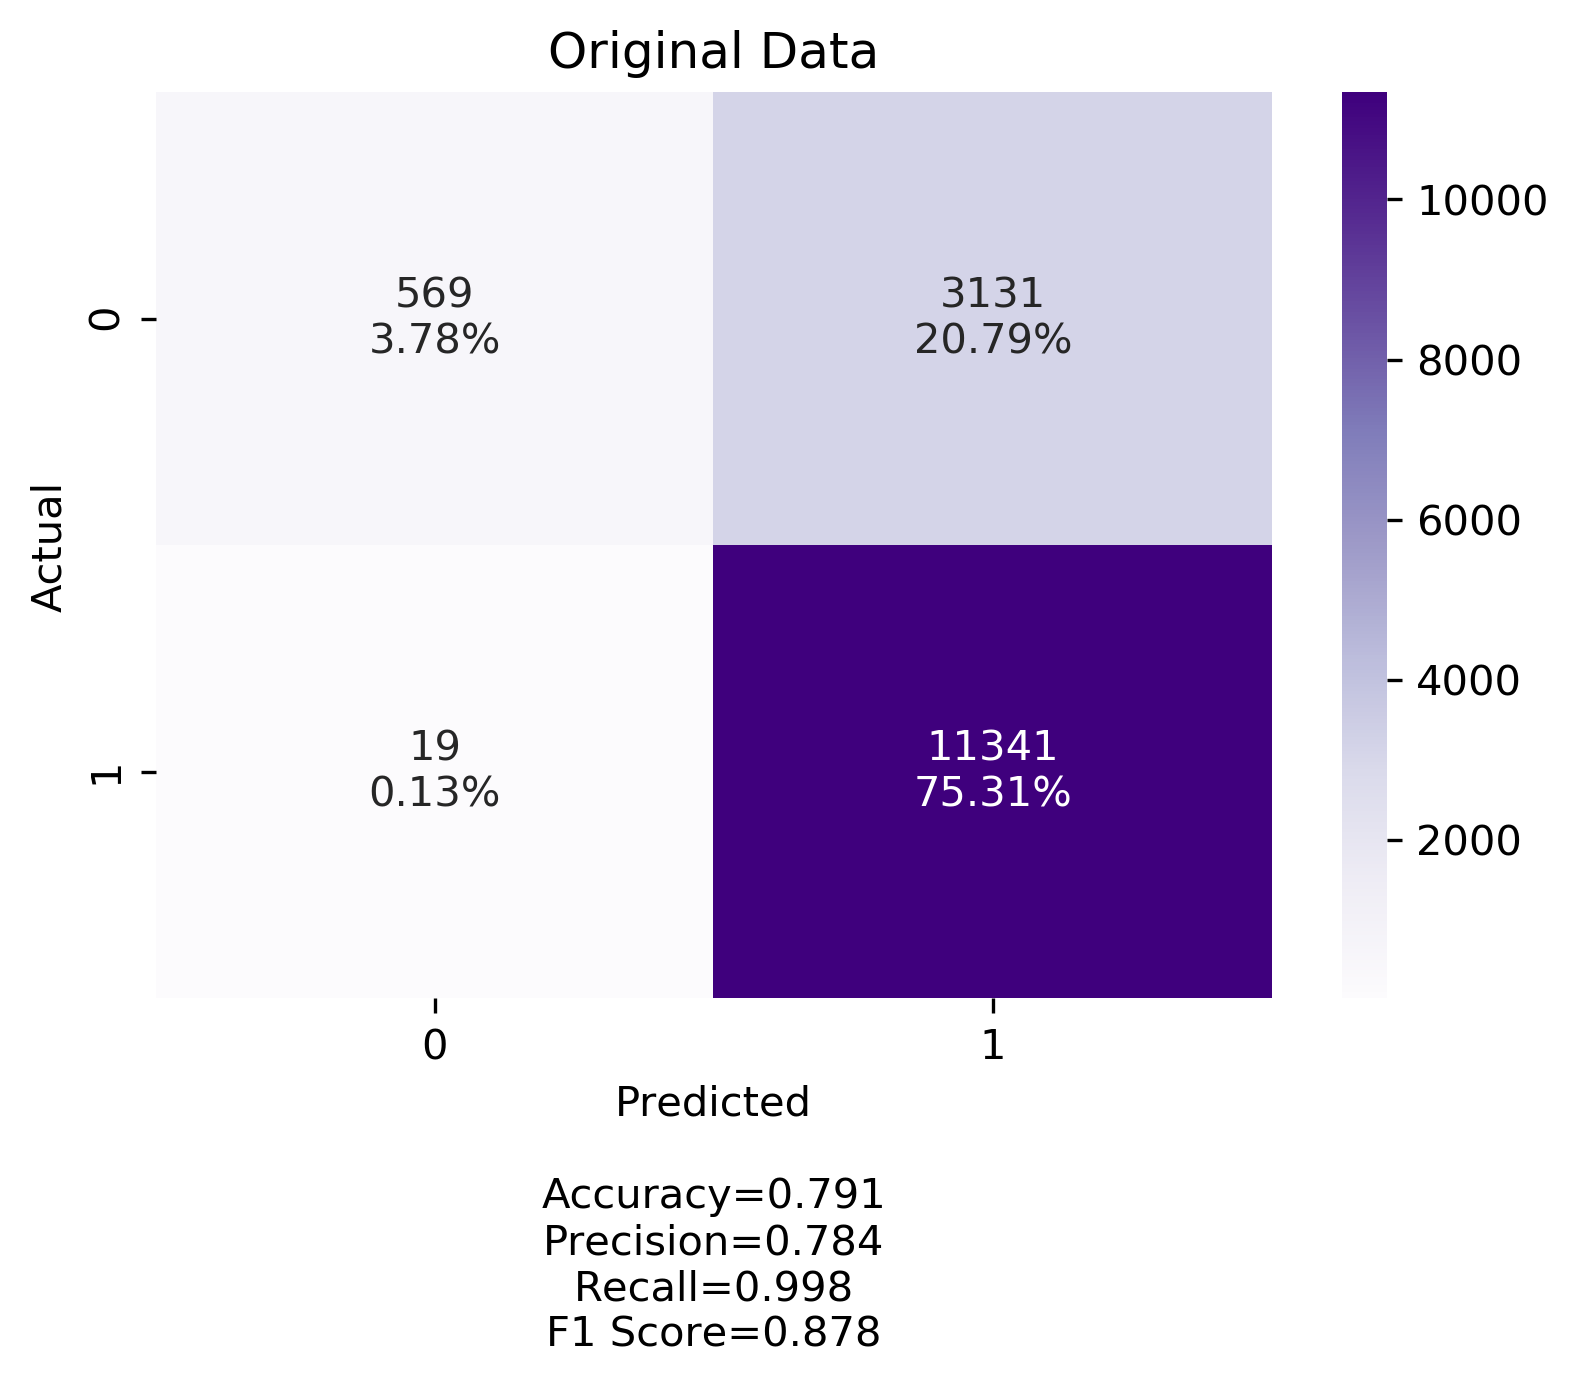
\includegraphics[width=.45\textwidth]{images/cf13.png}
			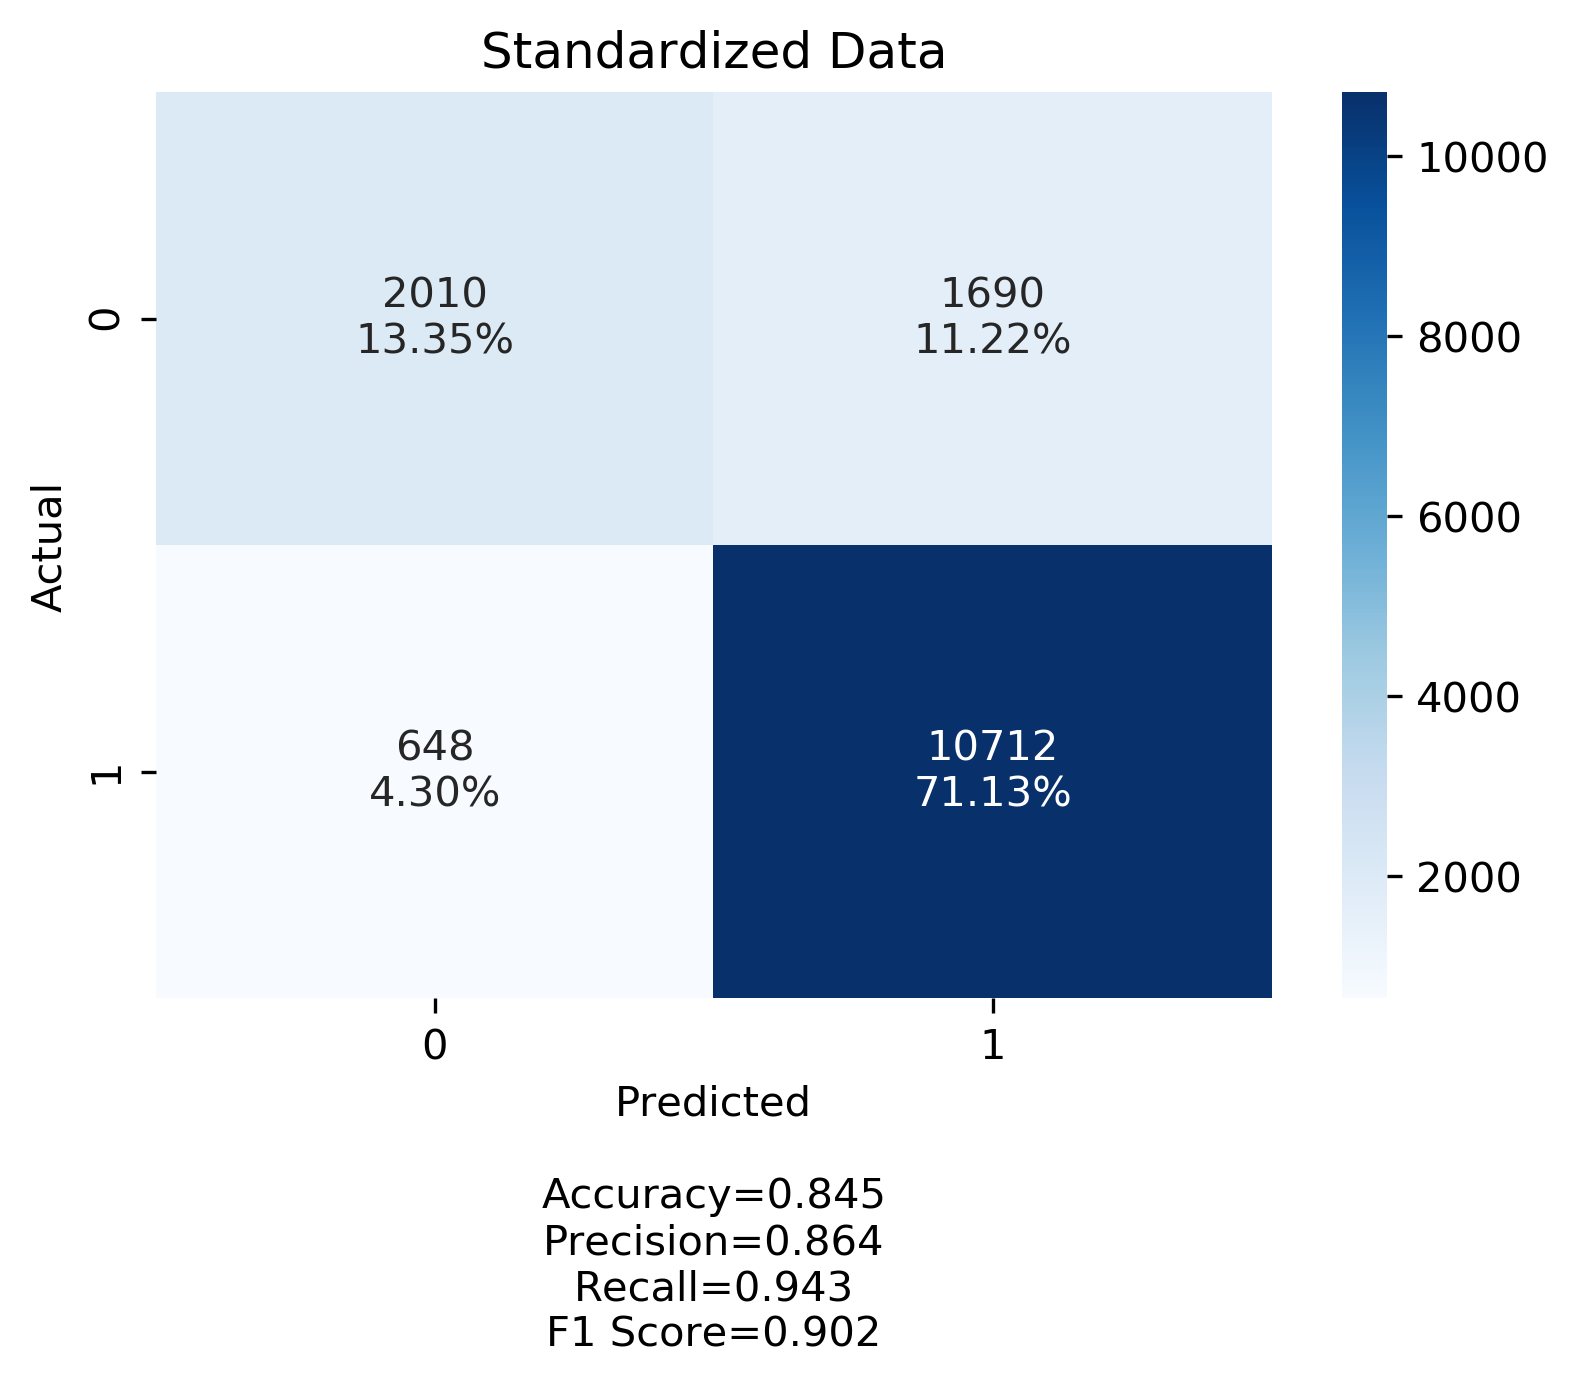
\includegraphics[width=.45\textwidth]{images/cf14.png}
			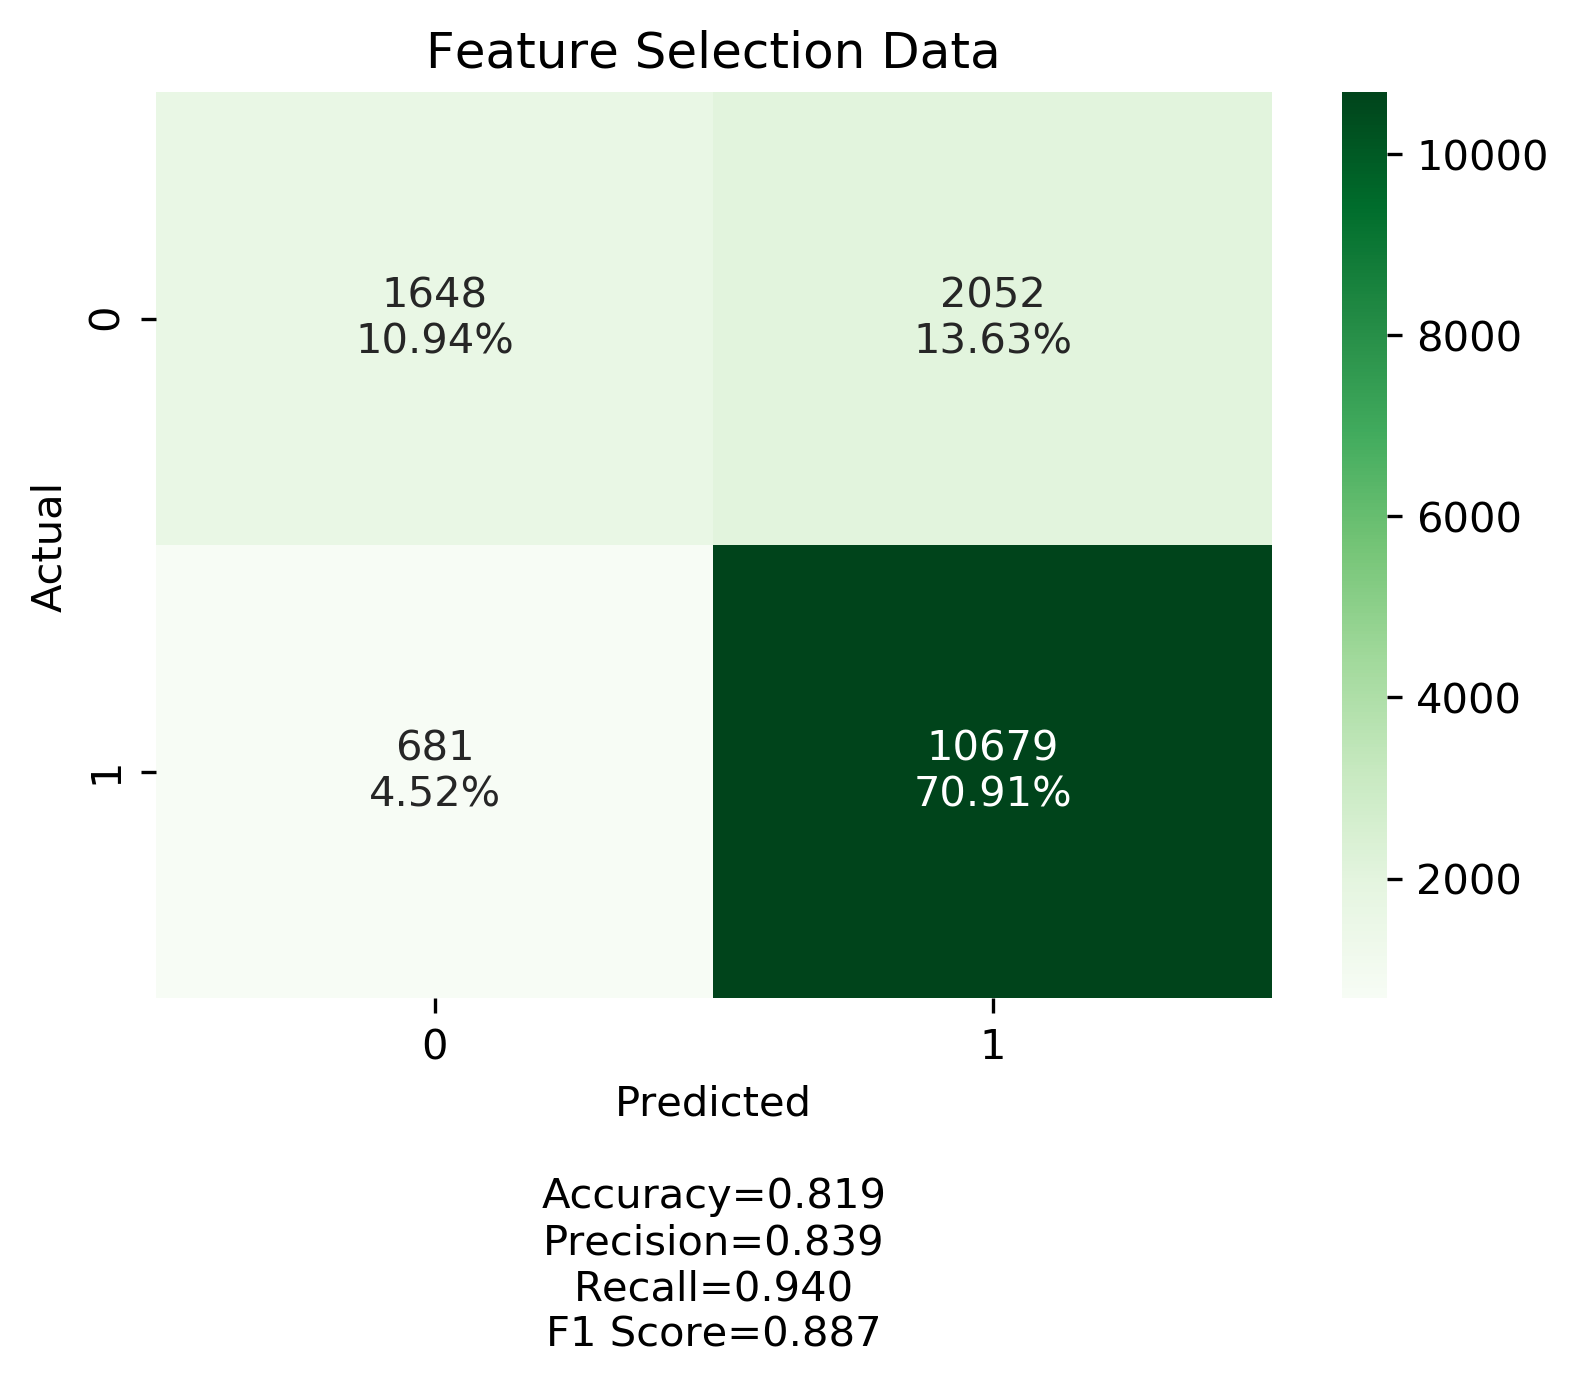
\includegraphics[width=.45\textwidth]{images/cf15.png}
			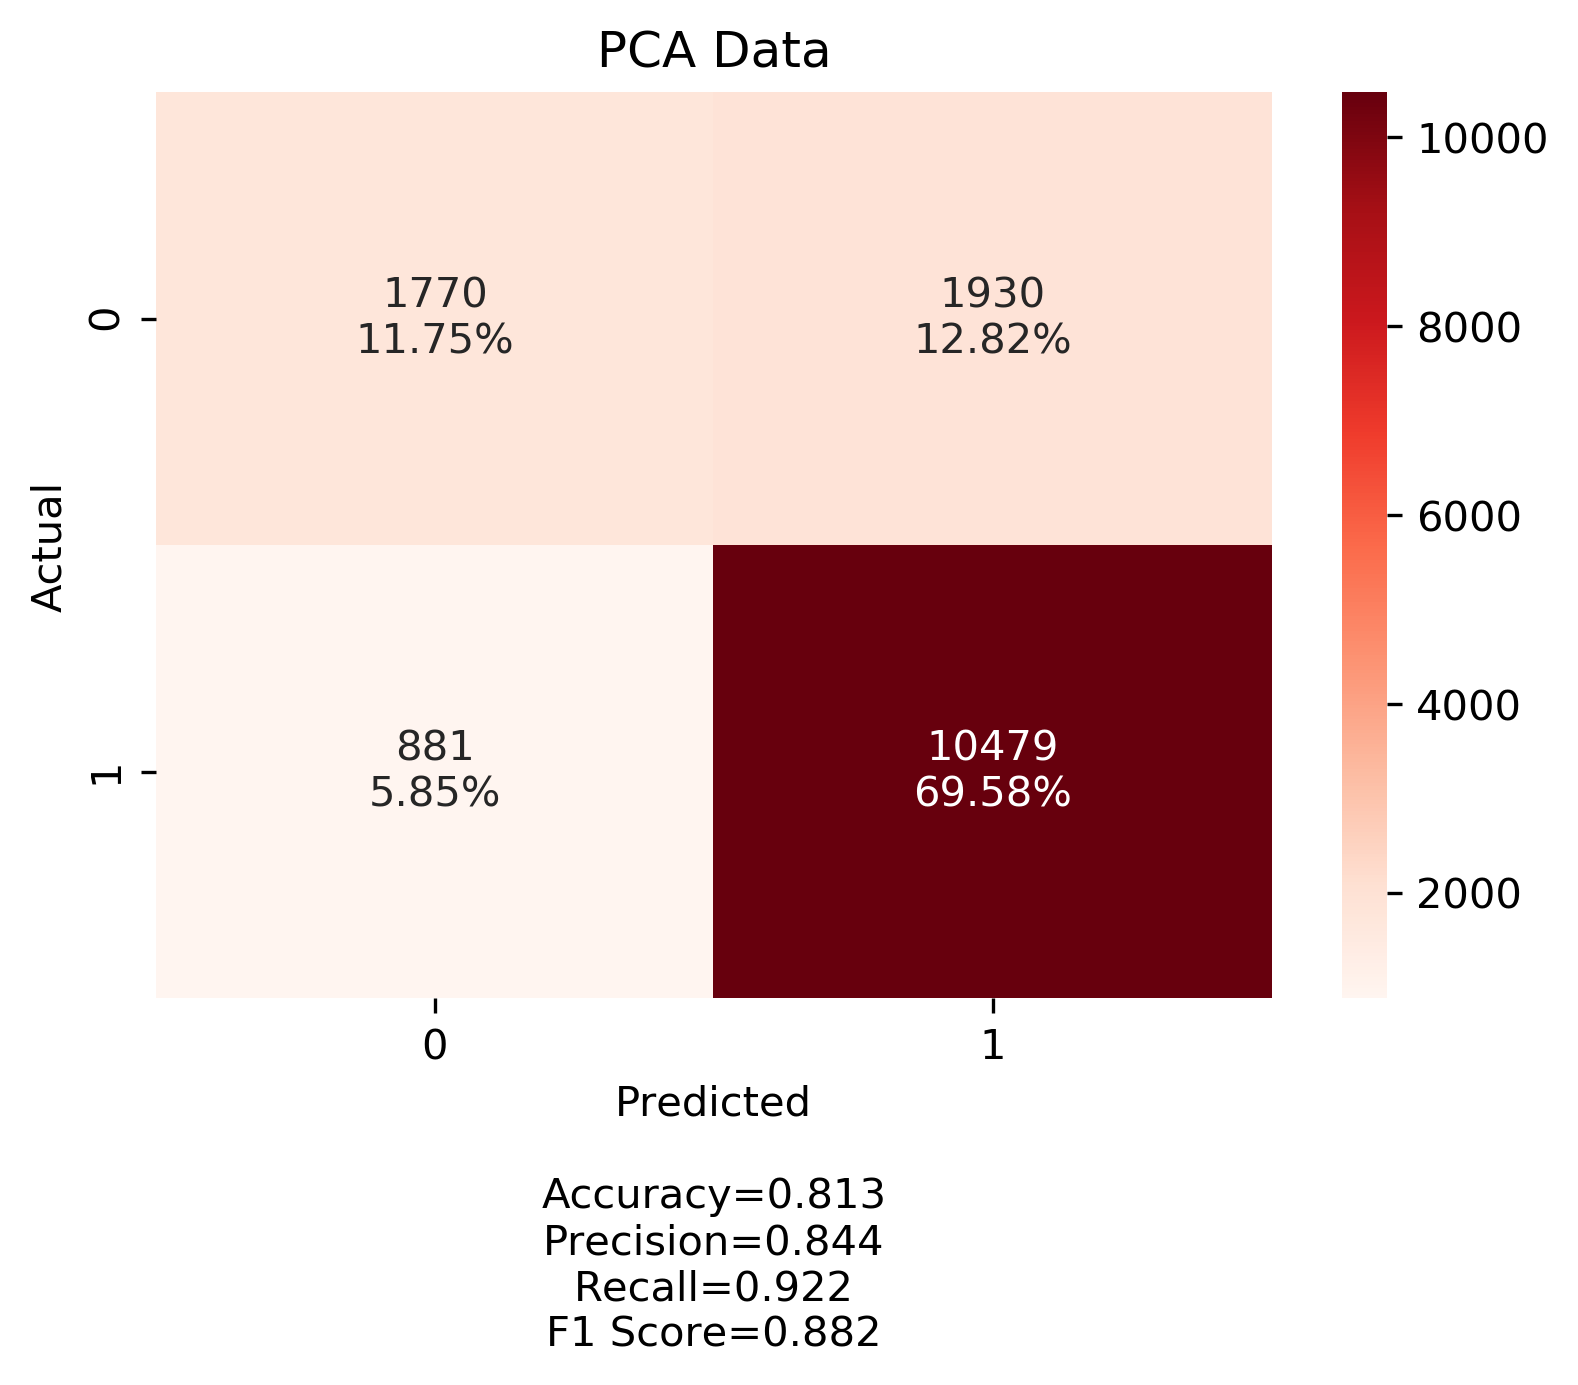
\includegraphics[width=.45\textwidth]{images/cf16.png}		
		\end{center}
		
		Things to Consider:
		\begin{itemize}
			\item If data is not easily separable may need to transform data to higher dimensions (this was the case for our data set, which we will discuss later)
			\item Best marginal points may be difficult to choose (causing poor support vector)
		\end{itemize}		
		
		
		\subsection{Decision Tree}~
				
				This classifying algorithm uses a preprocessed tree of boolean yes/no decisions to narrow down if a person makes more or less than $ \$50000 $. This is created based on an entropy measure on every possible attribute. Choosing the attribute which causes the least amount of information loss (optimal root) we then determine the lower levels of the tree, until an adequate model has been fitted.

				\begin{equation}
					entropy(p_1,p_2,...,p_k) = \text{-}p_1 \ln{p_1}-p_2 \ln{p_2}-...-p_k \ln{p_k}
				\end{equation}
				
		Running this model on our four data sets results in the following confusion matrices:
		\begin{center}
			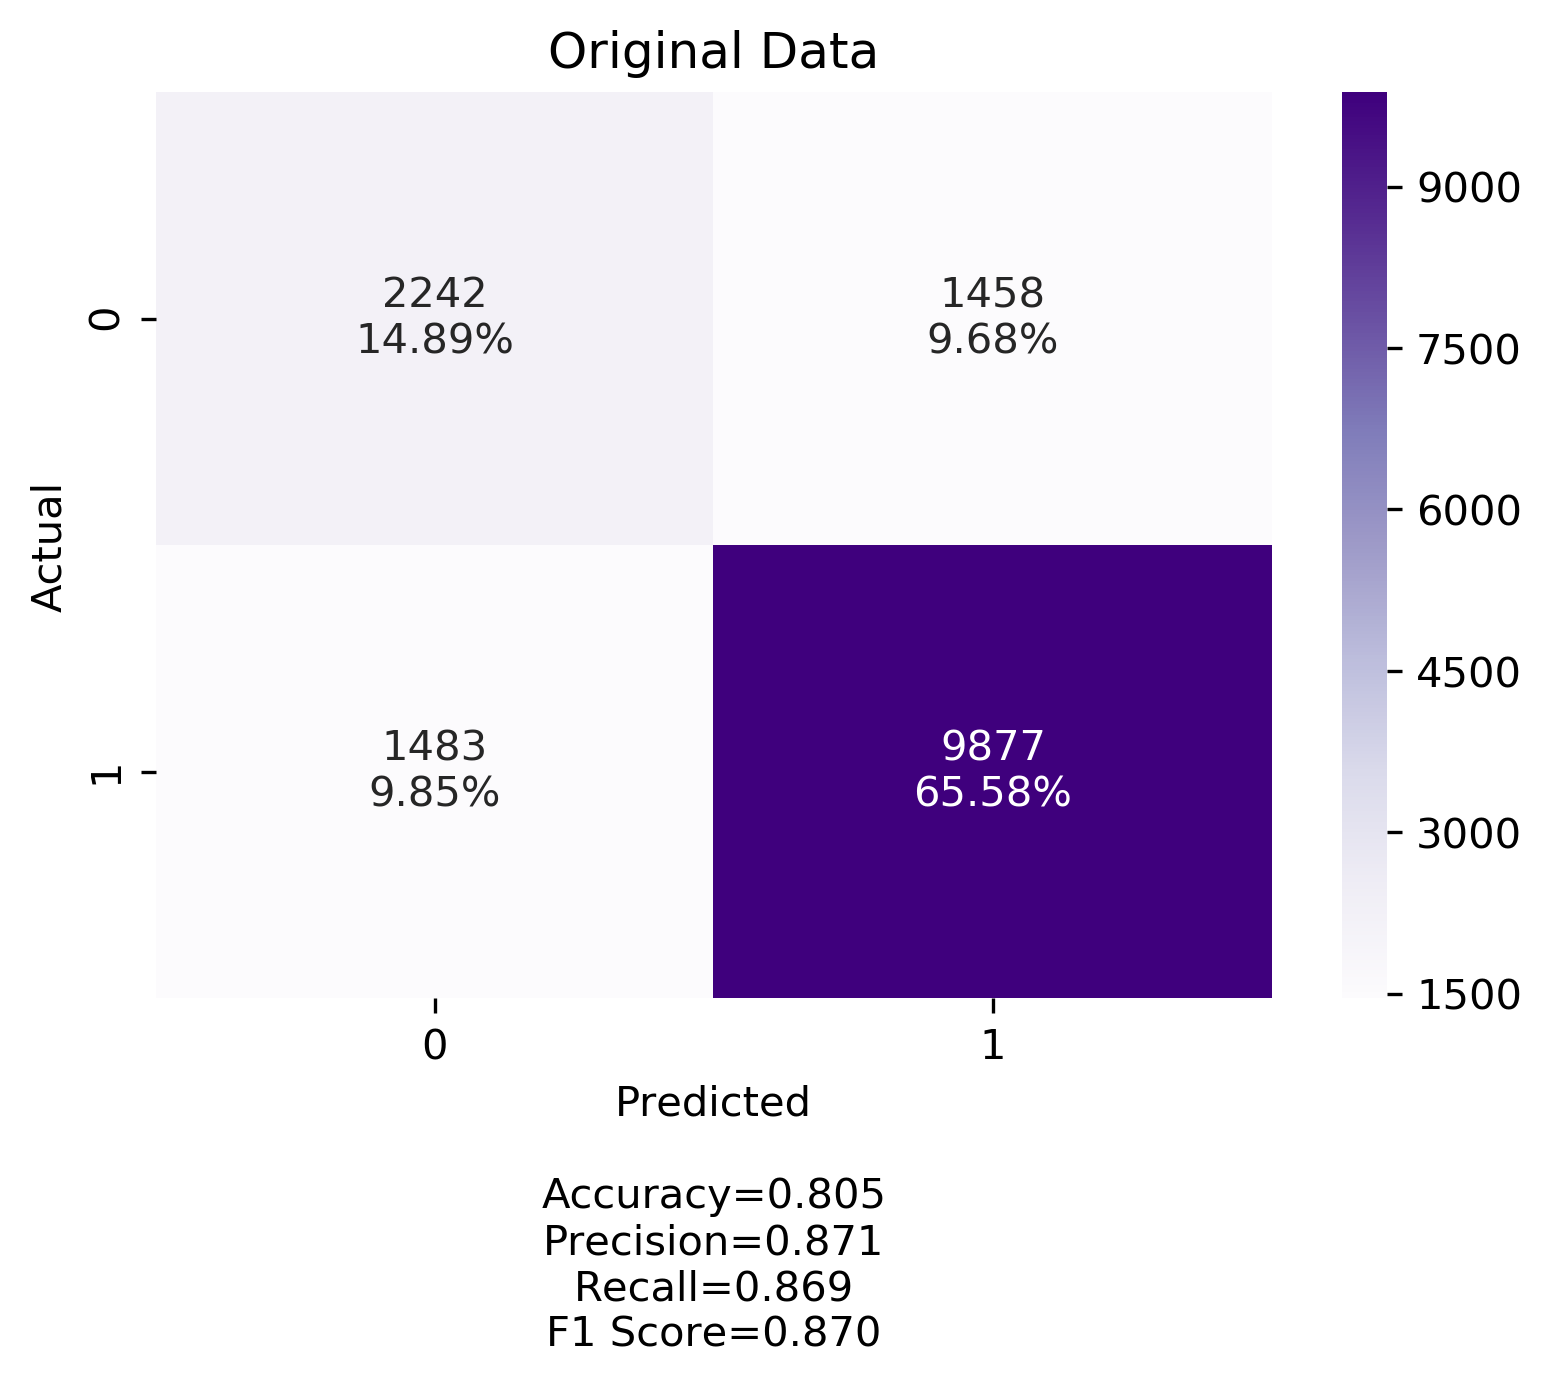
\includegraphics[width=.45\textwidth]{images/cf17.png}
			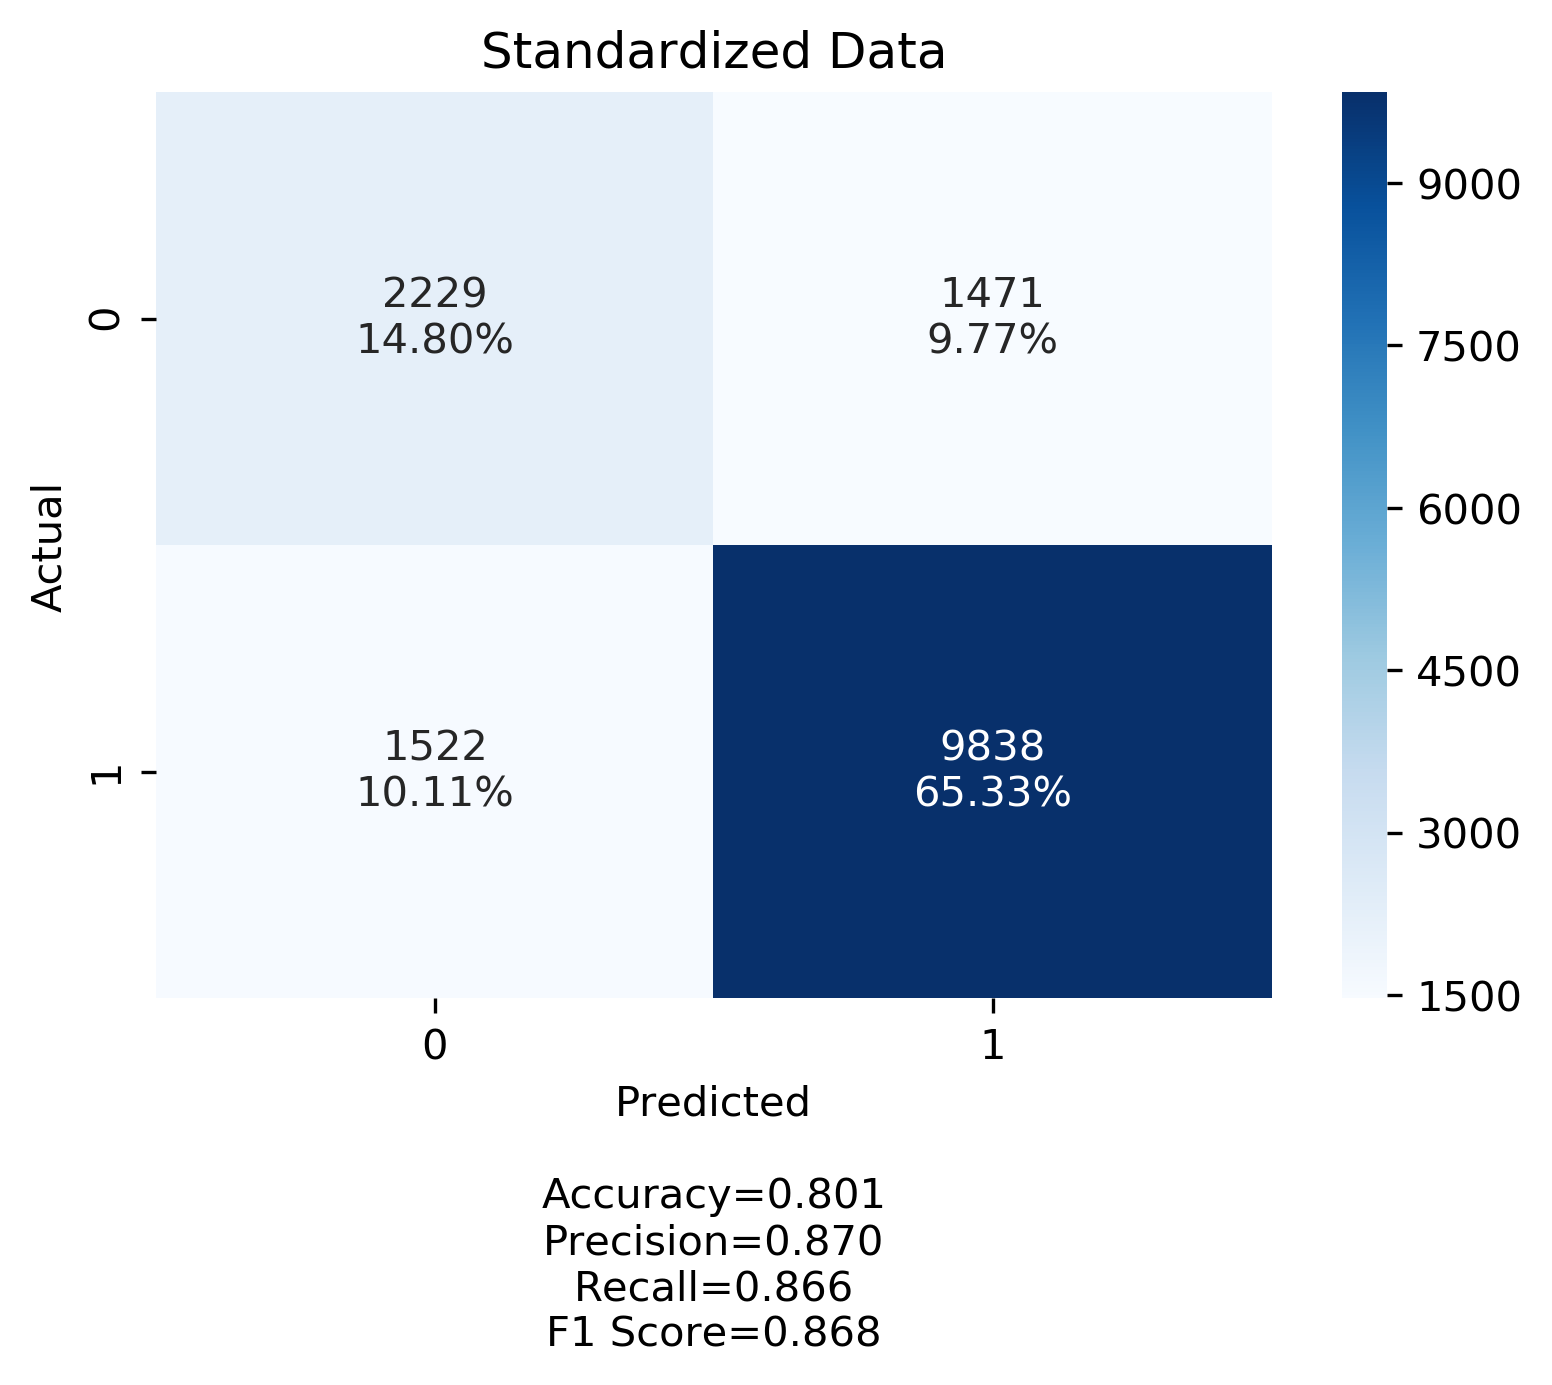
\includegraphics[width=.45\textwidth]{images/cf18.png}
			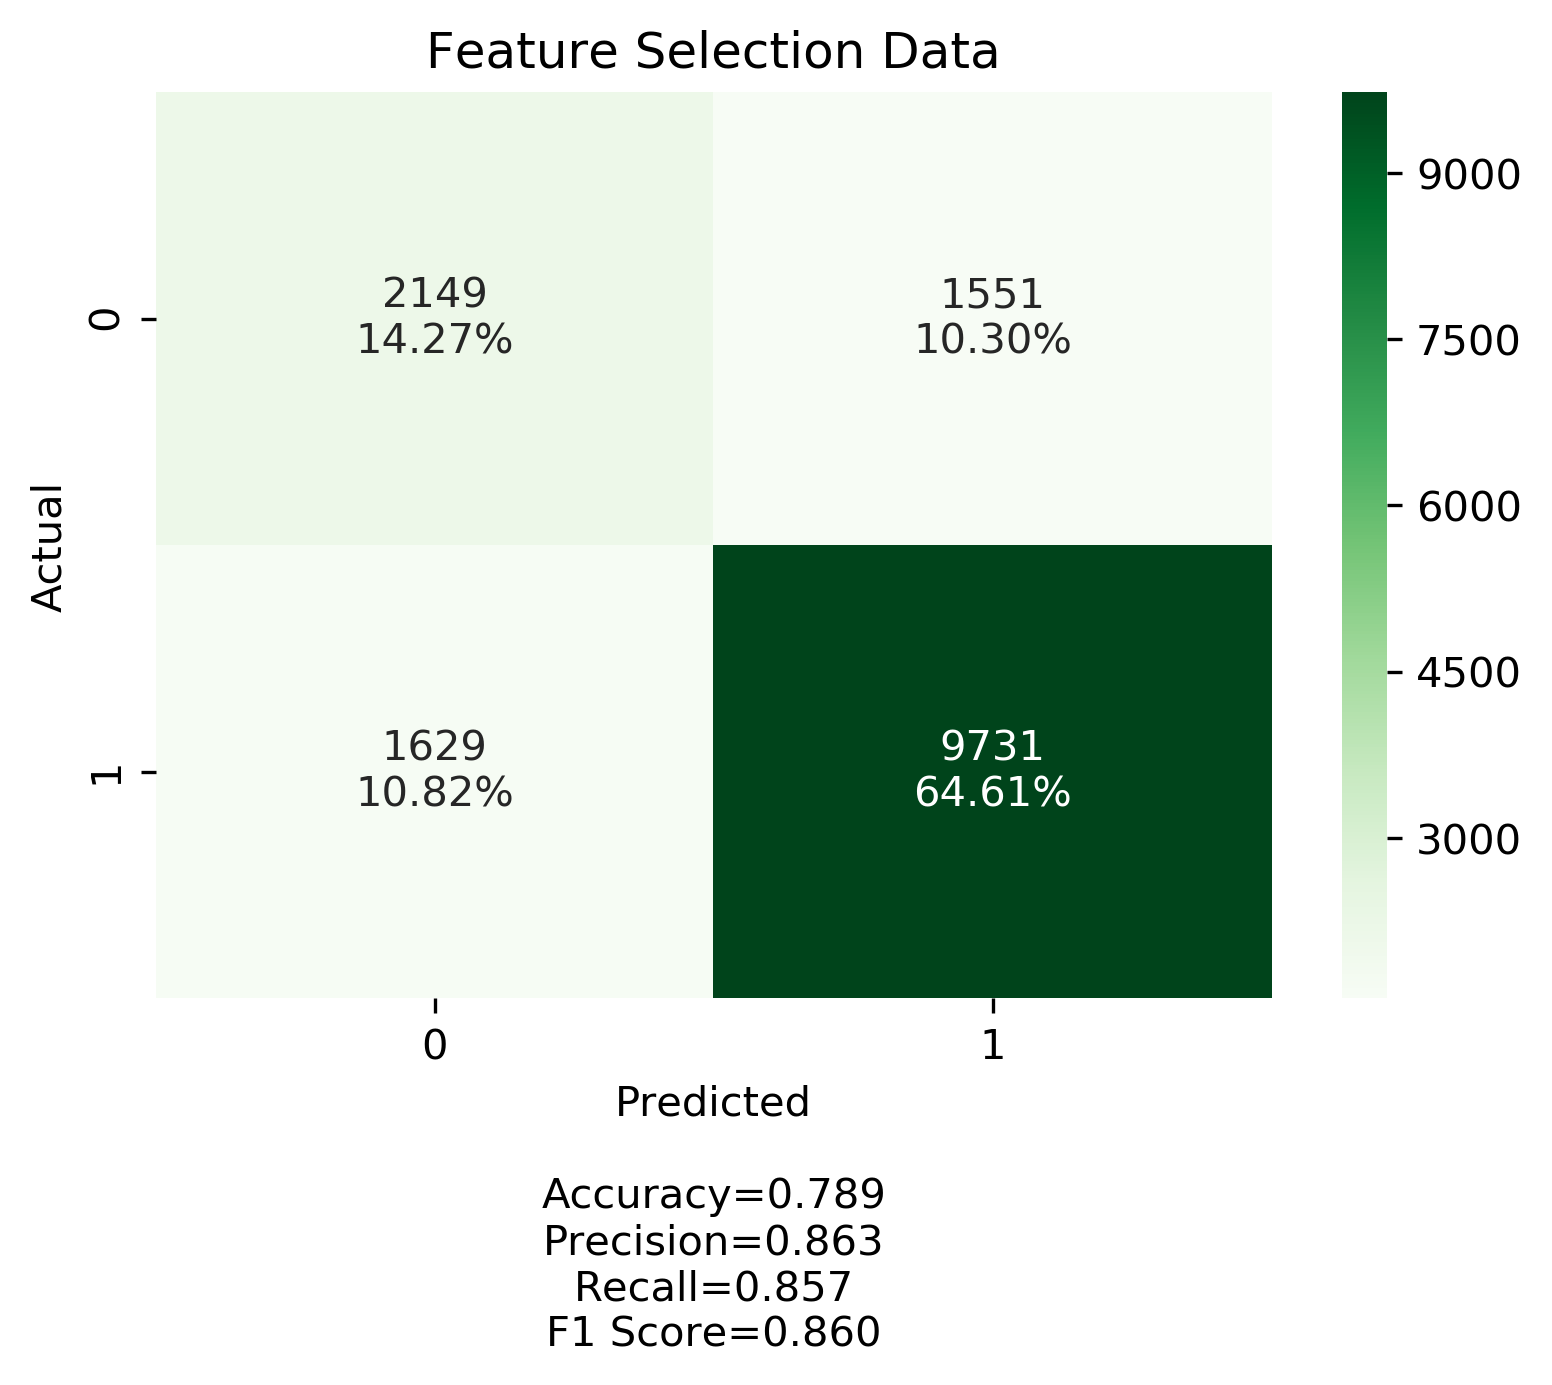
\includegraphics[width=.45\textwidth]{images/cf19.png}
			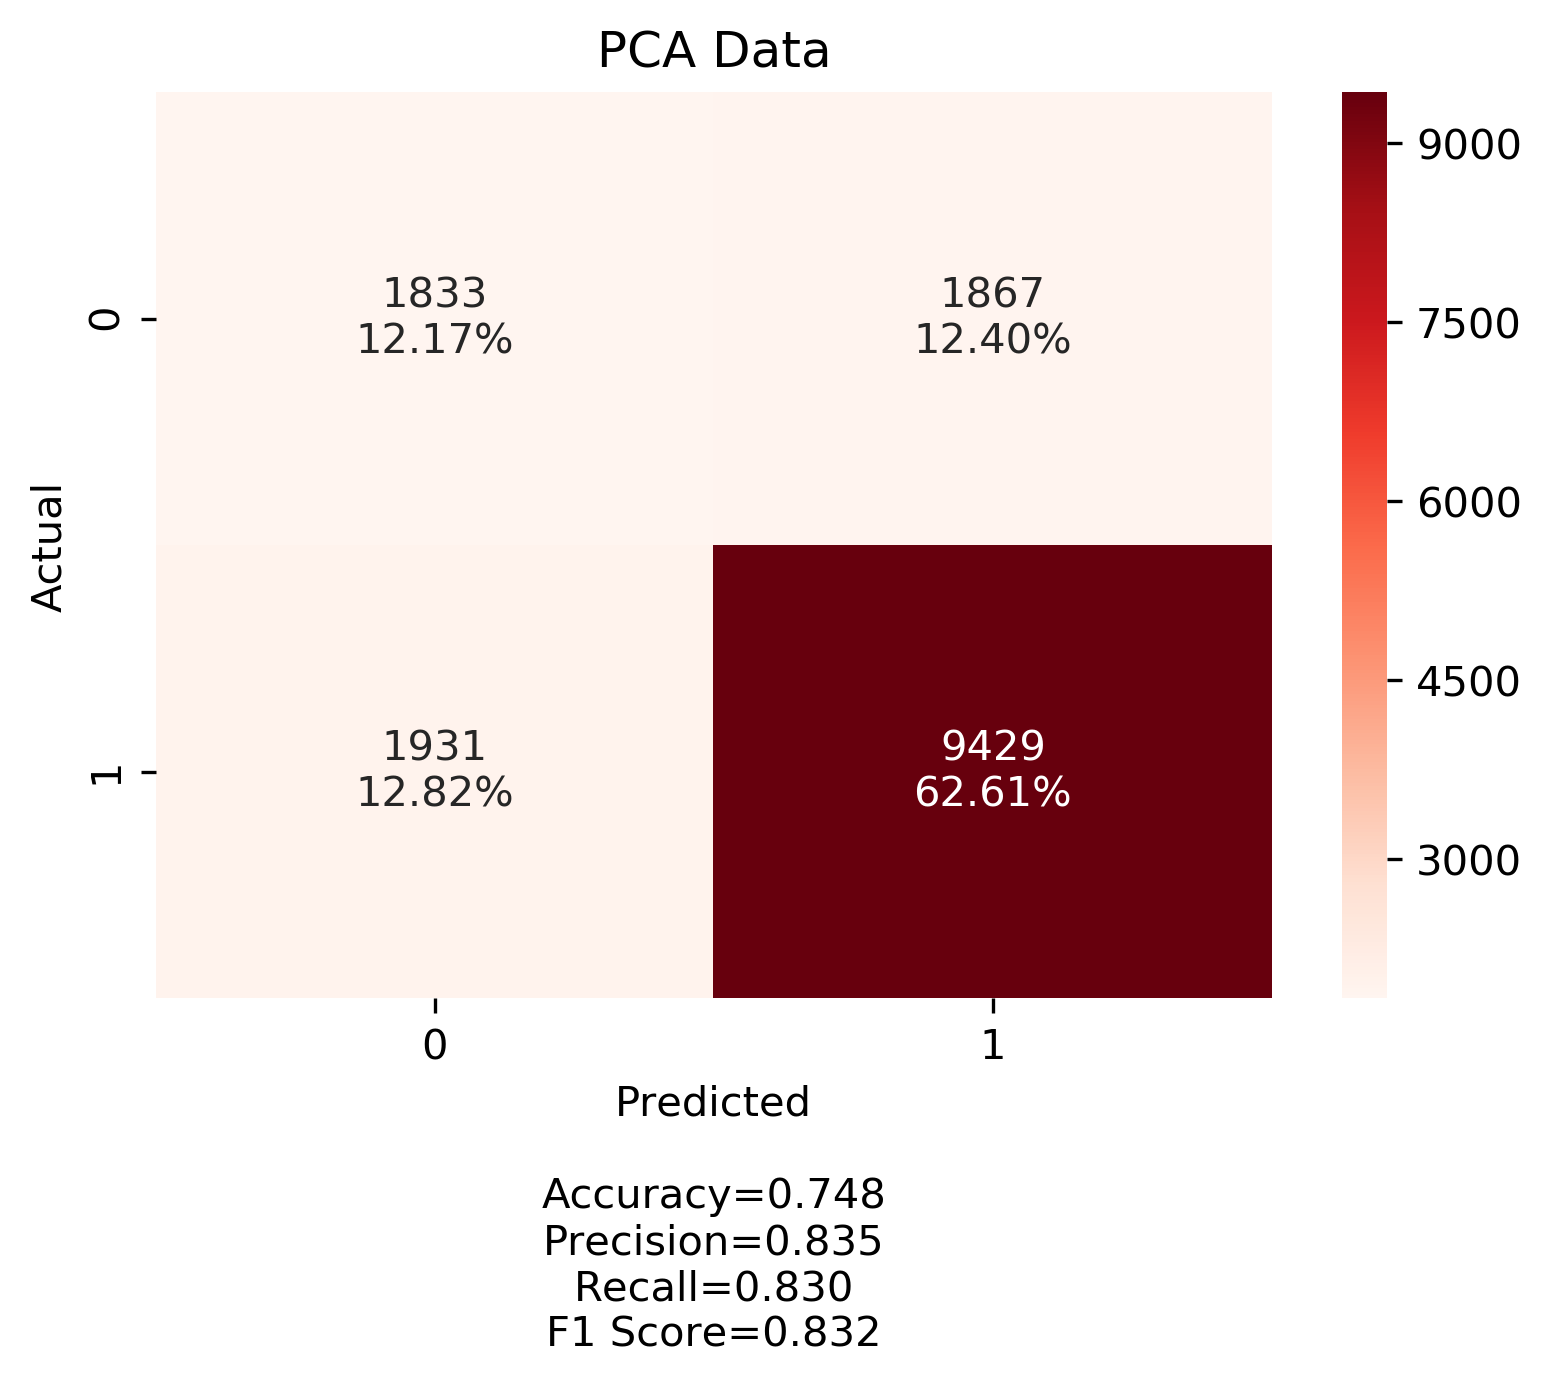
\includegraphics[width=.45\textwidth]{images/cf20.png}		
		\end{center}
		
		Things to Consider:
		\begin{itemize}
			\item Very limited with numerical data given multiple different ranges may be possible to fit data best
			\item May sometimes over fit the data (creating a tree larger than necessary)
			\item Pre/Post pruning may be necessary to optimize results (without over fitting)
		\end{itemize}		
		
		
		\subsection{Random Forest}~
			This method is building on the decision tree model. The approach is done by creating multiple smaller decision trees, then running the data through them. The eventual goal is to find a tree or group of trees that fit the data best, returning the averaged model output. When experimenting with different values, we found that setting the number of trees to 100 and setting the max depth to 20 produced good results. Running this model on our four data sets results in the following confusion matrices:
		\begin{center}
			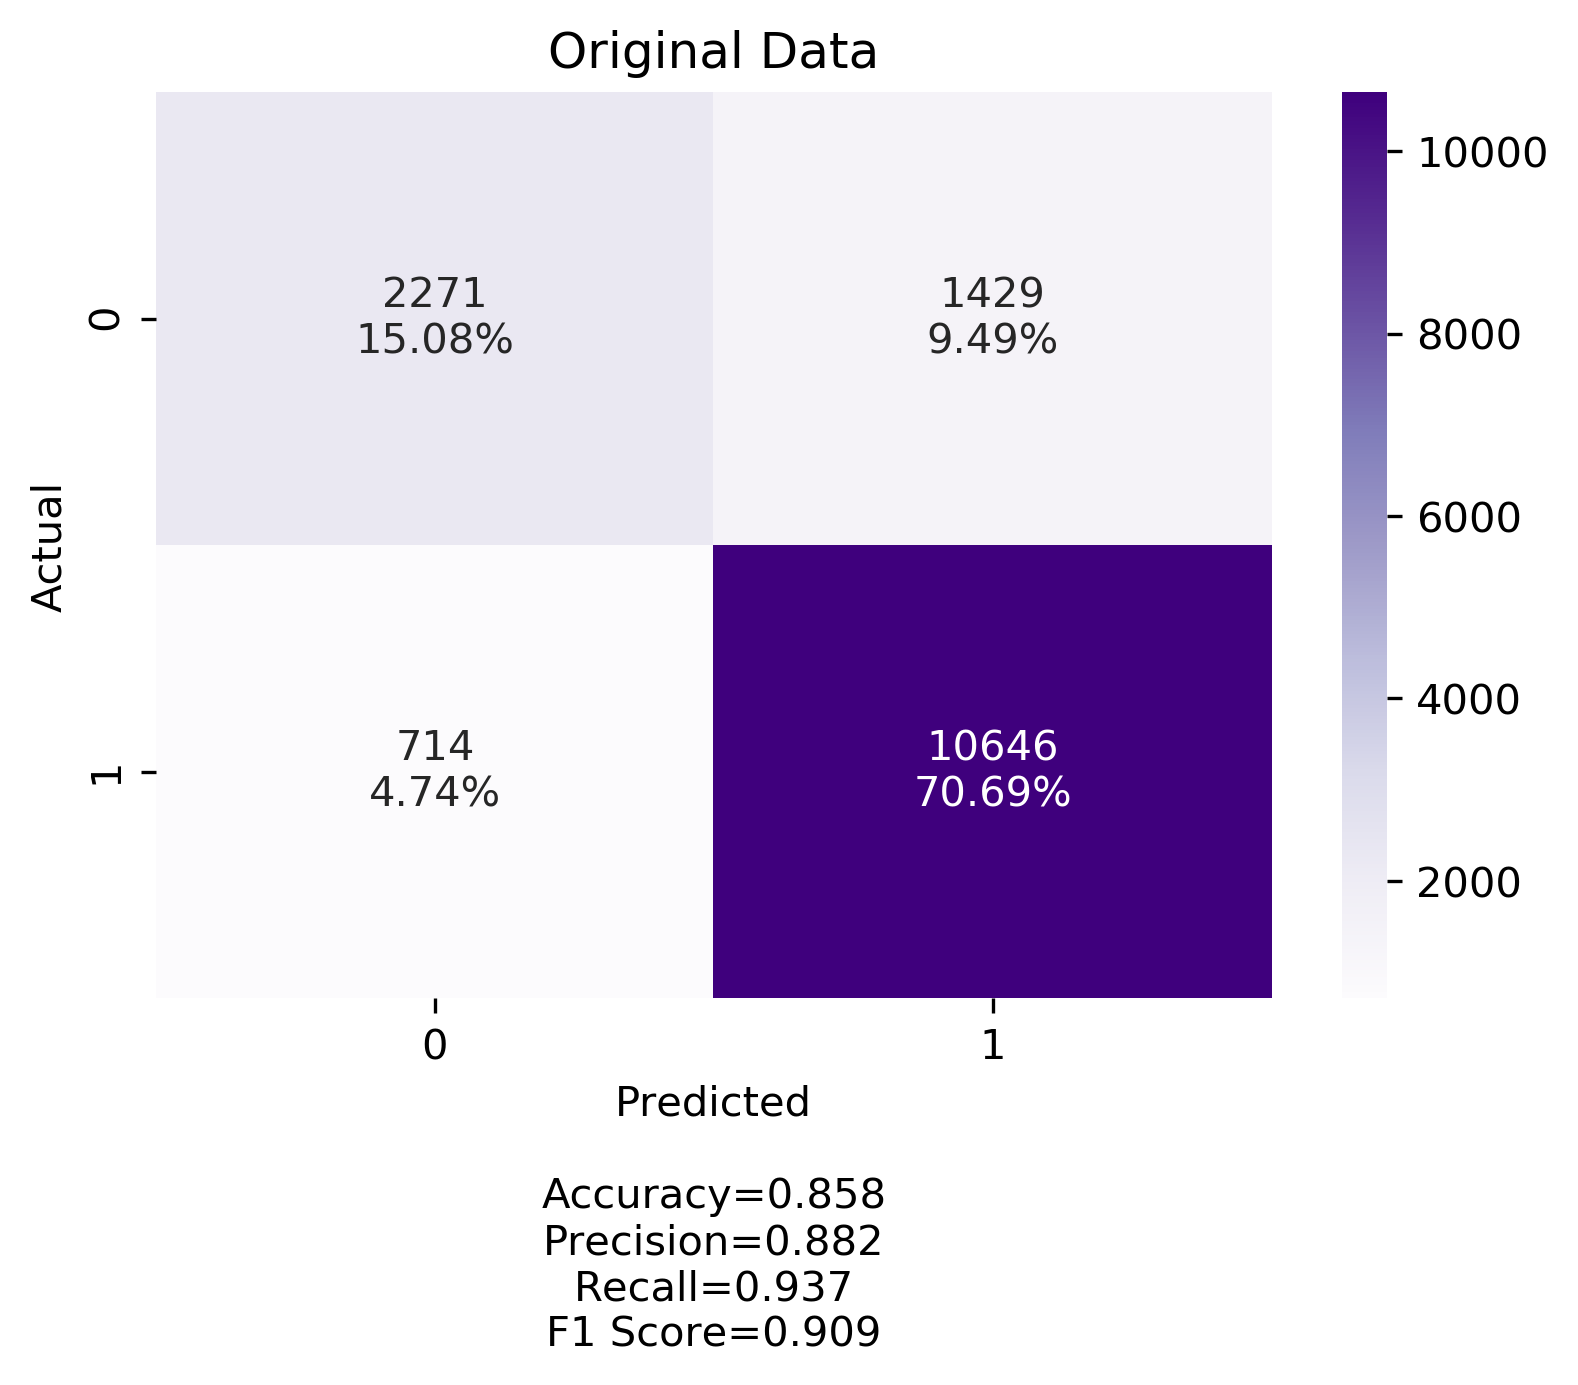
\includegraphics[width=.45\textwidth]{images/cf21.png}
			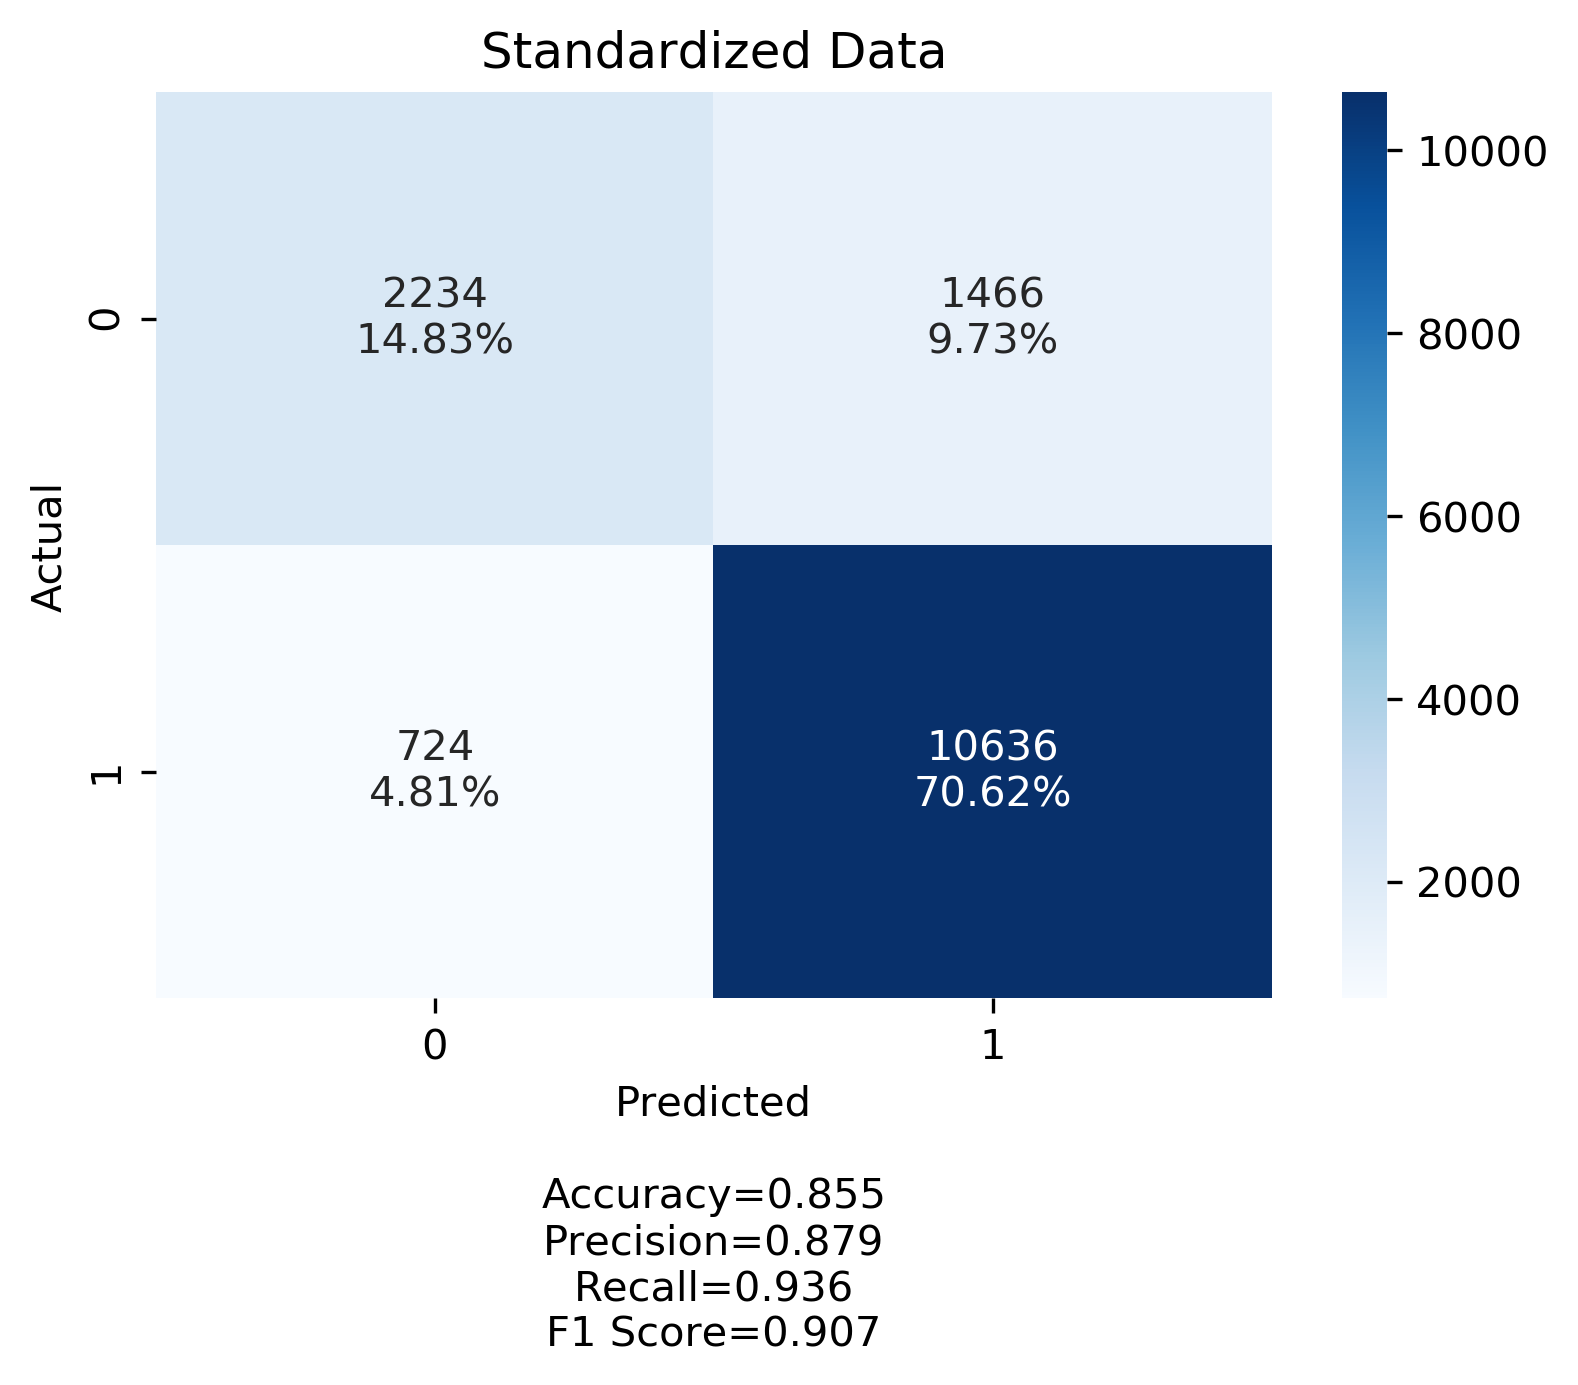
\includegraphics[width=.45\textwidth]{images/cf22.png}
			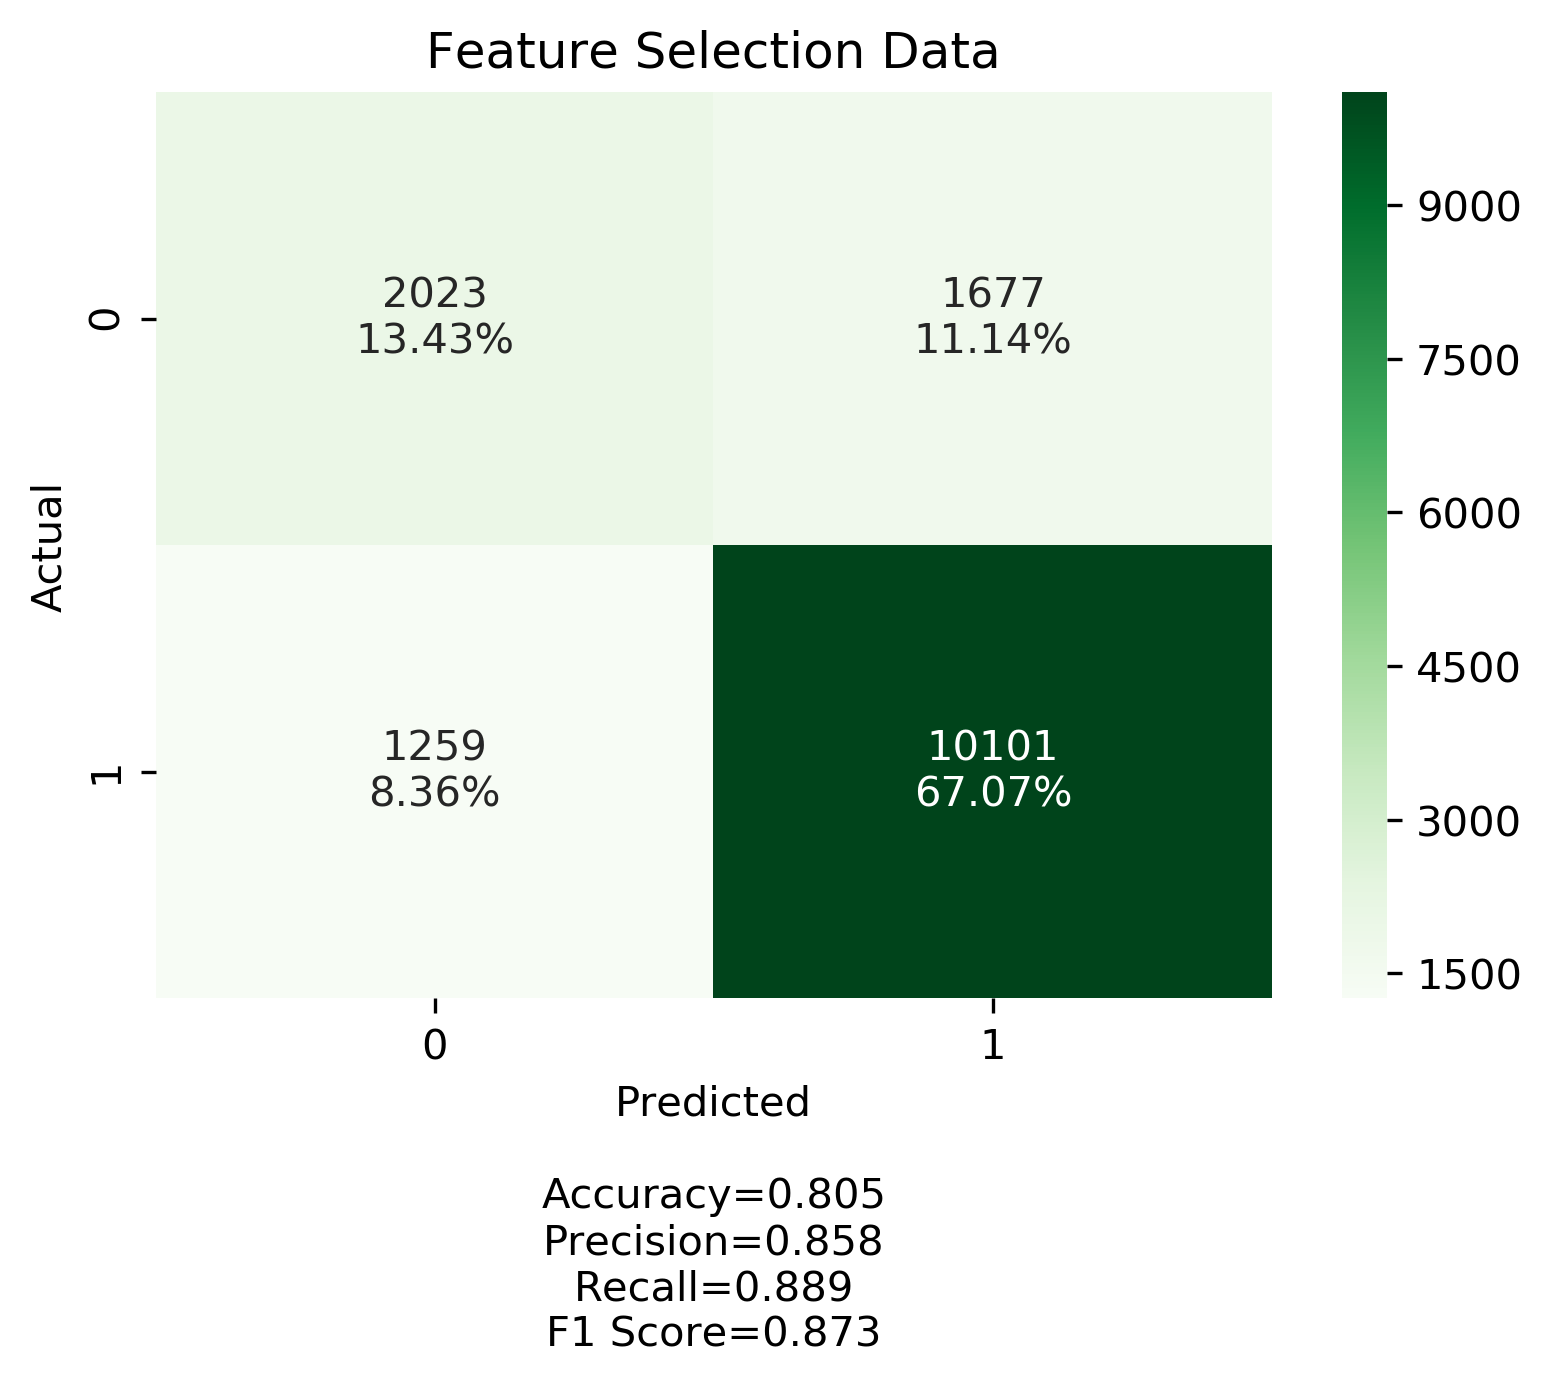
\includegraphics[width=.45\textwidth]{images/cf23.png}
			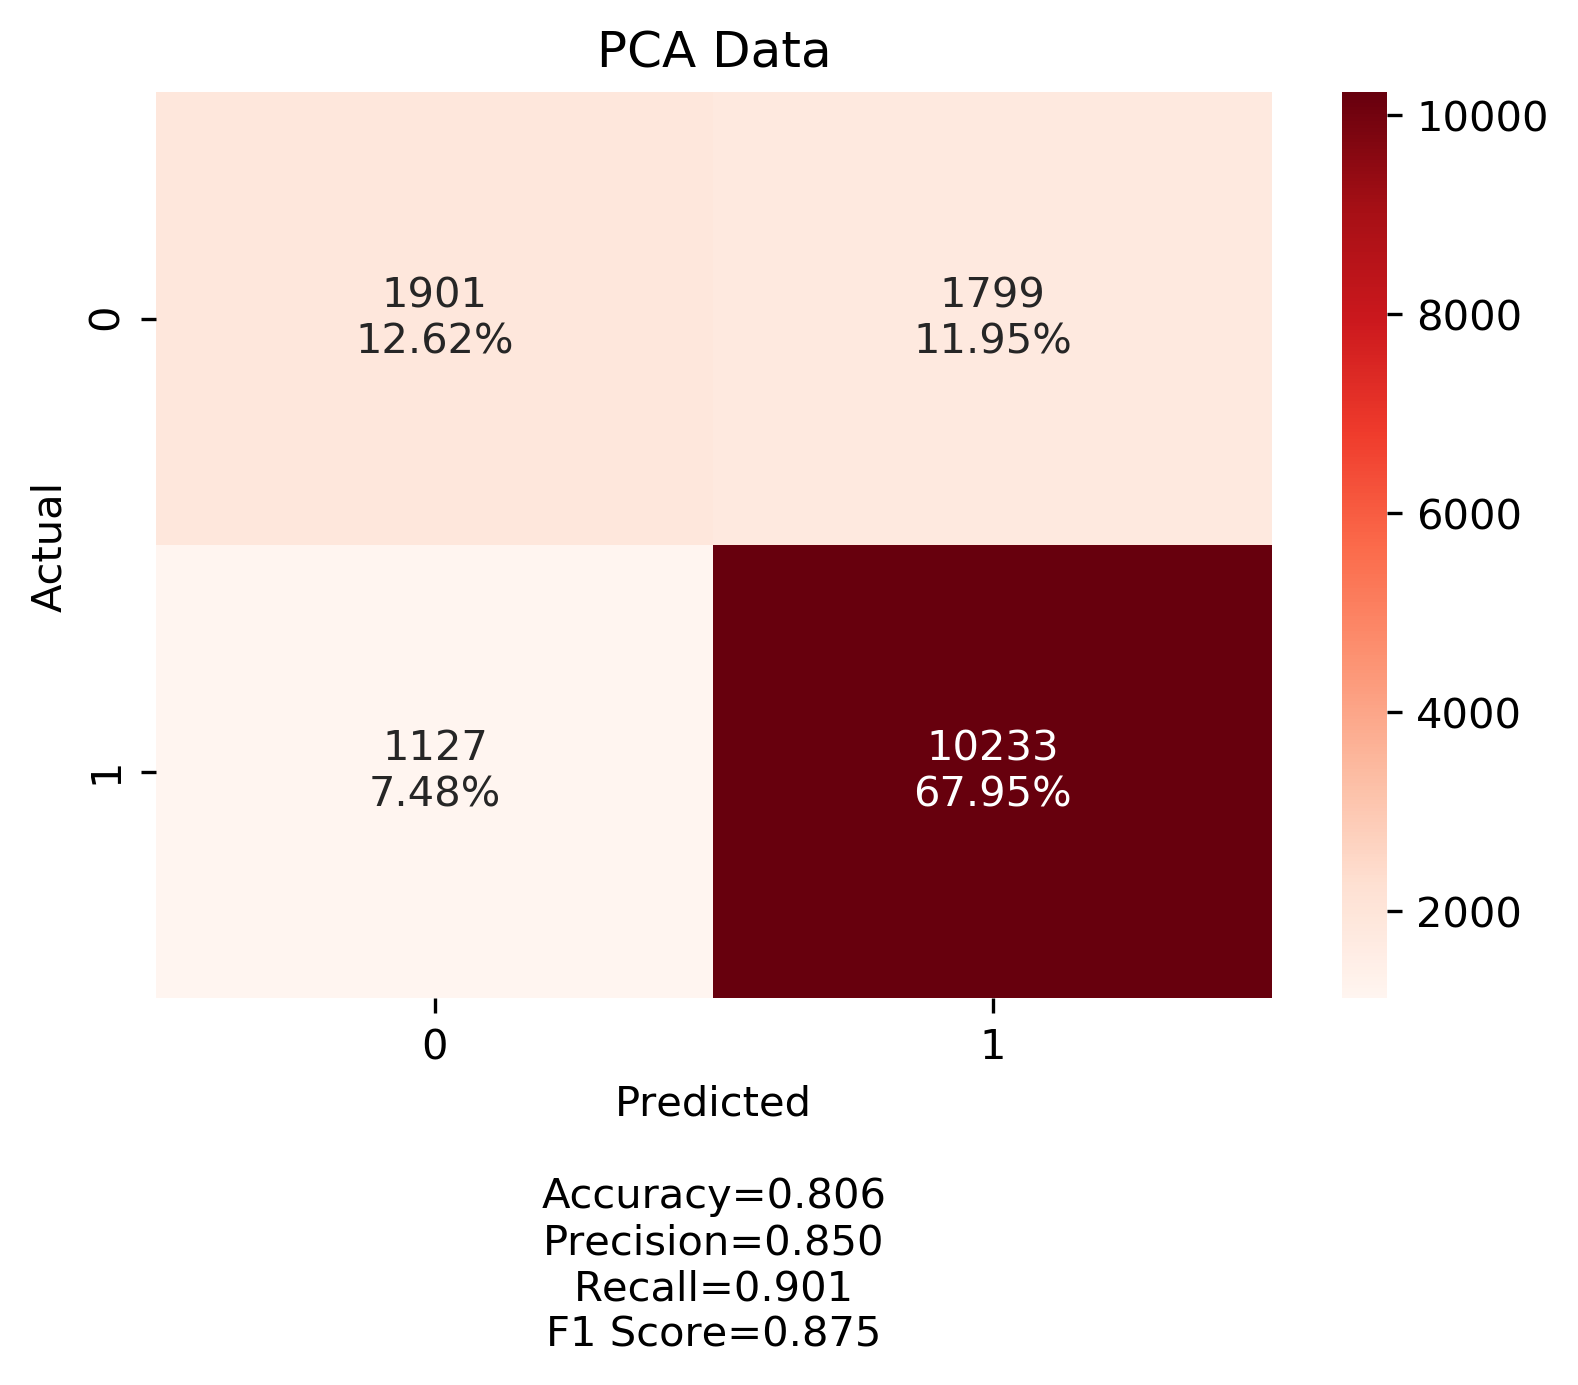
\includegraphics[width=.45\textwidth]{images/cf24.png}		
		\end{center}
	
		Things to Consider:
		\begin{itemize}
			\item Can be slow to implement as there are many different decision trees to be first made
			\item Works well for categorical data and non-normalized
			\item Pre/Post pruning may be necessary to optimize results (without over fitting)
		\end{itemize}			
		\newpage
		\subsection{K-Means}~
				
			This unsupervised algorithm is based on finding $ k $ clusters in the geometric space of the data. This is found by measuring the distance of each cluster node $ \mathbf{p} $ to every data point in the set. The minimal distance is then chosen for each data point and the $ k $-cluster points are then shifted and tested again until some convergence occurs.
			
			\begin{equation}
				min (dist_{i})	 = min || \mathbf{p_j} - \mathbf{x}_i ||_2\quad \forall j
			\end{equation}
			$ \mathbf{p_j} =$ some cluster point $ j = 1,2,...,k $\\

			We experimented with the number of clusters and determined that 2 gave us the best results. As the number of clusters increases, more assistance is needed from the training classifications to identify which cluster point corresponds to which class. Since providing this assistance would make this algorithm more \emph{supervised}, we decided we would minimize our assistance and emphasize the difference between supervised and unsupervised algorithms. Running this model on our four data sets results in the following confusion matrices:
		\begin{center}
			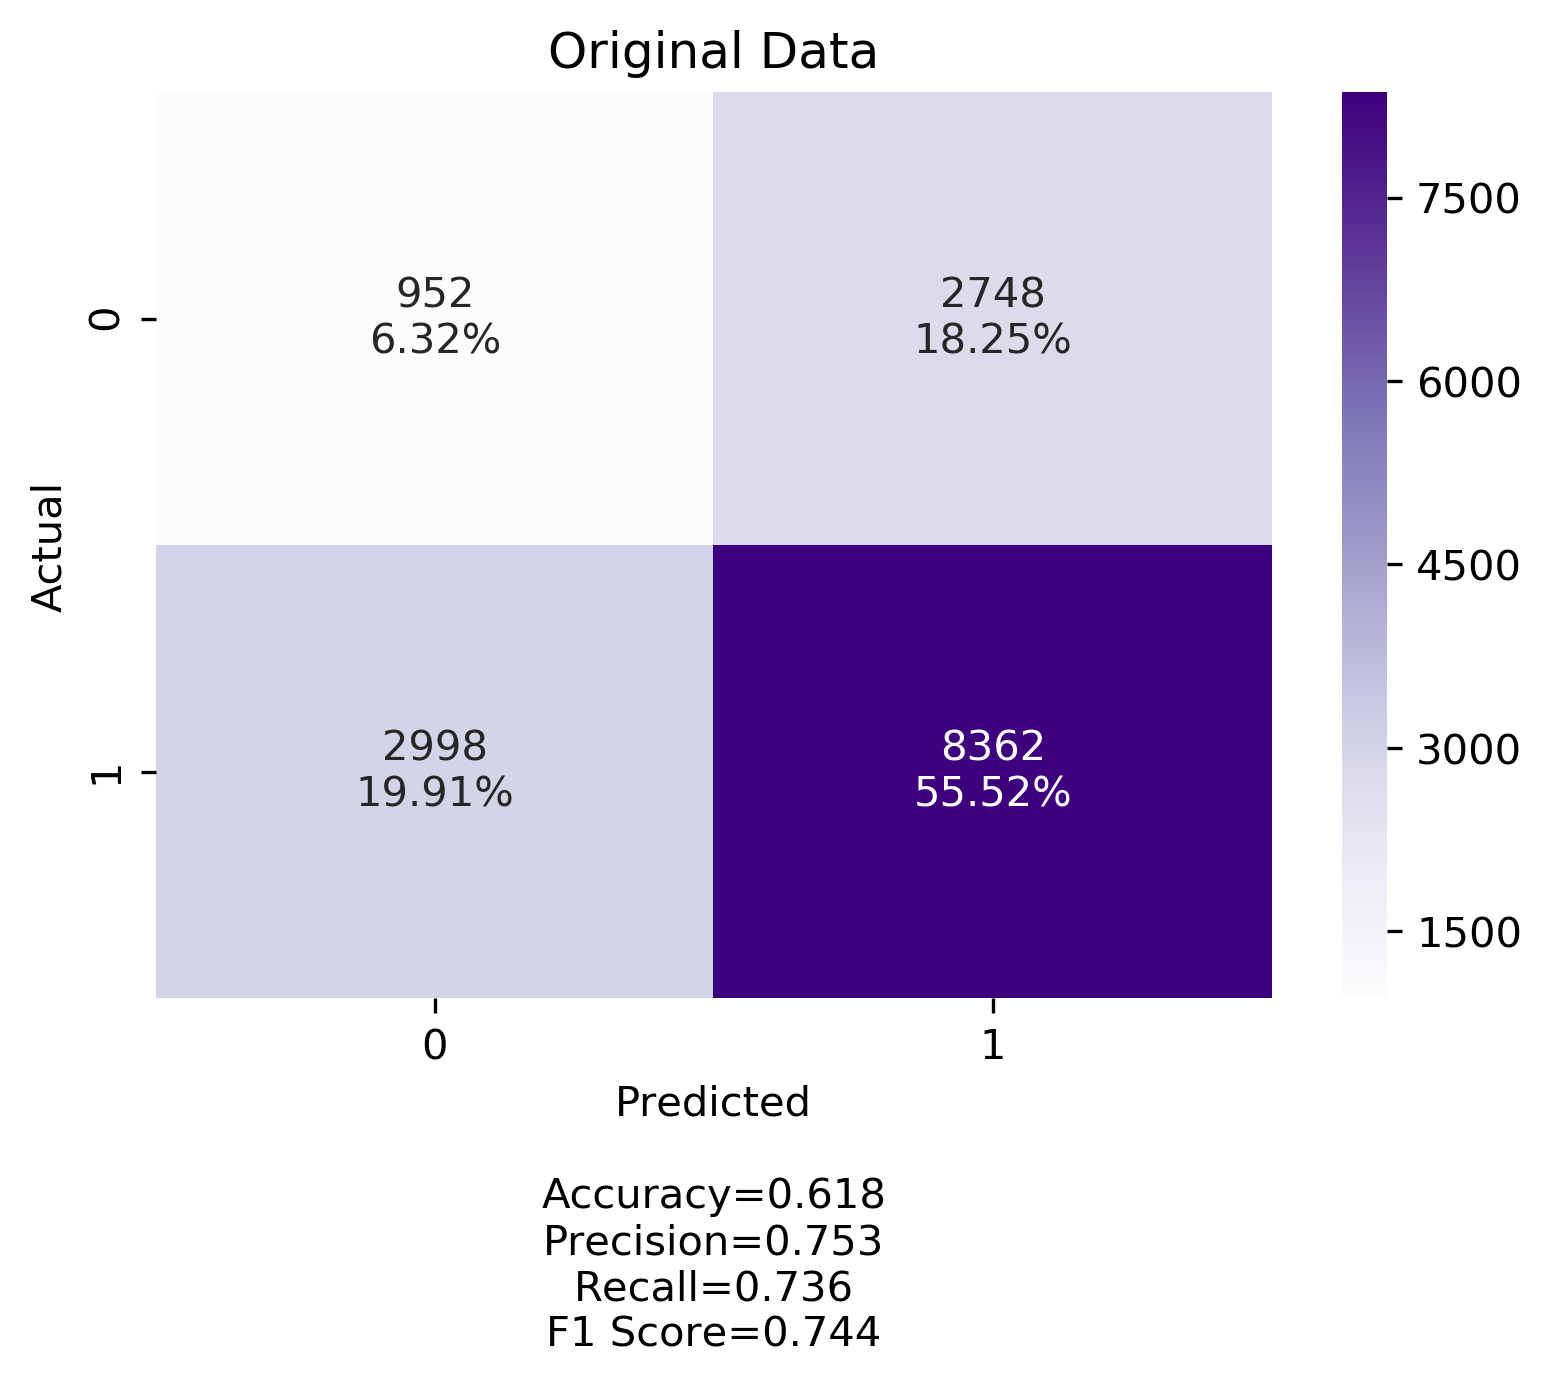
\includegraphics[width=.45\textwidth]{images/cf25.png}
			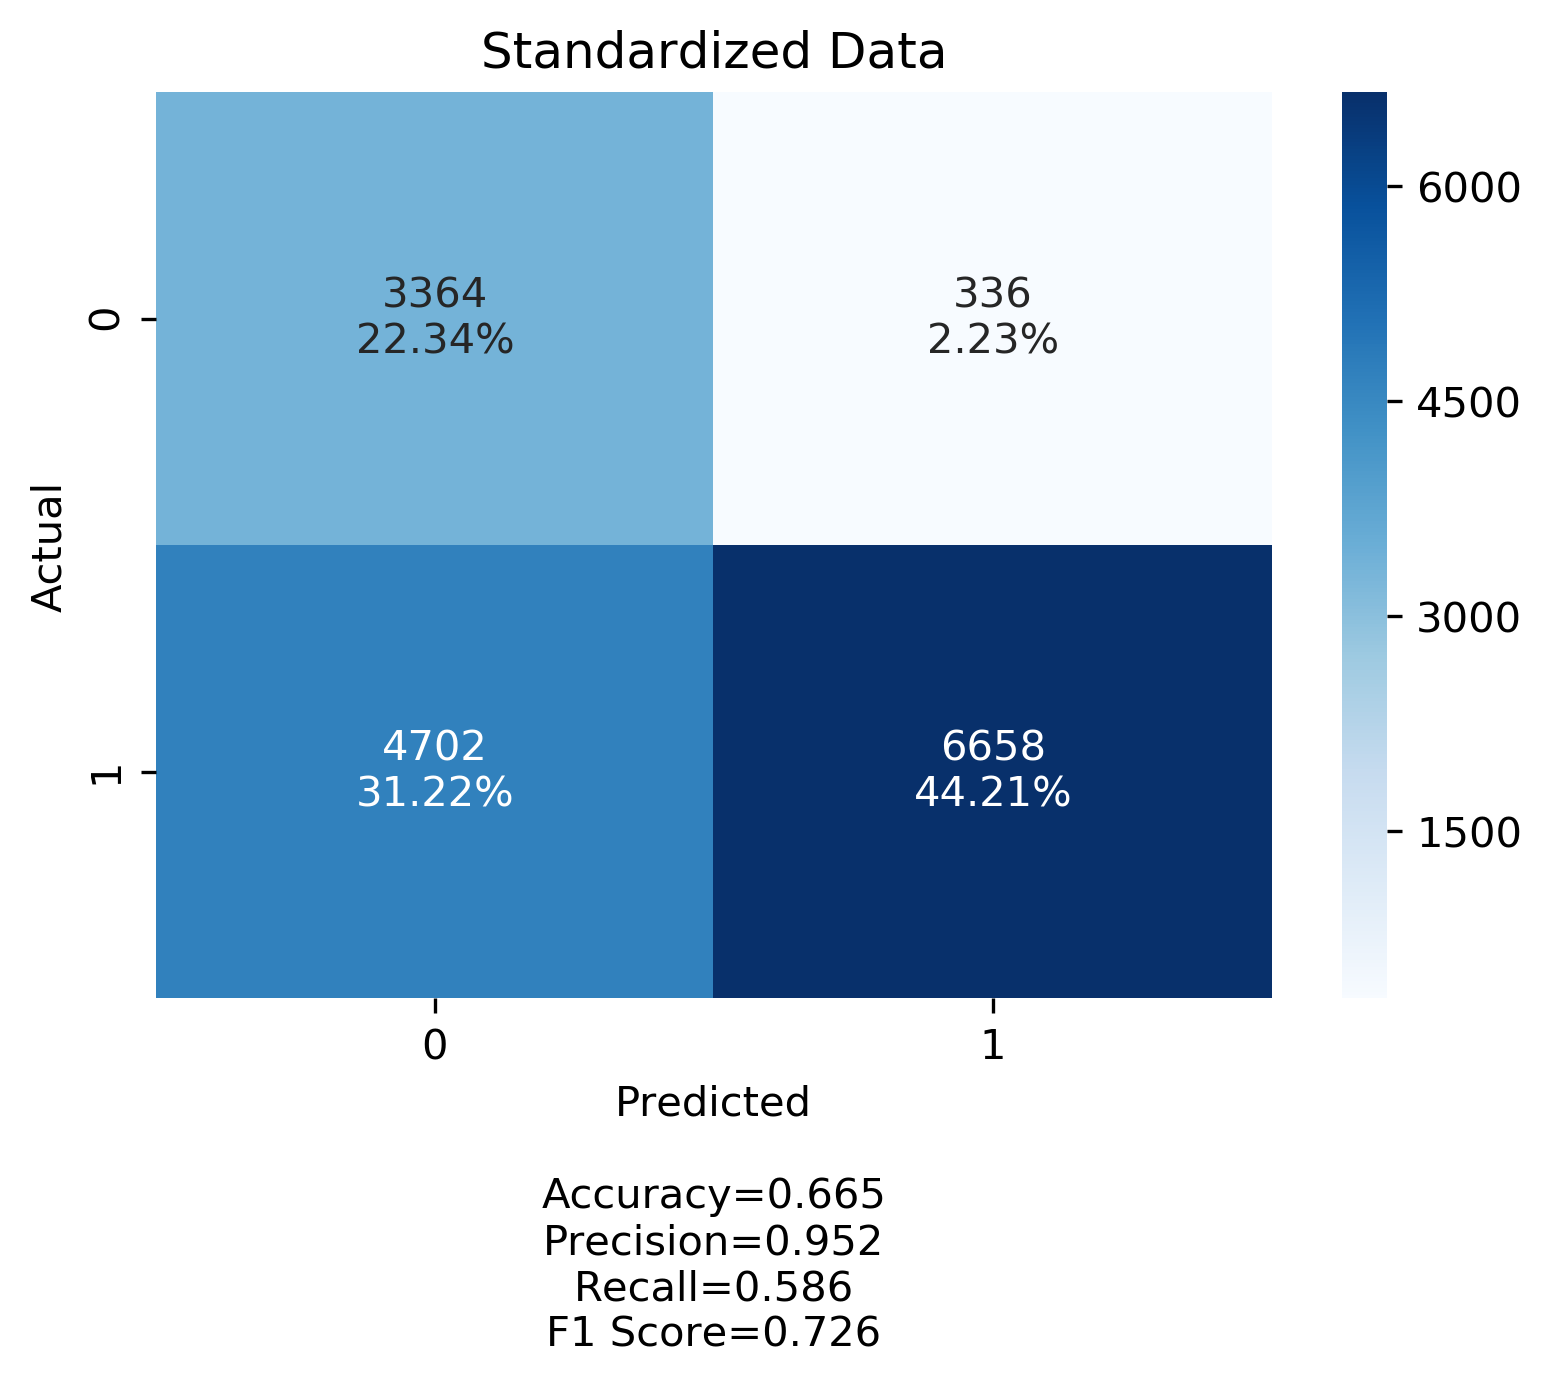
\includegraphics[width=.45\textwidth]{images/cf26.png}
			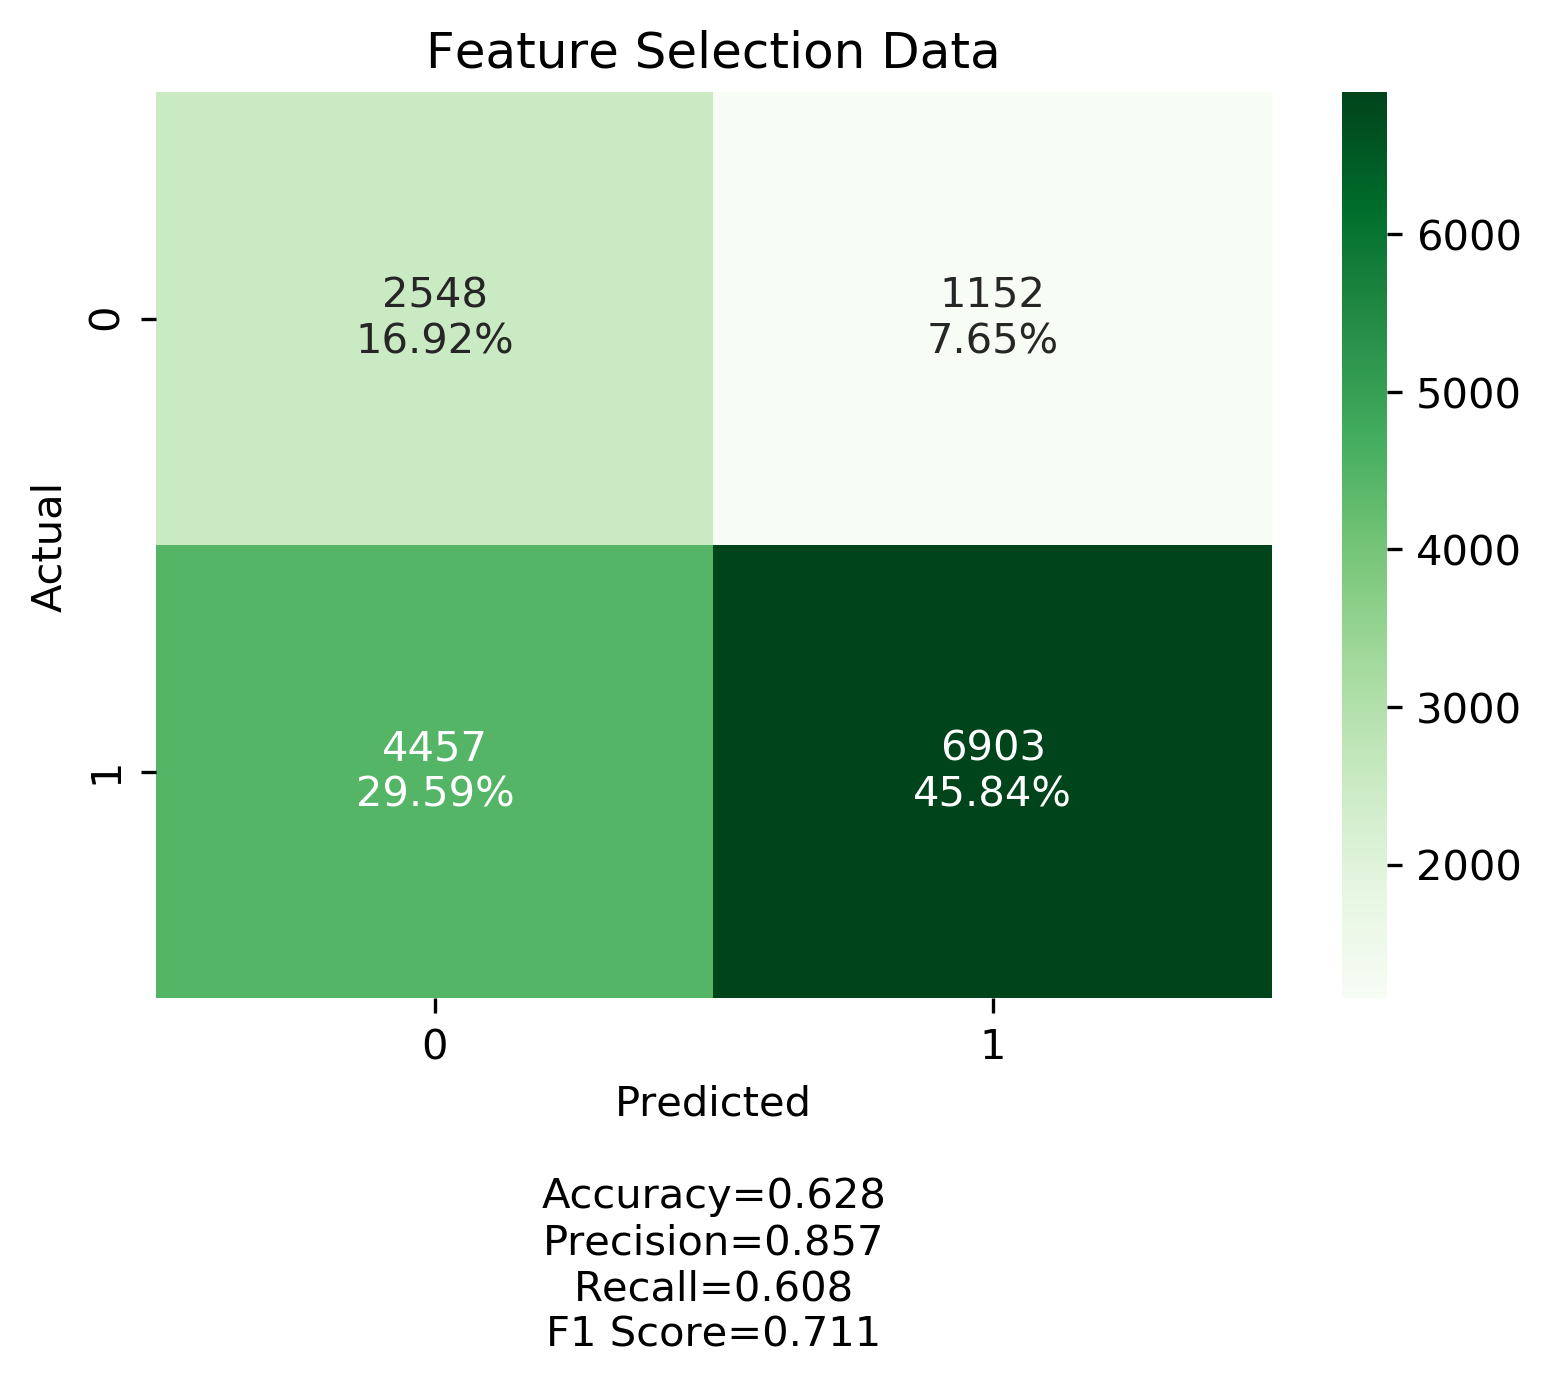
\includegraphics[width=.45\textwidth]{images/cf27.png}
			\includegraphics[width=.45\textwidth]{images/cf28.png}		
		\end{center}

		Things to Consider:
		\begin{itemize}
			\item This algorithm does not work well for data that is not easily separable (which is the case here)
			\item As we increase the dimensions each computation becomes a little harder, though the results will generally become better
		\end{itemize}		
		
		\subsection{Ensemble}~
		
		An ensemble learner simply uses the classifications determined by other algorithms to develop its own classification. This can come in the form of taking a vote between the classifications and choosing the most popular one, taking an average of the classifications, or potentially implementing more complex techniques. For our purposes the vote technique suffices as we are dealing with a binary class. Modifying the class values to be $ \text-1 $ or $ 1 $ allowed us to take a sum of the other classifications and simply choose $ \text-1 $ if our sum was negative and choose $ 1 $ if our sum was positive.\\
		
		
		Running this model on our four data sets results in the following confusion matrices:
		\begin{center}
			\includegraphics[width=.45\textwidth]{images/cf29.png}
			\includegraphics[width=.45\textwidth]{images/cf30.png}
			\includegraphics[width=.45\textwidth]{images/cf31.png}
			\includegraphics[width=.45\textwidth]{images/cf32.png}		
		\end{center}
		
		Things to Consider:
		\begin{itemize}
			\item Works most effectively with a variety of other approaches, possible weighting may be necessary 
			\item This classifier is dependent on all other classifiers and cannot be used alone
		\end{itemize}
		
	\section{Conclusion}


	\subsection{Results}
	
	\begin{tabular}{c|cccc|c}
		Model Accuracy & Original & Standardized & Feature Selection & PCA & Average\\
		\hline
		Naive Bayes & $78.9\%$&$81.1\%$ &$77.3\%$ &$80.4\%$ &$79.43\%$\\
		Logistical Regression & $79.3\%$& $83.8\%$ &$81.4\%$ &$81.3\%$&$81.45\%$\\
		Linear Regression &$81.8\%$ &$81.7\%$ &$80.7\%$ &$80.2\%$&$81.1\%$\\
		Support Vector Machine &$79.1\%$ &$84.5\%$ & $81.9\%$ &$81.3\%$&$81.7\%$\\
		Decision Tree & $80.5\%$ & $80.1\%$&$78.9\%$ &$74.8\%$&$78.58\%$\\
		Random Forest &$85.8\%$ & $85.5\%$&$80.5\%$ &$80.6\%$&$83.1\%$\\
		K-Means &$61.8\%$ & $66.5\%$&$62.8\%$ &$64.6\%$&$63.93\%$\\
		Ensemble &$82.5\%$ & $84.7\%$&$81.4\%$ &$81.3\%$&$82.475\%$\\
		\hline
		Average &$78.71\%$ & $80.99\%$&$78.11\%$ &$78.06\%$&\\
		 
	\end{tabular}
	
	\subsection{Discussion}~
	We divide our discussion into two sections: one focusing on the data transformations used and one focusing on the classifier algorithms used.
	\subsubsection{Data Transformation}~
	The obvious winner, in terms of accuracy of the different data transformation techniques is the standardization method. It was consistently near the top for every algorithm. The important thing to note here is that it took care of outliers in the data without losing any information.\\
	
	It is worth noting, however, that the advantages of feature selection and PCA, while not clear here, are still present. During our feature analysis we saw that nearly every attribute of the data set was useful for determining the class. We chose to remove half of the attributes, but it may have been better to only remove a few. With further experimentation we could determine the most ideal number and combination of features to exclude.\\
	
	PCA did fairly well considering it shrunk information from 14 columns into 5 columns. The main advantage of PCA (and feature selection) is not its increase in accuracy, but its decrease in space and increase in speed, both of which were not measured in this report.	This can be shown in the running of the notebook Project.ipynb.
	
	\subsubsection{Classifier Algorithms}~
	
	The most accurate algorithm was clearly the random forest algorithm. However, this algorithm is fairly slow compared to most others (as you can verify in the jupyter notebook). Random forest is a type of ensemble learner because it classifies based on the results of many small decision trees.\\
	Next in line was the explicit ensemble learner which is limited by the accuracy of all the other algorithms. The main advantage is that in most cases, even if a couple algorithms classified a point wrong, we expect that most algorithms classified it correctly. This is the main way ensemble learners reduce error. Although running the ensemble learner is fast, it must be preceded by other algorithms, so any speed advantage it has is null.\\
	
	According to our results, the third best algorithm, in terms of accuracy, is SVM. However, running this algorithm took the longest by far (it made random forest seem fast). Originally, we desired to run a linear SVM algorithm on the data set, but it would not converge due to the inseparability of the data set alluded to previously. We therefore needed to use a variation of SVM that ended up overfitting the data (available in the notebook).\\
	
	Given the data was not easily separable, this impacted the effectiveness of the K-Means algorithm causing it to perform rather poorly. In addition, there may be a more ideal value for the number of clusters, but as previously discussed, we decided to let the algorithm remain relatively unsupervised. Testing with 4 clusters provided even more inaccurate results.
	
	\subsection{Further Possibilities}~
	
	Overall, our models failed to predict salary with sufficient accuracy. However, to improve our models in further iterations there are several methods that could increase our accuracy and sensitivity, without simply increasing the size of the dataset.\\
	
	The first option is to use a derivation of random sub-sampling, a method which allows the model to train several times on each data point without over-fitting. The basic idea is, during each round of training, instead of iterating through the whole dataset a small number of times, to instead iterate many times over smaller subsets, determined either at complete random, or via an algorithm. This allows more overall training time without overfitting the model, allowing a smaller dataset to essentially act as a larger one and boost performance.\\
	
	Another option to increase the effective size of our dataset, and therefore performance, is called Cross-validation. In this method, a training set is left out during each training epoch as normal, but instead of having a fixed test set or culling the entire dataset, the test set progresses through the entire training set according to some scheme that ensures all data is tested on at some point. Since this method maximizes the training data at every iteration and doesn't require the total exclusion of the training set, it can often lead to better results.\\

	Overall, there are many options to optimize our training models using many facets of data science. Fully exploring these options will most certainty lead to more interesting options.
% This is a dumb AF conclusion, but someone who is not completely demolished please make it more ad-speak for the prof or whomstever grades these things.	
		% some active learning from the original data sets. and the test data, allowing the algorithm to further intensify its results.

	\newpage
	\section{References}~
% \textbf{ADD ANY REFERENCES USED HERE IN A BIBLIOGRAPHY ALSO MAKE OFFICIAL LOOKING (FORMAT WISE)}




% Notes from Alex Thomo Class\\
[1]  $\>$ Alex Thomo, SENG 474 Lecture Notes, Fall 2019, University of Victoria\\

[2]  $\>$ M. Ai, J. Yu, H. Zhang, and H. Wang, “Optimal Subsampling Algorithms For Big Data Regressions,” Statistica Sinica, Jun. 2019.\\

% Dataset: 
% \href{https://archive.ics.uci.edu/ml/datasets/Adult}{https://archive.ics.uci.edu/ml/datasets/Adult}\\
[3] $\>$ Ronny Kohavi and Barry Becker, "1994 Census Database", 1994.\\

[4]  $\>$ R Core Team (2019). R: A language and environment for statistical computing. R Foundation for Statistical Computing, Vienna, Austria. URL https://www.R-project.org/.\\

[5] $\>$ Scikit-learn: Machine Learning in Python, Pedregosa et al., JMLR 12, pp. 2825-2830, 2011.\\

[6] $\>$ McKinney, W. et al., 2010. Data structures for statistical computing in python. In Proceedings of the 9th Python in Science Conference. pp. 51–56.\\

[7] $\>$ Oliphant, T.E., 2006. A guide to NumPy, Trelgol Publishing USA.\\

[8] $\>$ Georgios Drakos, "Cross-Validation, " Towards Data Science, Aug. 2018.\\

% Python - Sklearn, Pandas, Numpy\\~\\
% \href{http://jmlr.csail.mit.edu/papers/v12/pedregosa11a.html}{Scikit-learn: Machine Learning in Python}, Pedregosa et al., JMLR 12, pp. 2825-2830, 2011.\\~\\



[9] $\>$ Wu-Sheng Lu, ECE 403 Lecture Notes Ch. 1, June 2019, University of Victoria\\

\end{document}